%!TEX root = these.tex

\chapter[Taxinomie des environnements de sélection]{Taxinomie des environnements de sélection}
\minitoc
\label{chap3}
\cleardoublepage

\section{Introduction}

	\subsection{Nature des cibles}
	Au cours du premier chapitre de ce manuscrit, nous avons identifié un certain nombre de besoins associés à des applications précises. Nous nous sommes également attachés à caractériser la nature des cibles mobiles que l'on rencontre dans ces applications, afin de permettre au lecteur d'apprécier d'une part l'ensemble des difficultés inhérentes aux tâches de sélection dans ces applications, et d'autre part la nécessité d'une assistance à la sélection.
	
	Si nous avons jusqu'ici énuméré et caractérisé ces types de cibles, avec une attention toute particulière à leur contexte applicatif, nous n'avons pas procédé à une classification systématique des cibles selon la nature de leur mouvement, définie selon des critères objectifs et des mesures quantitatives.
	
	Or, il nous apparaît que pour réellement comprendre les enjeux et défis liés à la sélection de cibles mobiles, une telle classification est nécessaire. L'objectif de ce chapitre est donc d'établir une taxinomie des cibles mobiles selon des critères objectifs et, dans la mesure du possible, permettant une quantification des valeurs auxquelles ils se rapportent.
	
	\subsection{Nature des environnements}
	Bien qu'une \og simple \fg{} taxinomie des cibles mobiles en fonction de la nature de leur mouvement ait beaucoup d'intérêt, elle ne saurait fournir suffisamment d'informations pour guider la conception de techniques de sélection sans tenir compte de l'\emph{environnement} de sélection. En effet, la cible la plus petite, la plus rapide et la plus imprévisible qui soit est triviale à sélectionner s'il s'agit du seul objet d'intérêt dans l'environnement : il n'y a qu'une sélection possible, donc la technique de sélection optimale --- ou du moins suffisante --- consiste à permettre la sélection de la cible par la simple pression d'un bouton, ou activation d'un quelconque périphérique de saisie.
	
	En effet, du point de vue de la théorie de l'information de Shannon~\cite{shannon2001mathematical}, un seul bit d'information est à transmettre de l'utilisateur au système, correspondant à la réponse à la question suivante : \og la cible doit-elle être sélectionnée ? \fg{}. Si la réponse est négative, l'utilisateur ne fait rien et le système non plus ; si elle est positive, une seule action est nécessaire de la part de l'utilisateur, et le système, qui connaît la position de la cible, n'a qu'à la sélectionner sans requérir de précision de la part de l'utilisateur.
	
	Même dans un cas où il y aurait plusieurs objets de ce type, mais en petit nombre, la sélection demeurerait relativement aisée avec une technique telle que le \emph{Bubble Cursor}, analysé au cours du deuxième chapitre. En effet, cette technique illustrée par la figure~\ref{fig:bubble} partage l'espace en plusieurs cellules, selon un diagramme de Voronoï (voire figure~\ref{fig:voronoi}). De fait, avec par exemple quatre cibles (éventuellement très petites, rapides et imprévisibles) l'espace virtuel serait partagé en quatre parties qui, la plupart du temps, serait très grandes. La loi de Fitts ne s'appliquerait pas directement, car ces zones de sélection seraient mobiles, mais l'on voit bien que la sélection ne serait pas très difficile.
	
	À l'inverse, avec des cibles aussi petites, rapides et imprévisibles, mais extrêmement nombreuses, l'on comprend aisément que l'intérêt du \emph{Bubble Cursor} serait très fortement diminué car les cellules de Voronoï de chaque cible deviendraient fort petites, et pas nécessairement significativement plus grandes que les cibles elles-mêmes.
	
	Il apparaît donc clairement que la difficulté d'une tâche de sélection ne peut être évaluée qu'en tenant compte de l'environnement dans lequel l'objet ciblé est sélectionné. De fait, les besoins et contraintes devant orienter la conception d'une technique d'assistance doivent également en tenir compte. Aussi notre taxinomie tiendra-t-elle compte de l'environnement global, et non seulement de la cible à sélectionner et de la nature de ses mouvements.
	
	\subsection{Critères subjectifs}
	Nous verrons plus loin que des critères plus subjectifs --- quoique fondés sur des observations empiriques --- peuvent être plus pertinents pour estimer la difficulté d'une tâche de sélection, et nous proposerons une taxinomie révisée en conséquence.

\section{Taxinomie des environnements de sélection}

    \subsection{Critères de discrimination}
    L'établissement de notre taxinomie passe par le choix des critères qui nous permettront de d'établir des distinctions entre les types de mouvements des cibles et les environnements de sélection. Dans les sous-sections suivantes, nous allons détailler les critères que nous avons retenus.

    \subsubsection{Autocorrélation}
    Nous considérerons ici qu'un mouvement est autocorrélé si un \emph{changement de direction} opéré à l'instant $t$ dépend du \emph{changement} (éventuellement nul) opéré à l'instant $t-1$. Si, au contraire, un changement peut avoir lieu à l'instant $t$ quel que fût la situation à l'instant précédent, nous appellerons ce mouvement \emph{markovien}~\cite{markov1960theory} en admettant qu'il s'agit d'un abus de langage, puisqu'un processus respectant la propriété de Markov est totalement indépendant de l'état du système à l'instant précédent ; or, ici, le vecteur direction d'un objet à l'instant $t$ peut dépendre de son orientation à l'instant $t-t$ même si le changement d'orientation n'en dépend pas.
    
    En effet, si ledit changement se fait selon un angle borné (entre -45\textdegree{} et +45\textdegree{}, par exemple) alors l'orientation du vecteur direction à l'instant $t$ dépendra de son orientation à $t-1$. Tant que le changement de direction à l'instant $t$, lui, est bien indépendant du changement à l'instant $t-1$ nous admettrons cet abus de langage et parlerons de mouvement markovien ; sinon, le mouvement sera dit autocorrélé. Par commodité, un objet dont les mouvements sont autocorrélés sera dit autocorrélé, et un objet dont les mouvements sont markoviens sera dit markovien.
    
    Concrètement, les objets macroscopiques dont les mouvements sont soumis aux lois de la physique newtonienne~\cite{newton1833philosophiae} ont des mouvements autocorrélés --- ce sera donc le cas de véhicules de tous types, des êtres vivants (athlètes compris) des projectiles, missiles, etc. Les objets nanoscopiques dont les mouvements sont soumis aux lois de la mécanique quantique ont des mouvements markoviens --- ce sera notamment le cas des particules dans les simulations moléculaires. Les objets pouvant être sélectionnés dans les jeux vidéo seront autocorrélés ou markoviens, selon les règles choisies par les développeurs.

    \paragraph{Uniformité.}
    Le mouvement autocorrélé le plus simple est le mouvement uniforme, c'est-à-dire celui pour lequel le vecteur direction ne change jamais. Les objets de mouvement uniforme se déplacent donc en ligne droite. Inversement, un mouvement n'est pas uniforme si, à un instant quelconque, le vecteur direction de l'objet concerné change.

    \paragraph{Périodicité.}
    Un mouvement sera dit périodique si les changements de directions sont tels que l'objet effectuera une trajectoire fermée qu'il répétera à intervalles réguliers. Plus formellement, un mouvement est périodique s'il admet une période $T$ telle que :
    $\forall t,~Position_{t}~=~Position_{t+T}$ où $Position_{t}$ désigne la position de l'objet à l'instant $t$.
    
    \subparagraph{Pseudo-périodicité.}
    Nous appellerons pseudo-périodique un mouvement caractérisé par une trajectoire fermée et répétée à intervalles \emph{irréguliers}. Un tel mouvement ne satisfait pas la condition formalisée ci-dessus, mais admet un ensemble de positions limitées à une trajectoire donnée, et revisitées continuellement dans le même ordre --- simplement, à des vitesses pouvant varier.

    \subparagraph{Circularité.}
    Le mouvement circulaire est un cas particulier du mouvement périodique. Comme son nom l'indique assez clairement, il s'agit d'un mouvement suivant une trajectoire circulaire. Il peut également être pseudo-périodique.
    
    \subsubsection{Vitesse}
    La vitesse des cibles est un critère essentiel de notre taxinomie, car cette valeur a une très forte influence sur la difficulté de sélection, comment le montrent notamment les résultats empiriques obtenus par Ortega~\cite{ortega2013hook} et présentés sur les figures~\ref{fig:hookRes2d} et~\ref{fig:hookRes3d}, ainsi que les travaux de Jagacinksi \emph{et al.}~\cite{jagacinski1980test} (résumés par l'équation~\ref{eq:jagacinski}) et ceux d'Al Harji \emph{et al.}~\cite{hajri2011moving} (résumés par les équations~\ref{eq:hajriC2} et~\ref{eq:hajriVW}). Comme on l'imagine aisément, plus une cible est rapide, plus elle est difficile à sélectionner. Nos propres mesures, sur lesquelles nous reviendrons en détail plus loin, le confirment.
    
    Il est important de noter que la vitesse \emph{réelle} de la cible n'est pas très importante, seule sa vitesse \emph{apparente} compte. Par exemple, la Terre effectue sa rotatio autour du Soleil à près de 30~km/s, soit 108~000~km/h. Cette vitesse réelle a pourtant peu de chances d'être un problème dans une application réelle car une telle application présenterait probablement la Terre à une échelle permettant d'observer toute son orbite (ou une grande partie de celle-ci). Or, la Terre mettant environ 365 jours à compléter son orbite, sa vitesse apparente à l'écran serait très faible, donc parfaitement gérable dans une tâche de sélection.
    
    À l'inverse, une balle de tennis est comparativement lente ($\approx$~200~km/h), mais étant observée à l'échelle d'un court de tennis (environ 24~m) sa vitesse apparente est considérable. De même, un objet dans un jeu vidéo peut se déplacer très lentement, à quelques cm/s seulement ; mais si ce mouvement est observé à l'échelle 1, alors l'objet traversera un écran standard en seulement quelques secondes, voire moins.
    
    Or, notre taxinomie vise à classifier les cibles et leurs environnements selon les difficultés de sélection qu'ils présentent et non selon leurs caractéristiques absolues ; de fait, nous nous intéresserons aux vitesses apparentes des objets examinés.
    
    Ce choix (au demeurant inévitable) est lourd de conséquence car la vitesse apparente d'un objet d'une vitesse réelle donnée dépend évidemment des conditions dans lesquelles il est affiché, en particulier de l'échelle relative à la taille du dispositif d'affichage, et de ladite taille. Elle dépend également, pour tout ce qui n'est pas joué à vitesse réelle, de la vitesse choisie pour l'animation ou la simulation (avec dans ce dernier cas une contrainte supplémentaire imposée par les performances du système). Par exemple, une vidéo peut être jouée en accéléré.
    
	\paragraph{Variabilité}
	Il serait partique de pouvoir résumer la vitesse à une variable scalaire, mais ce n'est malheureusement pas toujours possible. En effet, dans les applications identifiées le long du chapitre~\ref{chap1}, la vitesse des objets est généralement variable. L'on ne saurait donc la résumer par un simple nombre. Dans l'idéal, il serait bon de connaître toutes les vitesses atteintes par les objets de la scène, avec leurs fréquences d'occurrence ; cela nous permettrait d'en dresser un histogramme. Connaissant toutes ces valeurs, l'on pourrait les représenter de façon plus concise par une moyenne et un écart-type ; il serait sans doute opportun d'ajouter à cette représentation la vitesse maximale possible, afin de pouvoir caractériser le cas (potentiellement) le plus difficile.
	
	Pour certaines applications, il sera difficile voire impossible d'avoir des informations aussi précises. Dans ce cas, nous devrons nous contenter d'une estimation aussi précise que possible des valeurs sus-citées, par exemple d'une vitesse \og typique \fg{} et d'une vitesse maximale. Ce sera généralement suffisant pour caractériser des cibles.
	
	\subparagraph{Accélération}
	Au-delà des valeurs moyennes/typiques ou maximales de la vitesse, il peut être judicieux d'examiner dans quelle mesure la vitesse peut varier en un court laps de temps, c'est-à-dire de détailler la façon dont les objets sont susceptibles d'accélérer. En effet, un objet se déplaçant relatiement lentement peut paraître aisé à sélectionner, mais s'avérer fort difficile s'il accélère brutalement, surtout si cette accélération a lieu précisément au moment où l'utilisateur effectue son mouvement de sélection.
	
	Là encore, l'idéal serait d'avoir un histogramme, ainsi qu'une moyenne, un écart-type et une valeur maximale. L'on devra plus souvent se contenter d'une valeur typique et d'une valeur maximale estimées. Ce sera généralement suffisant pour répondre à la question primordiale concernant l'accélération : \og la cible est-elle susceptible d'accélérer brusquement ? \fg{}. Sans nous répandre en détails ici, précisons simplement que les objets accélèrent généralement d'autant plus facilement qu'ils sont légers, et que les atomes peuvent le faire brusquement, y compris dans les simulations de dynamique moléculaire.
   
    \subsubsection{Fréquence des changements de direction}
    Pour les objets macroscopiques réels, la direction est généralement soit constante, soit en changement continu. Par exemple, une automobile peut rouler droit devant elle pendant un certain temps, puis, pendant une durée généralement plus courte, suivre une trajectoire courbe caractérisée par une rotation continue de son vecteur direction. Dans ce cas, il est difficile de parler de \emph{fréquence} des changements de direction, comme s'ils étaient des événements ponctuels et discrets, à moins de considérer la cette fréquence comme étant soit nulle, soit infinie.
    
    Dans certains cas, cependant, il peut être pertinent de considérer un changement de direction relativement court et rapide comme un événément instantané se produisant à un instant bien défini. Pour reprendre l'exemple de l'automobile, il est clair que cette approximation posera généralement des problèmes pour les trajets à grande vitesse, par exemple sur les autoroutes --- les courbes y sont très douces et, de fait, les changements de direction sont lents et continus. À plus basse vitesse, cependant, et notamment pendant la circulation urbaine, il est possible d'effectuer un virage à 90\textdegree{} sur un temps beaucoup plus court. Dans ces conditions, assimiler ce virage à une rotation instantanée du vecteur direction est plus raisonnable.
    
    Les objets nanoscopiques, du moins tels qu'ils sont généralement simulés, tendant à changer de direction de manière abrupte, et la notion de fréquence de changement de direction a généralement du sens. Précisions tout de même que cette fréquence ne saurait être mesurée en temps véritable mais dans le temps de l'animation : en clair, si un atome peut changer de direction de très nombreuses fois par nanoseconde (d'où une fréquence extrêmement élevée) ce qui nous intéresse ici est la fréquence des changements de direction dans l'animation présentée à un utilisateur, car nous ne nous préoccupons que de ce qu'un utilisateur perçoit et de la mesure dans laquelle cela influe sur ses performances de sélection.
    
    Il en résulte que dans les simulations moléculaires, par exemple, cette fréquence dépend de la vitesse à laquelle on décide de jouer une animation, ou d'afficher une simulation, comme pour la vitesse des cibles.
    
    Les objets virtuels tels que ceux rencontrés dans les jeux vidéos ne sont soumis à aucune contrainte physique, et leurs directions peuvent changer de manière instantanée ou continue, selon les choix des développeurs ; dans certains cas, cette notion de fréquence aura donc du sens, et dans d'autres non.
    


    \subsubsection{Densité de l'environnement}
    Une caractérisation précise d'un environnement de sélection doit inclure une estimation de sa densité. Celle-ci peut se calculer en nombre d'objets pouvant être sélectionnés par unité de surface (pour un espace en 2D, ou un plan sur lequel un espace 3D serait projeté) ou par unité de volume. L'espace des densités est continus mais, pour les besoins de la taxinomie, on peut le discrétiser en un nombre fini de niveaux, définis par des intervalles de densité mutuellement disjoints.
    
    \paragraph{Occultation.}
    Le niveau d'occultation visuelle d'un environnement est également crucial, et notre taxinomie ne saurait l'ignorer. S'il dépend fortement de la densité de l'environnement, on ne peut établir de lien d'équivalence entre celle-ci et celui-là. En effet, pour une densité donnée, le niveau d'occultation peut être très élevé si les cibles sont très grosses et opaques ; si, en revanche, elles sont relativement petites, voire semi-transparentes, l'occultation peut être assez faible. Rappelons par exemple au lecteur que la même molécule est représentée sur la figure~\ref{fig:4awn_VdW} et sur la figure~\ref{fig:4awn_points}, mais que le niveau d'occultation est bien plus élevé dans le premier cas que dans le second.
	
    En outre, la \og taille \fg{} des cibles ne peut pas forcément s'exprimer de façon adéquate avec une valeur scalaire. En effet, si la taille d'une cible sphérique est correctement exprimée par son seul rayon, il en va autrement d'un objet d'une forme quelconque, et \emph{a fortiori} complexe.
    
    Pour ces raisons et d'autres, l'estimation du niveau d'occultation est difficile, et mériterait peut-être à elle seule de faire l'objet d'une thèse de doctorat. Peut-être serait-il opportun de la quantifier par une estimation de la probabilité qu'un objet quelconque soit totalement occulté, ou suffisamment occulté pour qu'un utilisateur manque de le remarquer avec une certaine probabilité donnée.
    
    C'est à regret que nous sommes contraints d'écarter cette proposition pour le moment et de nous contenter d'une estimation subjective de l'occultation, que nous exprimerons par un ensemble fini de niveaux. Quoi qu'il en soit, attendu qu'il est généralement nécessaire de voir ou d'avoir vu un objet pour le sélectionner, il s'agit d'un critère extrêmement important.

    \subsection{Taxinomie obtenue}
    Résultats ; appli OpenCV ?

\section{Modèle de génération de mouvement}
    \subsection{Motivations et principe}
    \subsubsection{Générer du mouvement pour mener des évaluations}
    Afin d'étudier rigoureusement la sélection de cibles mobiles en fonction de la nature du mouvement, il est nécessaire de pouvoir générer différents types de mouvements avec le plus petit nombre de paramètres possible. Dans l'idéal, le modèle choisi pour la génération de mouvement devrait être capable d'en générer une très grande variété. Les objectifs de variétés et de petitesse du nombre de paramètres étant contradictoires, un compromis doit être atteint.
    
    Sans doute de nombreux modèles pourraient-ils être conçus, et sans doute pourraient-ils correspondre à des compromis ayant divers avantages et inconvénients. Dans le but d'obtenir un modèle relativement simple (donc utilisable dans des évaluations d'une durée raisonnable pour les sujets) nous avons choisi de nous limiter aux mouvements markoviens ; ce choix fut également motivé par le fait que ces mouvements sont intrinsèquement moins prévisibles et, par conséquent, plus difficiles à anticiper --- ils rendent de fait la sélection plus difficile.
    
    \subsubsection{Trois paramètres pour le mouvement synthétique}
    Nous avons opté pour un modèle limité à trois paramètres pour définir le mouvement d'un objet de vecteur direction $\vec{dir}$ :
    \begin{enumerate}
    	\item La vitesse $V$ à laquelle l'objet se déplace ;
    	\item La fréquence $F$ des changements de $\vec{dir}$ ;
    	\item L'angle maximal $A$ de ces changements de direction : à chaque période $T = \frac{1}{F}$, $\vec{dir}$ subit une rotation d'un angle $\alpha$ échantillonné uniformément dans l'intervalle $[-A, +A]$.
    \end{enumerate}
    
    \subsection{Trajectoires obtenues}
    Des exemples de trajectoires obtenues avec ce modèles sont fournis dans la figure~\ref{fig:motion1530} avec $A=15$ et $A=30$, dans la figure~\ref{fig:motion4560} avec $A=45$ et $A=60$, dans la figure~\ref{fig:motion7590} avec $A=75$ et $A=90$, dans la figure~\ref{fig:motion105120} avec $A=105$ et $A=120$, dans la figure~\ref{fig:motion135150} avec $A=135$ et $A=150$, et dans la figure~\ref{fig:motion165180} avec $A=165$ et $A=180$. Dans tous les cas, $S=2,19$, $F$ prend les valeurs 1, 4, 8, 16, 32 et 60, et le mouvement généré dure 20 secondes.
    
    Naturellement, si la vitesse était plus élevée, les trajectoires seraient plus \og dilatées \fg{}, tandis que si elle était plus faible, elles seraient plus \og comprimées \fg{}. De plus, si $A=0$ ou $F=0$, alors il n'y a aucun changement de direction, et le mouvement est uniforme (rectiligne). Si nous avons échantillonné tous l'espace des valeurs de $A$ possibles --- de 0 à 180\textdegree{} --- nous nous sommes limités à 60~Hz pour la fréquence, d'une part parce qu'il devient difficile de percevoir une différence marquée dès qu'elle atteint une trentaine de hertz, et d'autre part parce que la plupart des dispositifs d'affichage du commerce sont limités à 60~Hz.    
    
   	\newcommand{\subImgWmo}{0.32\textwidth}
	\begin{figure}[htb]
		\begin{subfigure}[t]{\subImgWmo}
			\centering
			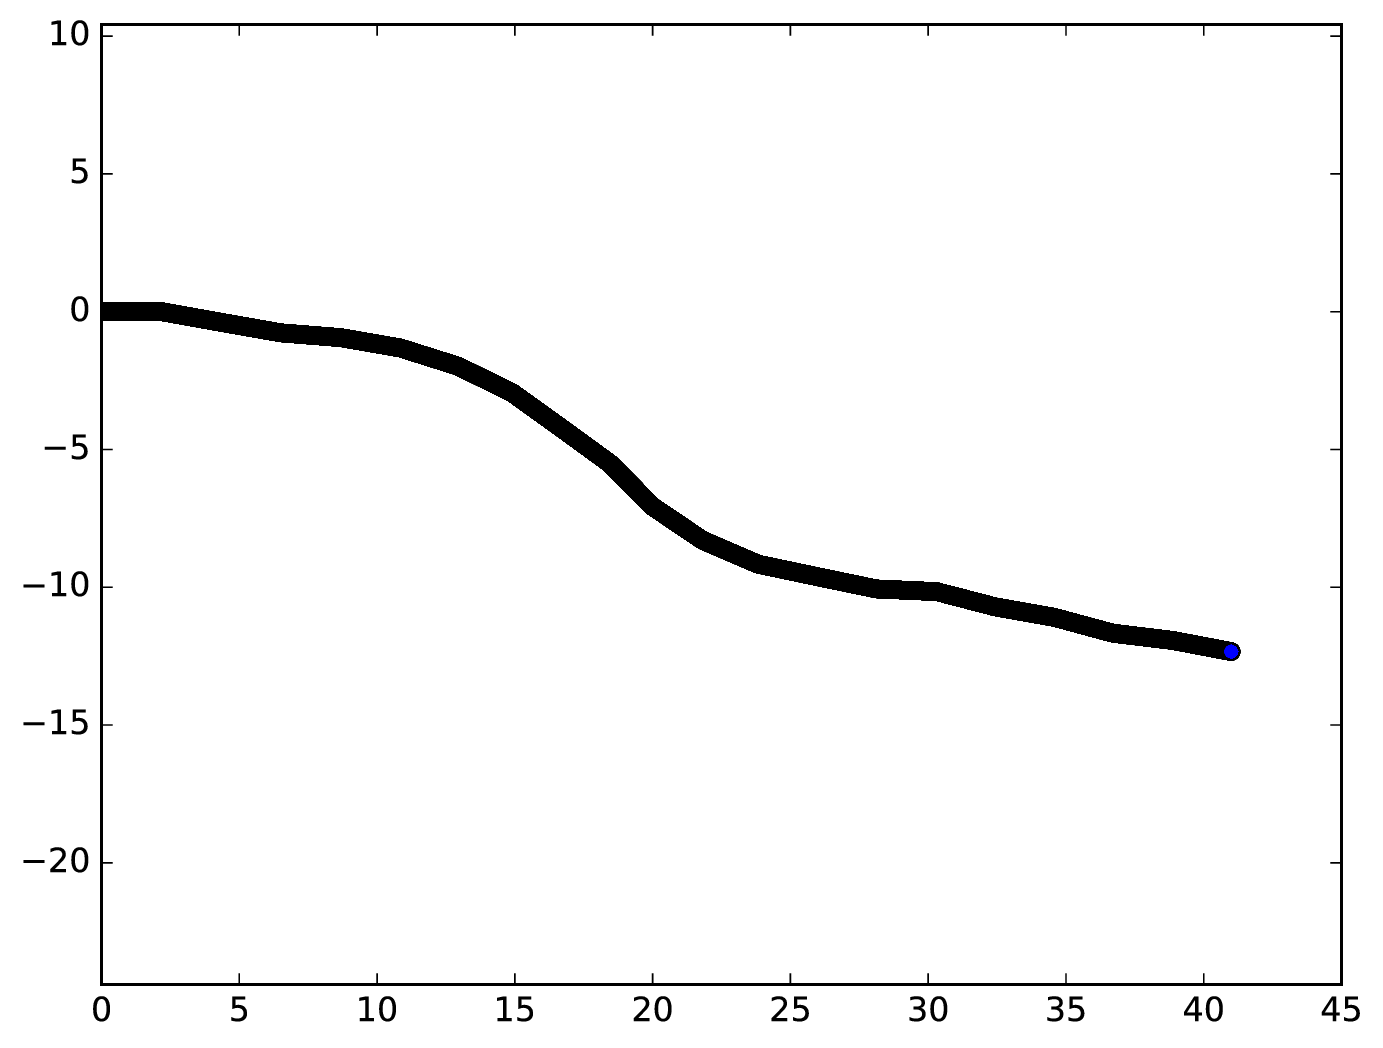
\includegraphics[width=\textwidth]{figures/ch3/synTraj_219_15_1}
			\caption[$A = 15$, $F=1$]{$A = 15$, $F=1$}
			\label{fig:synTraj_219_15_1	}
		\end{subfigure}
		~
		\begin{subfigure}[t]{\subImgWmo}
			\centering
			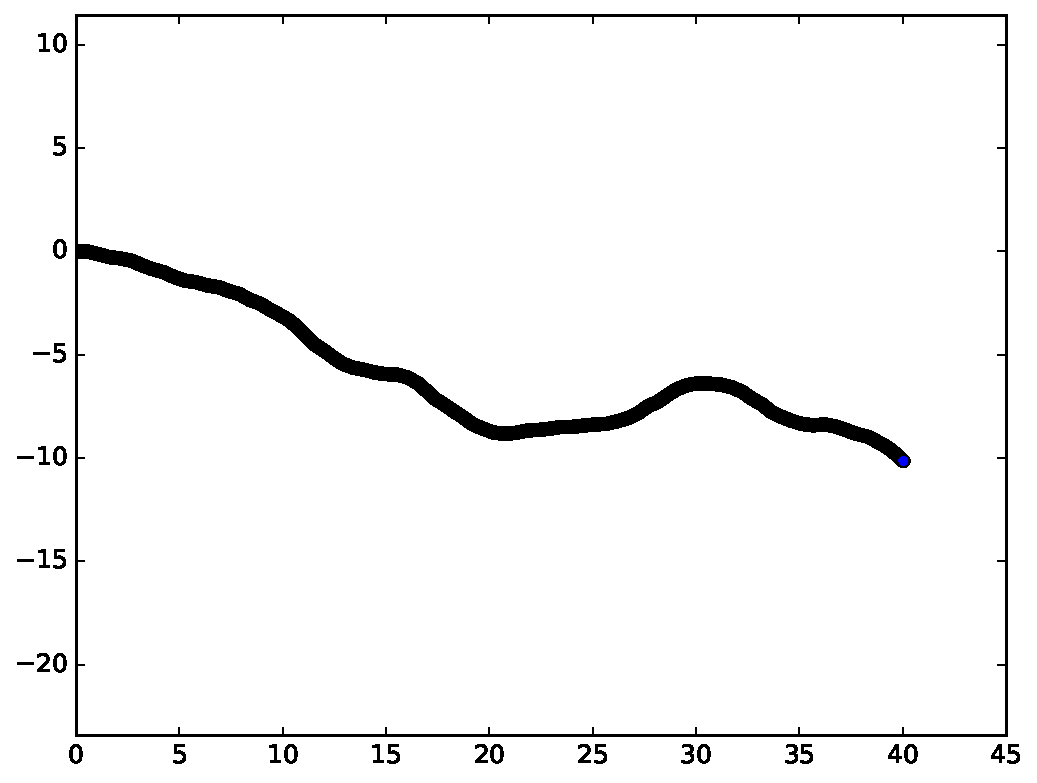
\includegraphics[width=\textwidth]{figures/ch3/synTraj_219_15_4}
			\caption[$A = 15$, $F=4$]{$A = 15$, $F=4$}
			\label{fig:synTraj_219_15_4}
		\end{subfigure}
		~
		\begin{subfigure}[t]{\subImgWmo}
			\centering
			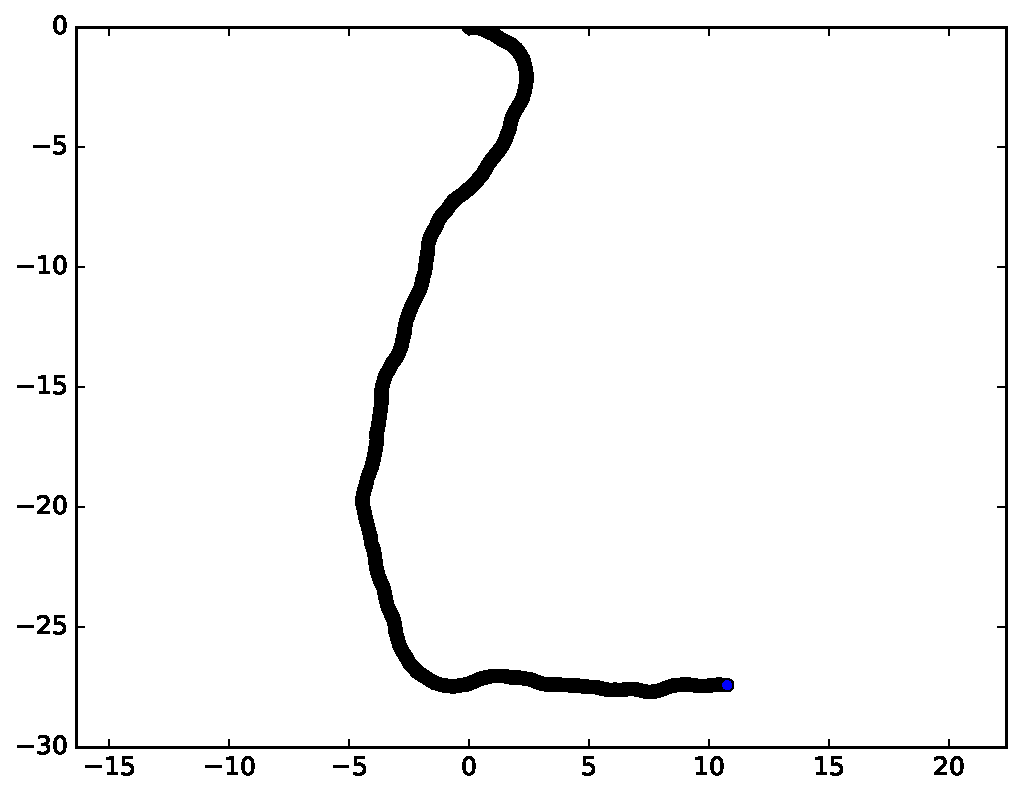
\includegraphics[width=\textwidth]{figures/ch3/synTraj_219_15_8}
			\caption[$A = 15$, $F=8$]{$A = 15$, $F=8$}
			\label{fig:synTraj_219_15_8}
		\end{subfigure}
		~
		\begin{subfigure}[t]{\subImgWmo}
			\centering
			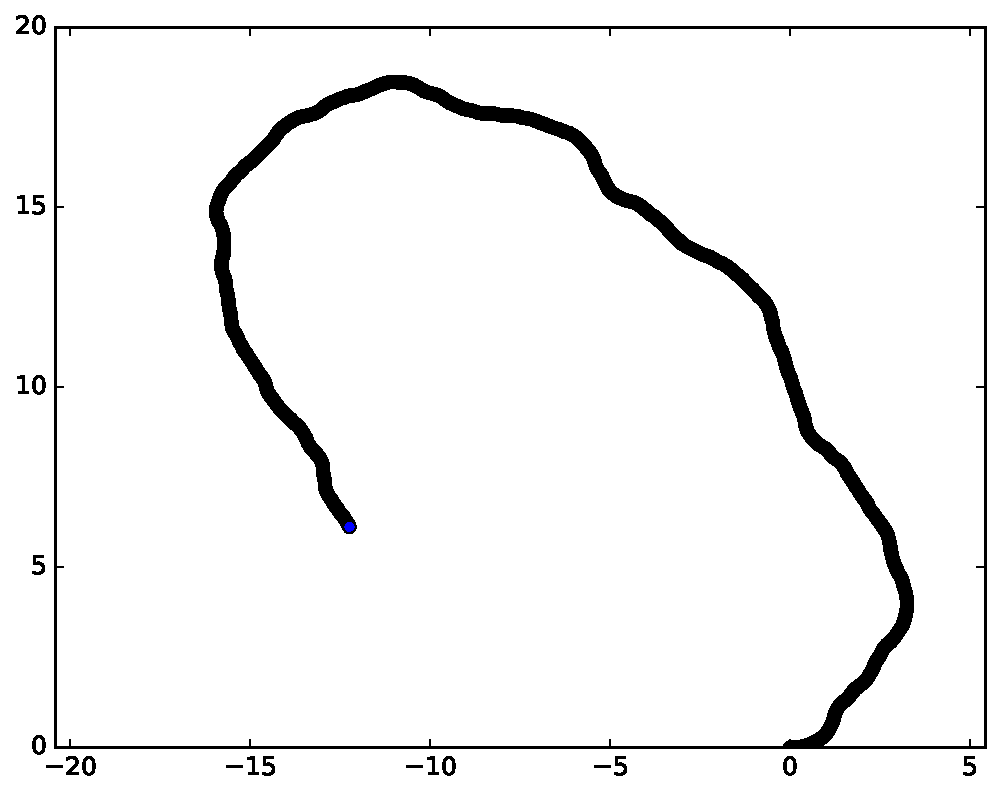
\includegraphics[width=\textwidth]{figures/ch3/synTraj_219_15_16}
			\caption[$A = 15$, $F=16$]{$A = 15$, $F=16$}
			\label{fig:synTraj_219_15_16}
		\end{subfigure}
		~
		\begin{subfigure}[t]{\subImgWmo}
			\centering
			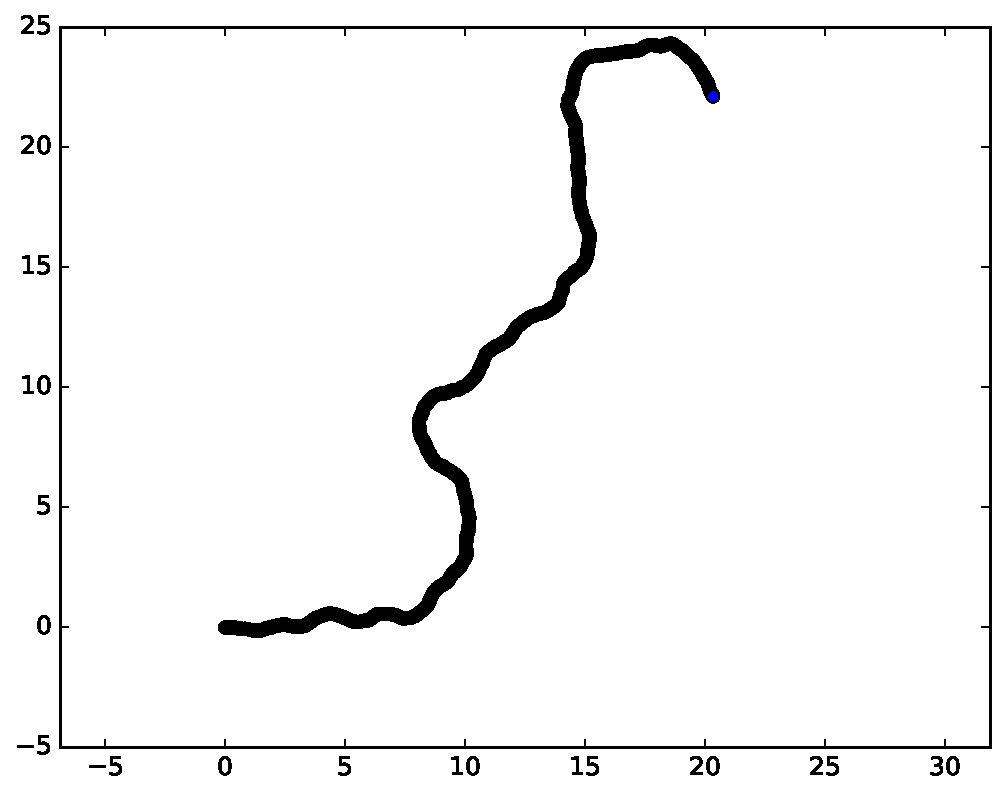
\includegraphics[width=\textwidth]{figures/ch3/synTraj_219_15_32}
			\caption[$A = 15$, $F=32$]{$A = 15$, $F=32$}
			\label{fig:synTraj_219_15_32}
		\end{subfigure}
		~
		\begin{subfigure}[t]{\subImgWmo}
			\centering
			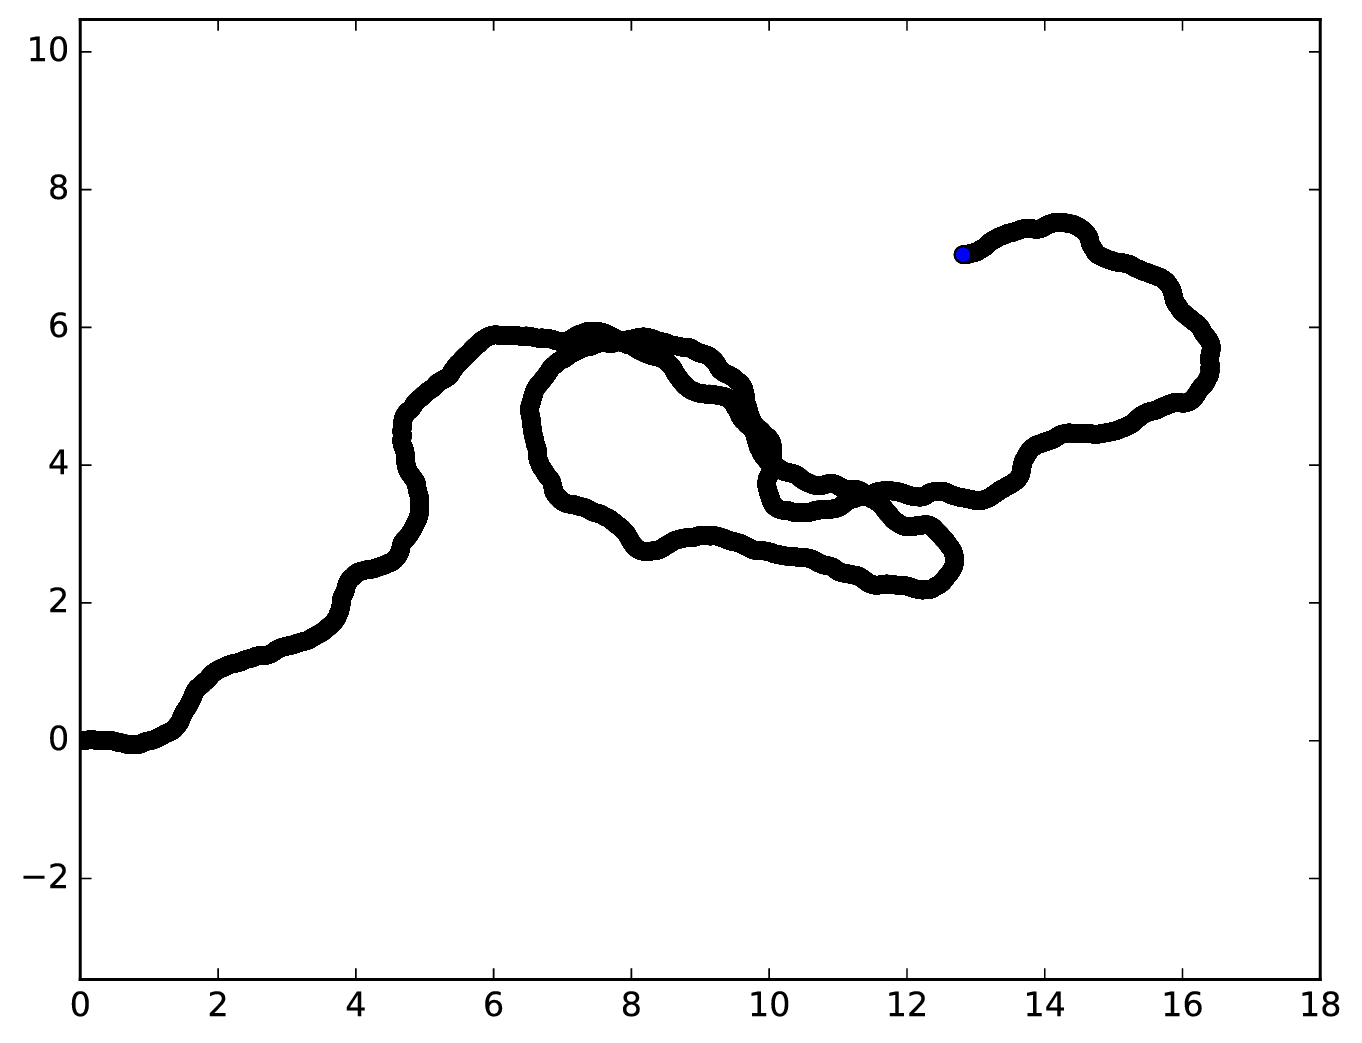
\includegraphics[width=\textwidth]{figures/ch3/synTraj_219_15_60}
			\caption[$A = 15$, $F=60$]{$A = 15$, $F=60$}
			\label{fig:synTraj_219_15_60}
		\end{subfigure}
		~
		\begin{subfigure}[t]{\subImgWmo}
			\centering
			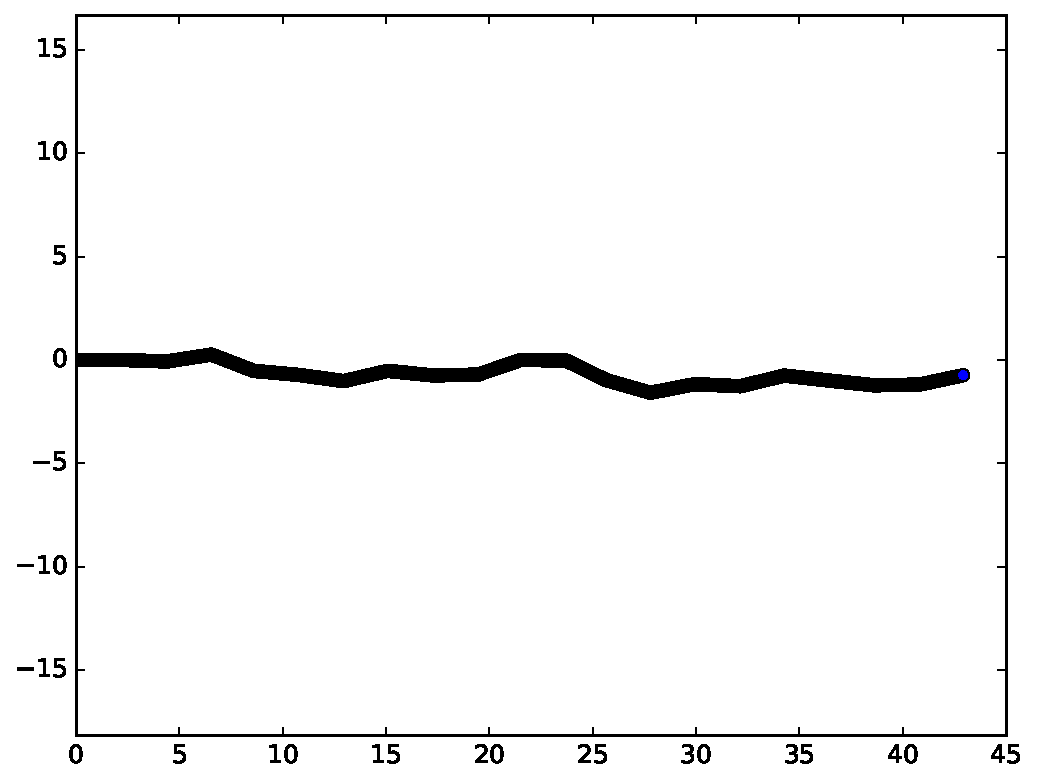
\includegraphics[width=\textwidth]{figures/ch3/synTraj_219_30_1}
			\caption[$A = 30$, $F=1$]{$A = 30$, $F=1$}
			\label{fig:synTraj_219_30_1}
		\end{subfigure}
		~
		\begin{subfigure}[t]{\subImgWmo}
			\centering
			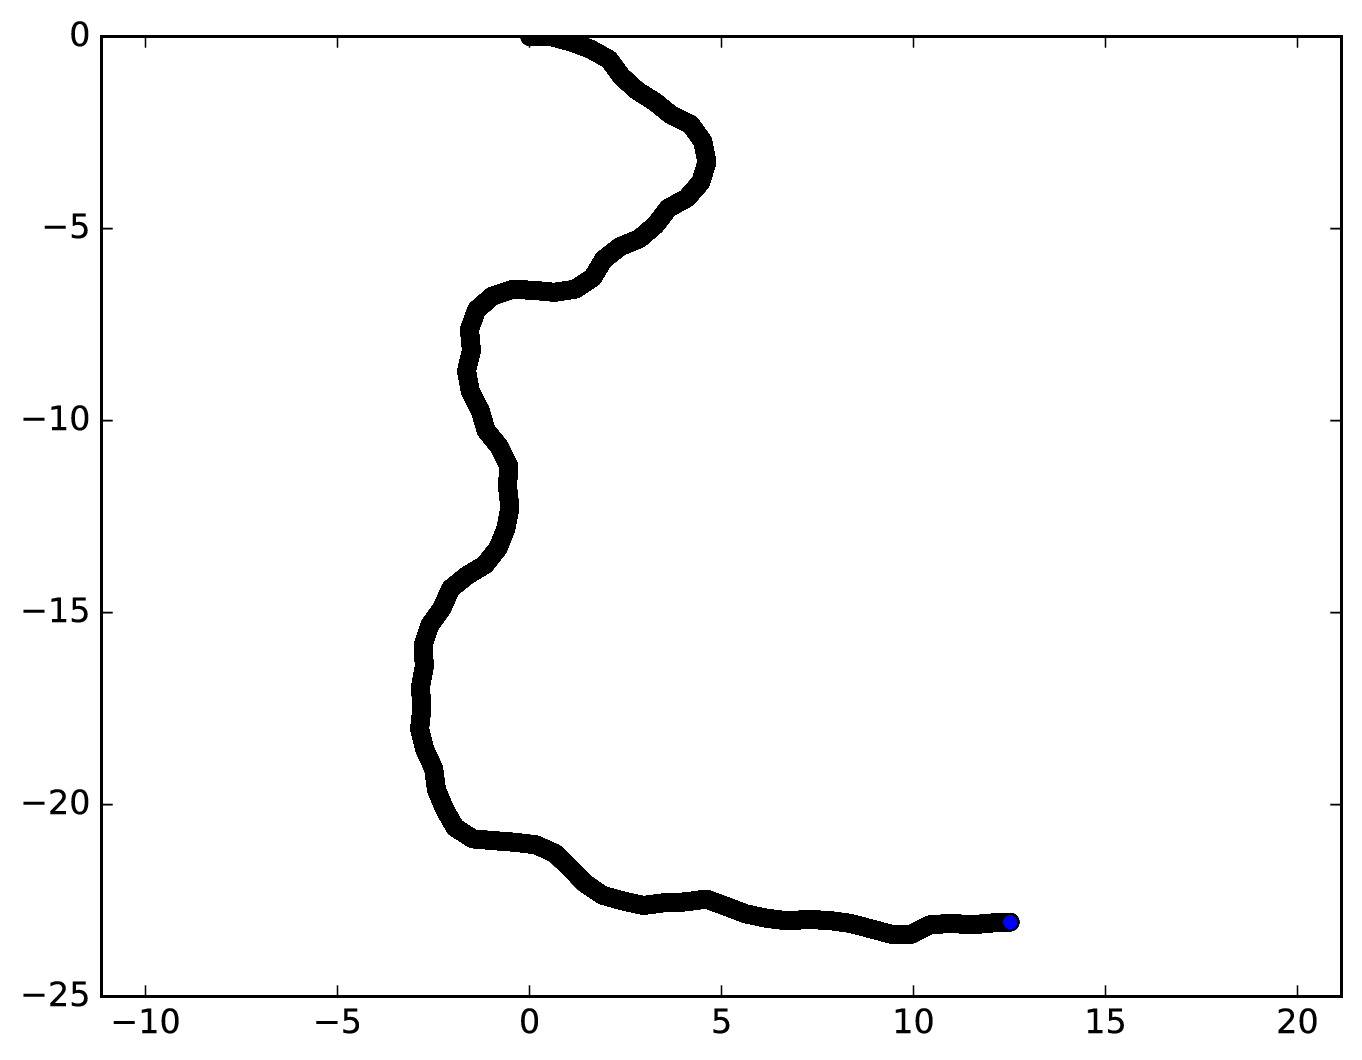
\includegraphics[width=\textwidth]{figures/ch3/synTraj_219_30_4}
			\caption[$A = 30$, $F=4$]{$A = 30$, $F=4$}
			\label{fig:synTraj_219_30_4}
		\end{subfigure}
		~
		\begin{subfigure}[t]{\subImgWmo}
			\centering
			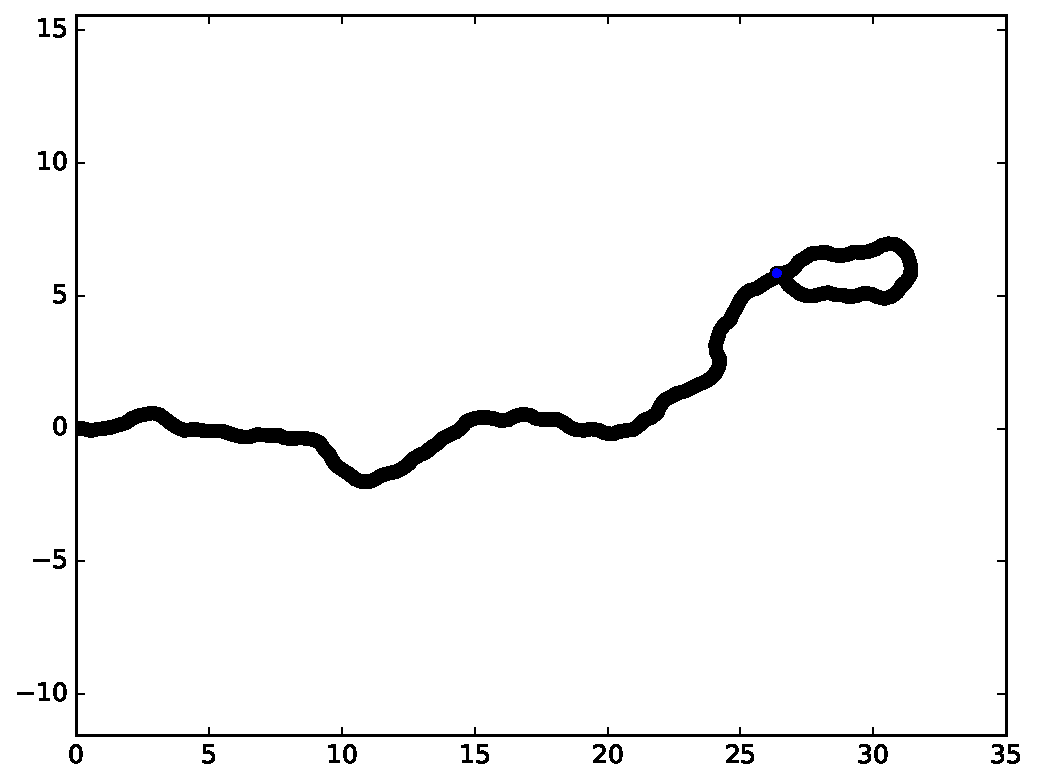
\includegraphics[width=\textwidth]{figures/ch3/synTraj_219_30_8}
			\caption[$A = 30$, $F=8$]{$A = 30$, $F=8$}
			\label{fig:synTraj_219_30_8}
		\end{subfigure}
		~
		\begin{subfigure}[t]{\subImgWmo}
			\centering
			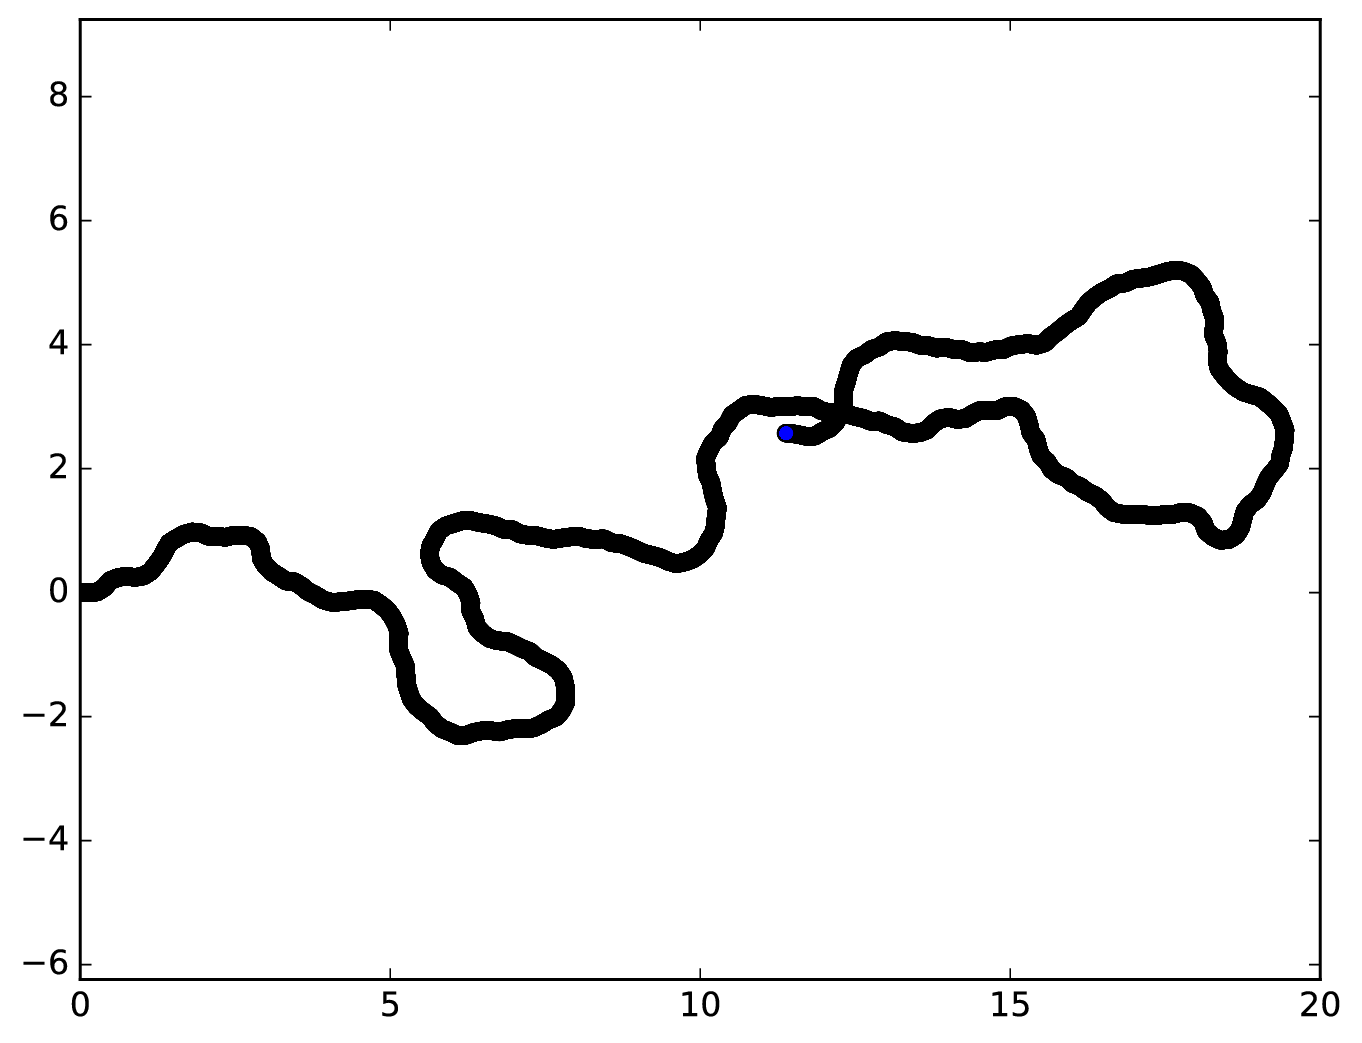
\includegraphics[width=\textwidth]{figures/ch3/synTraj_219_30_16}
			\caption[$A = 30$, $F=16$]{$A = 30$, $F=16$}
			\label{fig:synTraj_219_30_16}
		\end{subfigure}
		~
		\begin{subfigure}[t]{\subImgWmo}
			\centering
			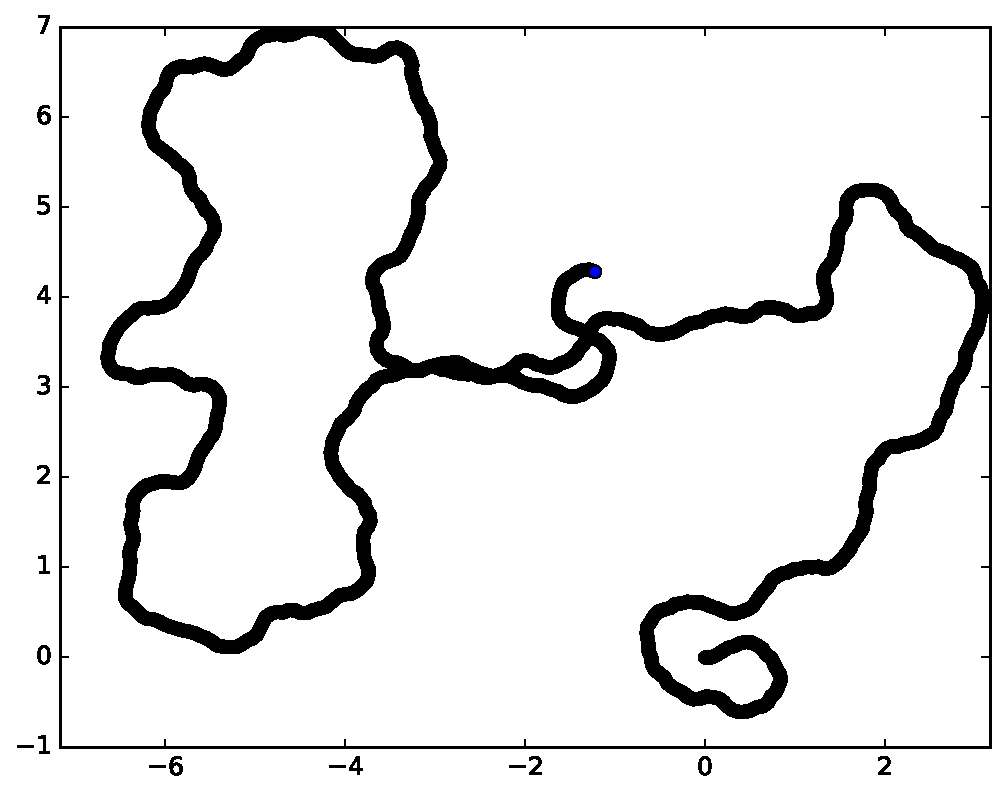
\includegraphics[width=\textwidth]{figures/ch3/synTraj_219_30_32}
			\caption[$A = 30$, $F=32$]{$A = 30$, $F=32$}
			\label{fig:synTraj_219_30_32}
		\end{subfigure}
		~
		\begin{subfigure}[t]{\subImgWmo}
			\centering
			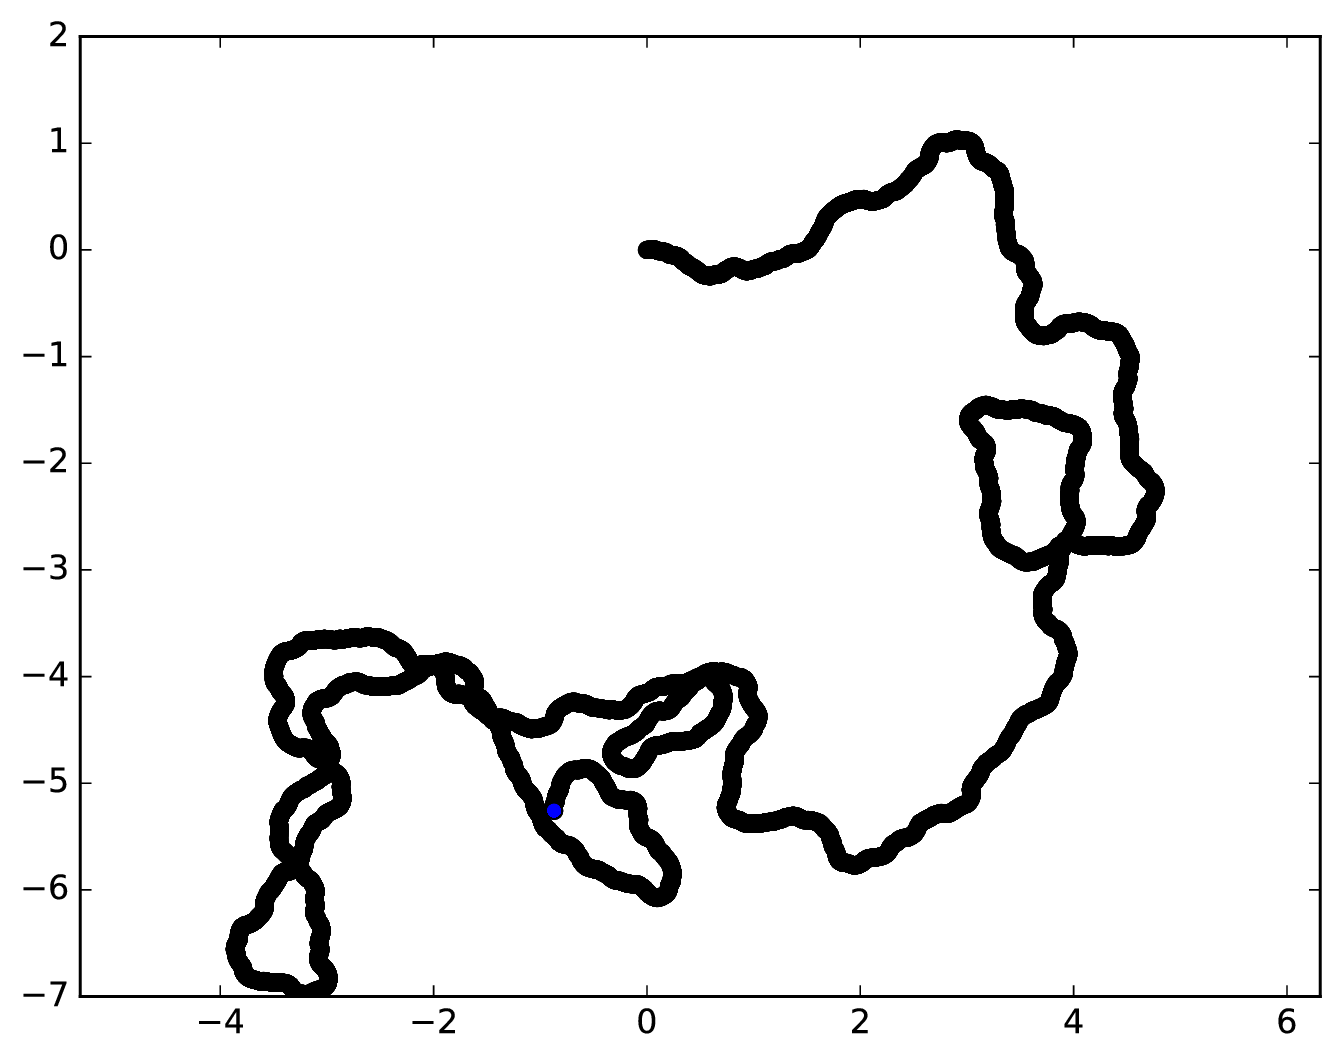
\includegraphics[width=\textwidth]{figures/ch3/synTraj_219_30_60}
			\caption[$A = 30$, $F=60$]{$A = 30$, $F=60$}
			\label{fig:synTraj_219_30_60}
		\end{subfigure}
		\caption[Mouvements générés par notre modèle]{Exemples de trajectoires générées par notre modèle pour un objet de vitesse constante (2,19~cm/s).}
		\label{fig:motion1530}
	\end{figure}
	
    \subsubsection{Impressions subjectives sur les trajectoires}
    \paragraph{Mouvement pseudo-autocorrélé.}
    On notera (notamment sur la figure~\ref{fig:motion1530}, et dans une moindre mesure sur les autres) que quand les valeurs de $A$ ou $F$ sont faibles, ou \emph{a fortiori} quand les deux le sont, le mouvement semble présenter une certaine régularité, au point peut-être de donner l'illusion d'être autocorrélé. La figure~\ref{fig:synTraj_219_45_1}, malgré sa valeur de $A$ relativement élevée, en fournit un exemple.
    
    Cette observation est intéressante en ce que ce modèle conçu pour les objets markoviens peut fournir une approximation du mouvement autocorrélé qui, dans certains cas, peut être suffisante. C'est particulièremnt vrai sur une fenêtre temporelle plus restreinte, limitée à quelques secondes tout au plus --- mais une telle fenêtre peut être trop courte pour certaines applications.
    
    À défaut d'être réellement autocorrélés, les mouvements générés par ces conditions (que l'on peut résumer par une valeur de $A \times F$ faible) engendrent des trajectoires suffisamment \og régulières \fg{} pour être relativement prévisibles à court terme (sur une ou deux secondes). Nous reviendrons plus loin sur l'importance de la prévisibilité pour une tâche de sélection. Contentons-nous pour le moment de remarquer qu'un objet dont les changements de direction sont rares et/ou de faible amplitude tend à avoir une trajectoire relativement \og lisse \fg{} et, de fait, prévisible.


	\begin{figure}[htb]
		\begin{subfigure}[t]{\subImgWmo}
			\centering
			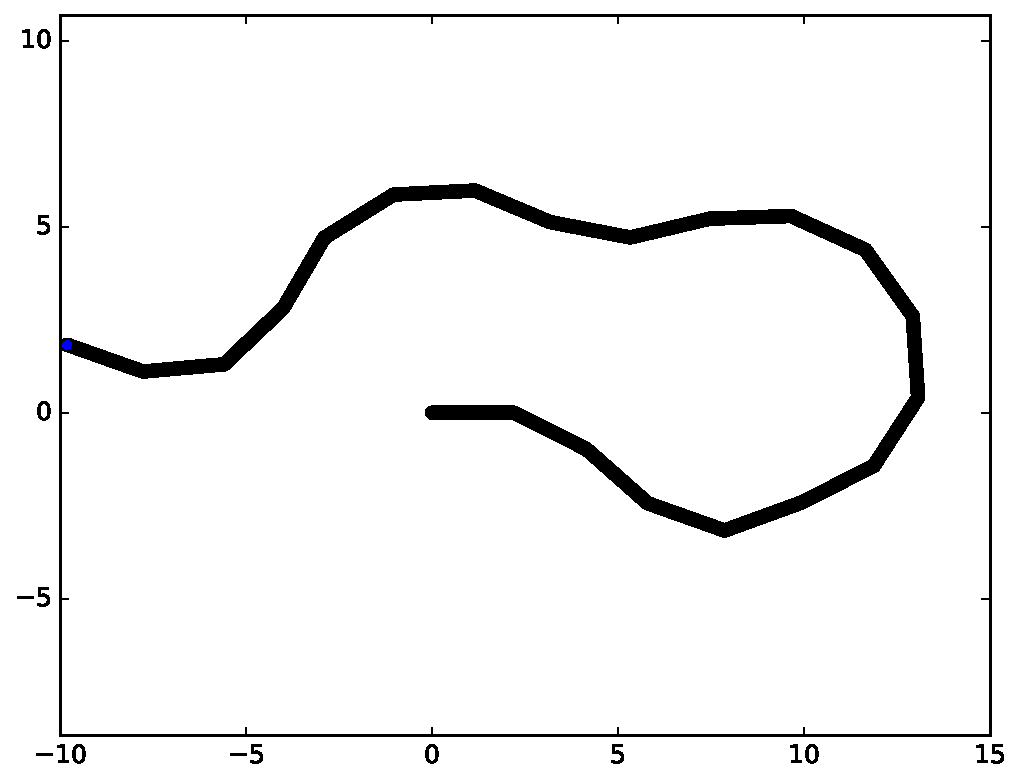
\includegraphics[width=\textwidth]{figures/ch3/synTraj_219_45_1}
			\caption[$A = 45$, $F=1$]{$A = 45$, $F=1$}
			\label{fig:synTraj_219_45_1}
		\end{subfigure}
		~
		\begin{subfigure}[t]{\subImgWmo}
			\centering
			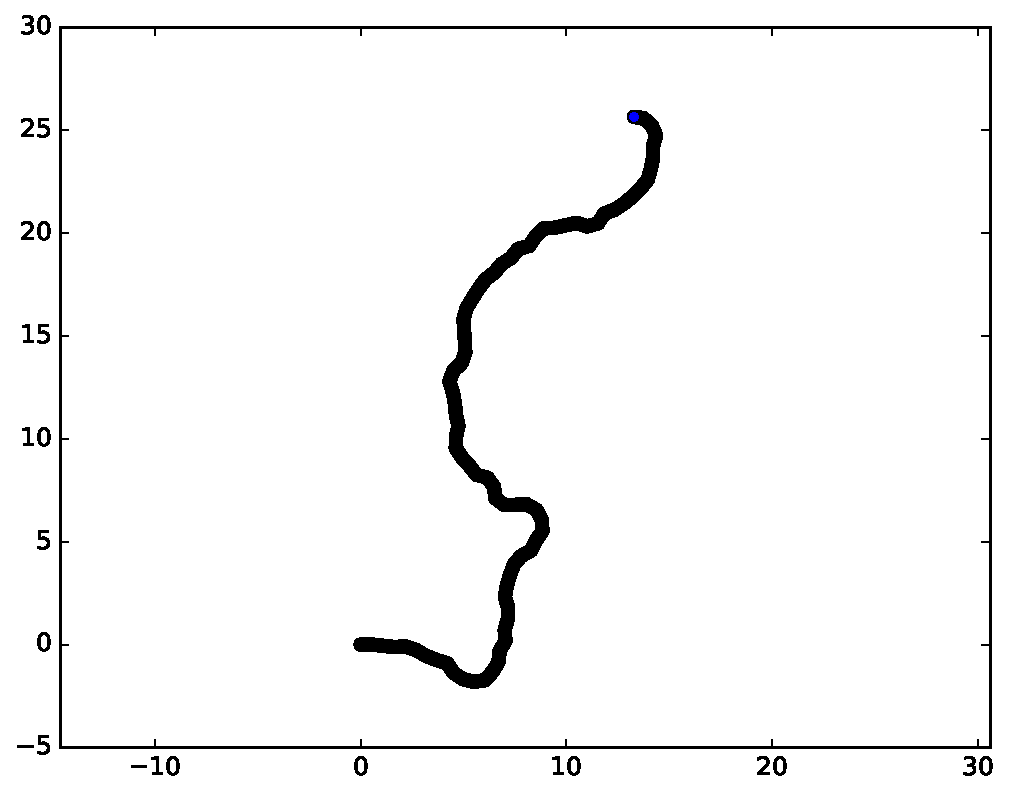
\includegraphics[width=\textwidth]{figures/ch3/synTraj_219_45_4}
			\caption[$A = 45$, $F=4$]{$A = 45$, $F=4$}
			\label{fig:synTraj_219_45_4}
		\end{subfigure}
		~
		\begin{subfigure}[t]{\subImgWmo}
			\centering
			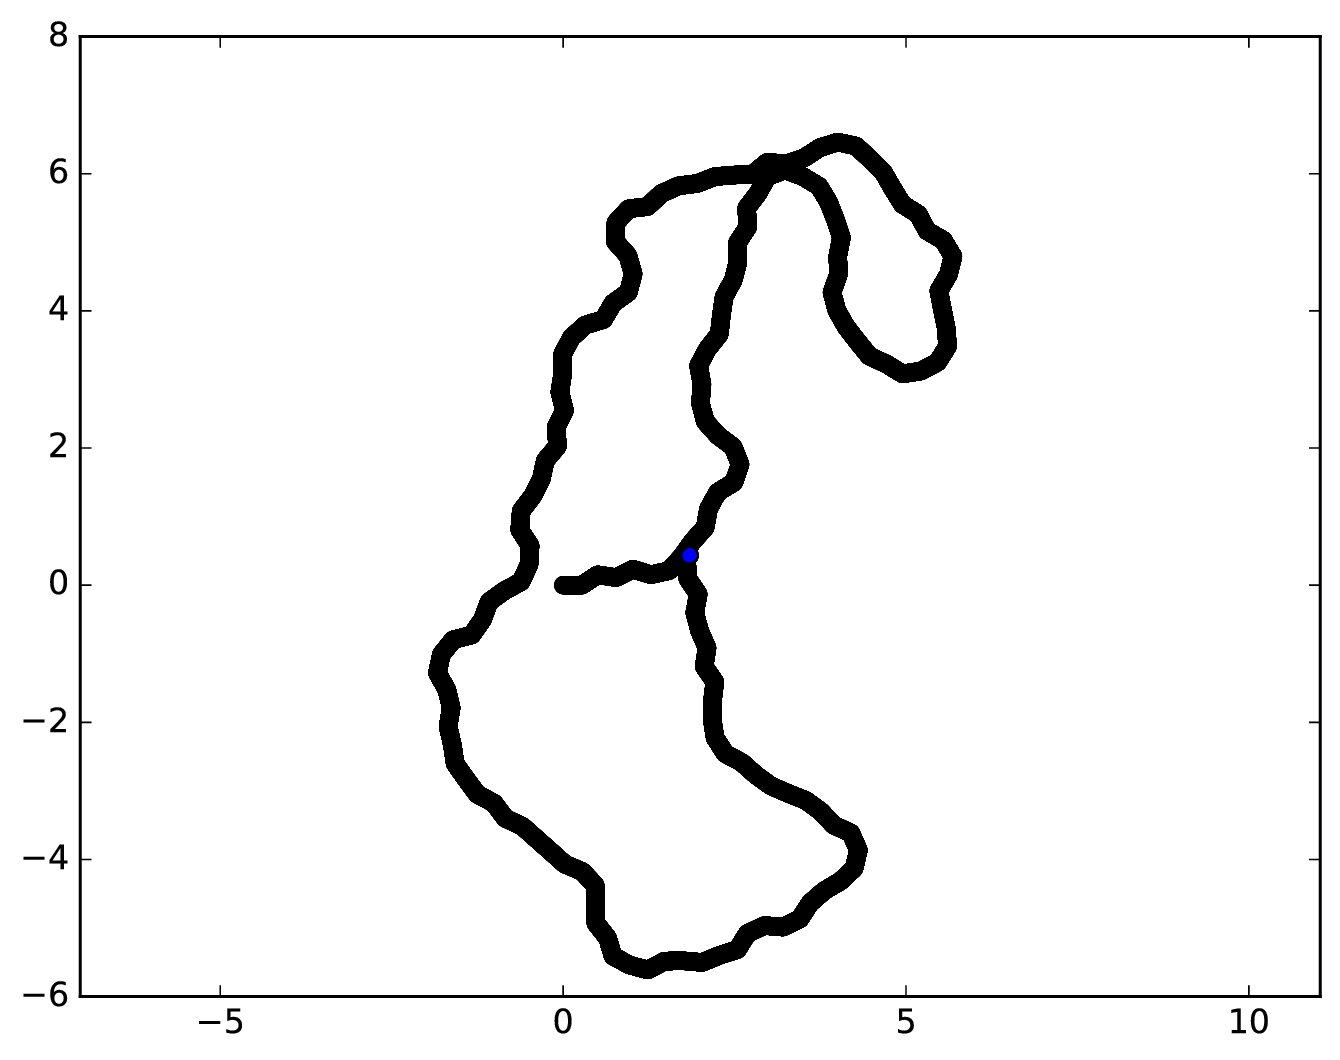
\includegraphics[width=\textwidth]{figures/ch3/synTraj_219_45_8}
			\caption[$A = 45$, $F=8$]{$A = 45$, $F=8$}
			\label{fig:synTraj_219_45_8}
		\end{subfigure}
		~
		\begin{subfigure}[t]{\subImgWmo}
			\centering
			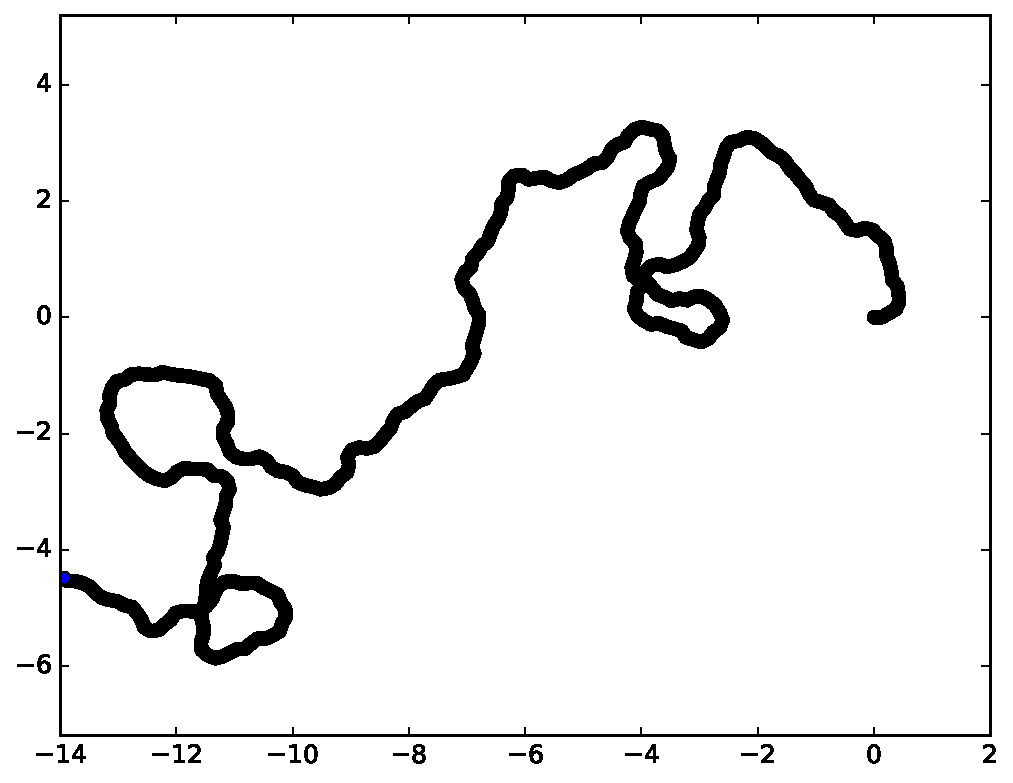
\includegraphics[width=\textwidth]{figures/ch3/synTraj_219_45_16}
			\caption[$A = 45$, $F=16$]{$A = 45$, $F=16$}
			\label{fig:synTraj_219_45_16}
		\end{subfigure}
		~
		\begin{subfigure}[t]{\subImgWmo}
			\centering
			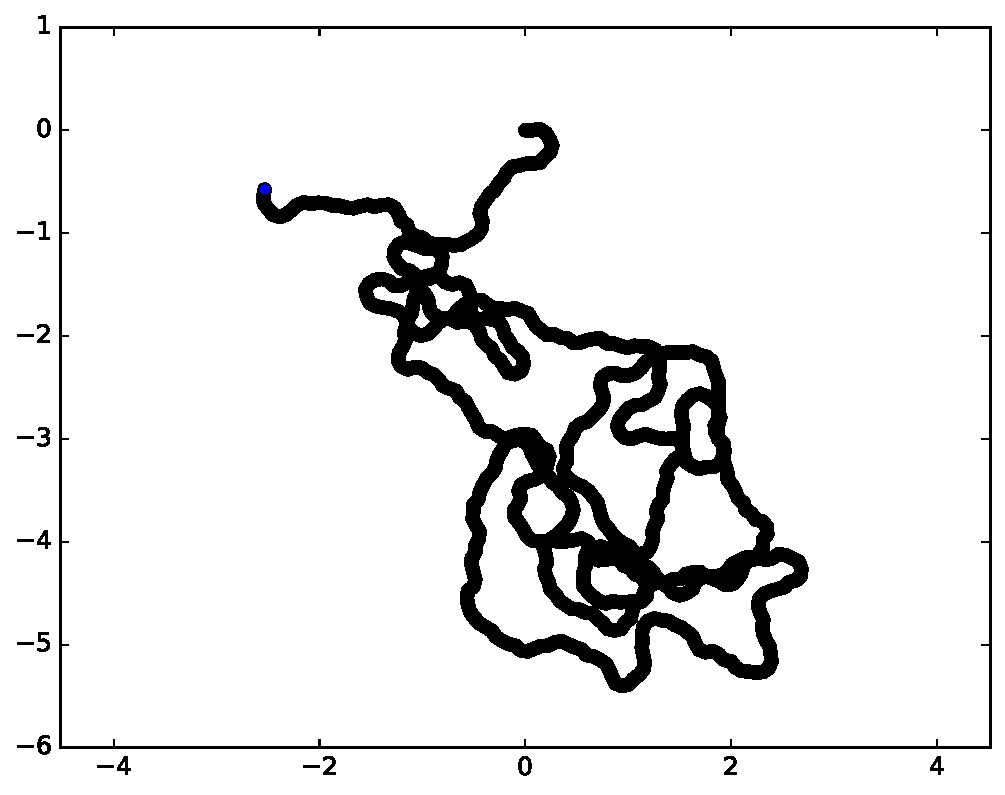
\includegraphics[width=\textwidth]{figures/ch3/synTraj_219_45_32}
			\caption[$A = 45$, $F=32$]{$A = 45$, $F=32$}
			\label{fig:synTraj_219_45_32}
		\end{subfigure}
		~
		\begin{subfigure}[t]{\subImgWmo}
			\centering
			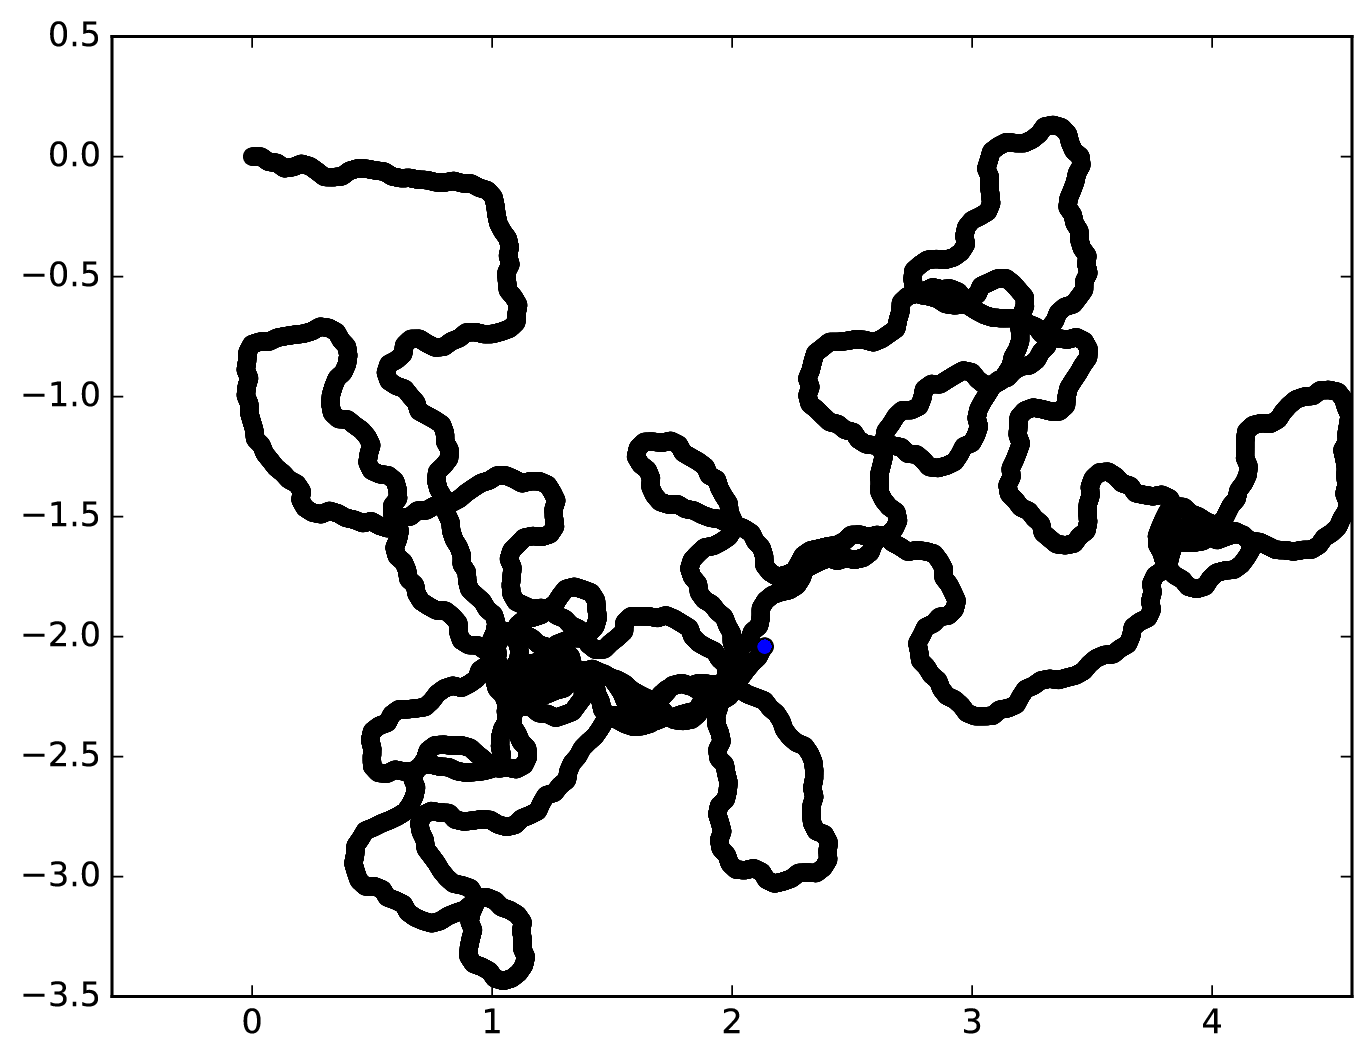
\includegraphics[width=\textwidth]{figures/ch3/synTraj_219_45_60}
			\caption[$A = 45$, $F=60$]{$A = 45$, $F=60$}
			\label{fig:synTraj_219_45_60}
		\end{subfigure}
		~
		\begin{subfigure}[t]{\subImgWmo}
			\centering
			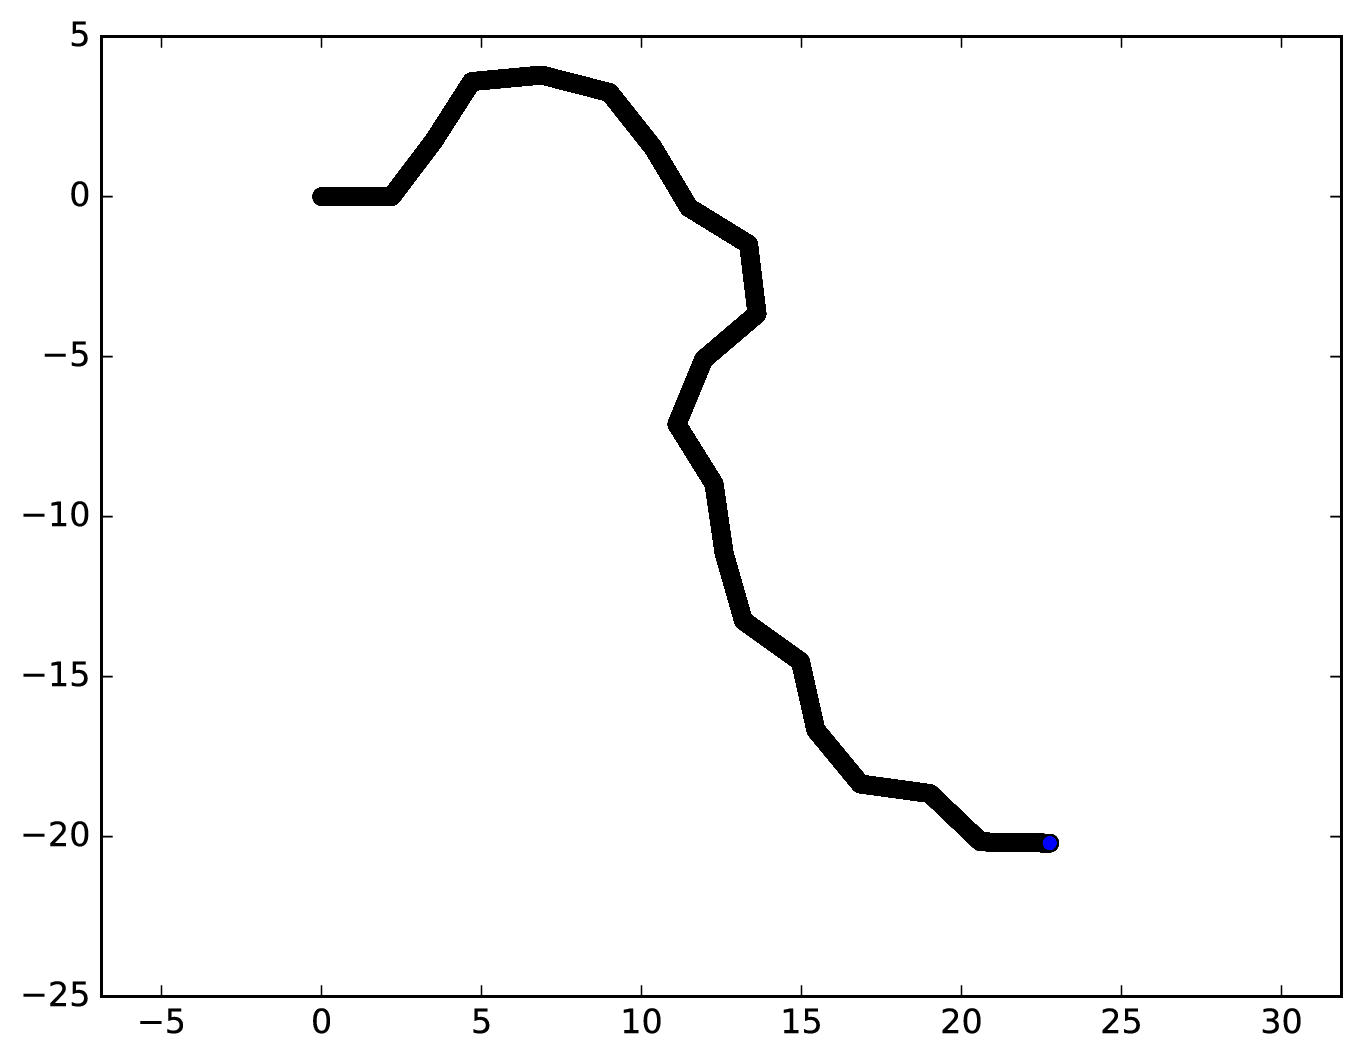
\includegraphics[width=\textwidth]{figures/ch3/synTraj_219_60_1}
			\caption[$A = 60$, $F=1$]{$A = 60$, $F=1$}
			\label{fig:synTraj_219_60_1}
		\end{subfigure}
		~
		\begin{subfigure}[t]{\subImgWmo}
			\centering
			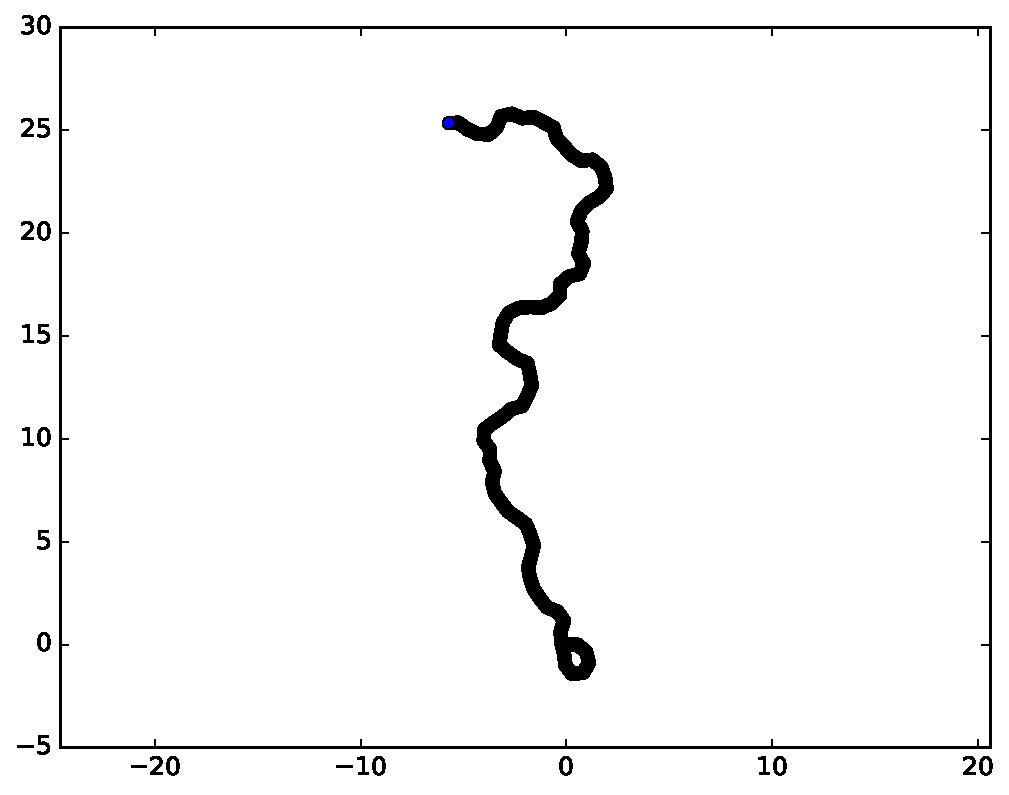
\includegraphics[width=\textwidth]{figures/ch3/synTraj_219_60_4}
			\caption[$A = 60$, $F=4$]{$A = 60$, $F=4$}
			\label{fig:synTraj_219_60_4}
		\end{subfigure}
		~
		\begin{subfigure}[t]{\subImgWmo}
			\centering
			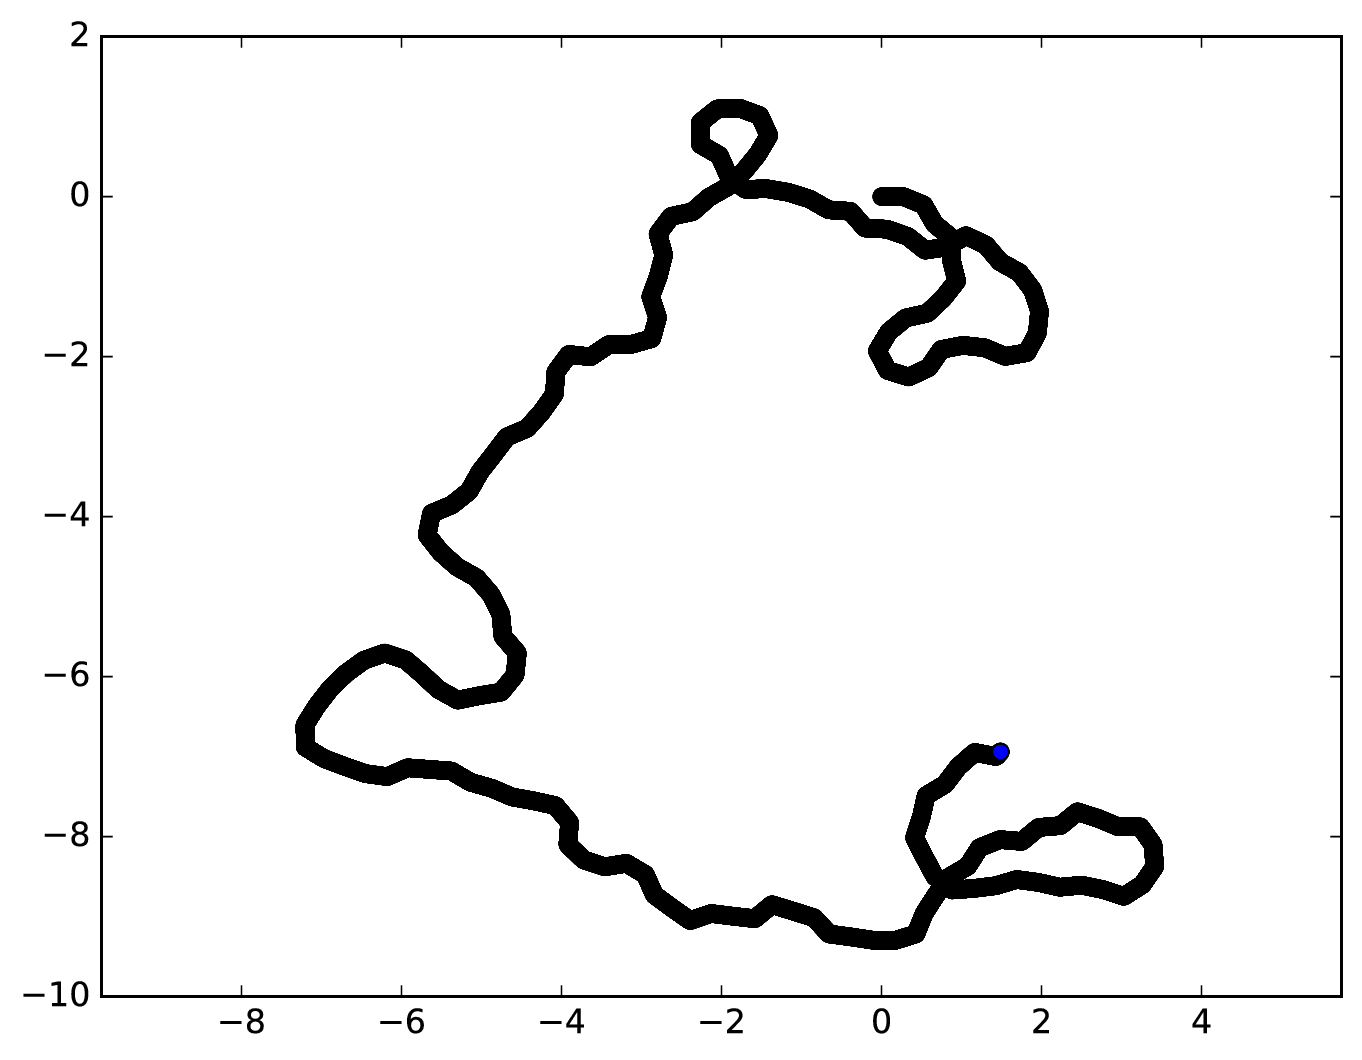
\includegraphics[width=\textwidth]{figures/ch3/synTraj_219_60_8}
			\caption[$A = 60$, $F=8$]{$A = 60$, $F=8$}
			\label{fig:synTraj_219_60_8}
		\end{subfigure}
		~
		\begin{subfigure}[t]{\subImgWmo}
			\centering
			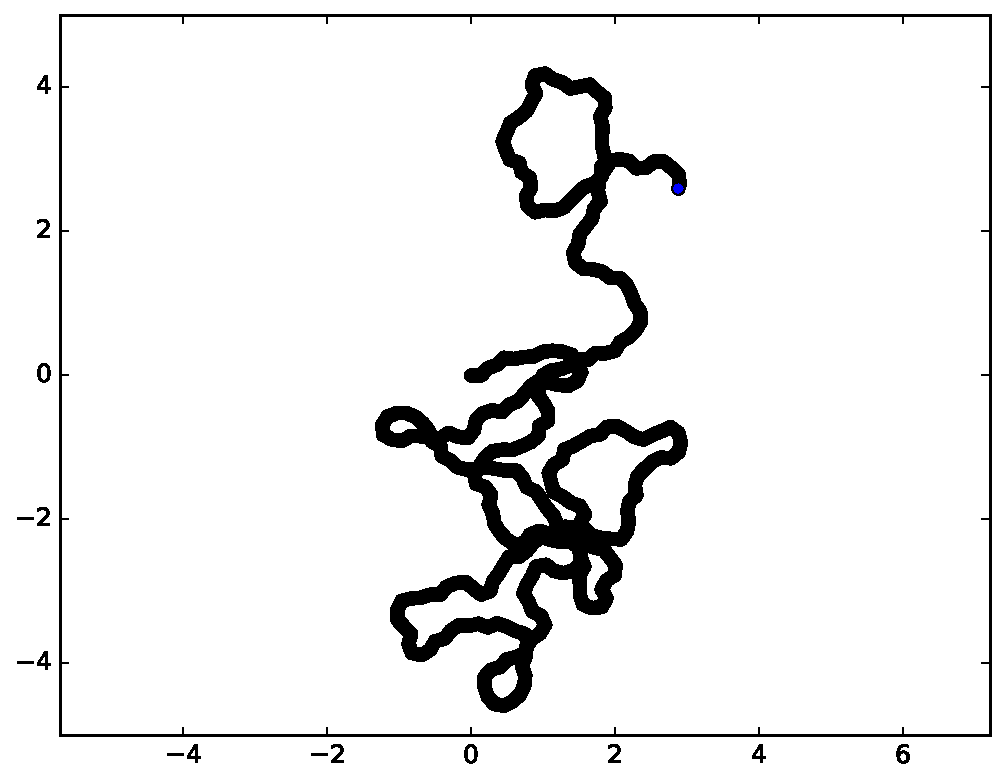
\includegraphics[width=\textwidth]{figures/ch3/synTraj_219_60_16}
			\caption[$A = 60$, $F=16$]{$A = 60$, $F=16$}
			\label{fig:synTraj_219_60_16}
		\end{subfigure}
		~
		\begin{subfigure}[t]{\subImgWmo}
			\centering
			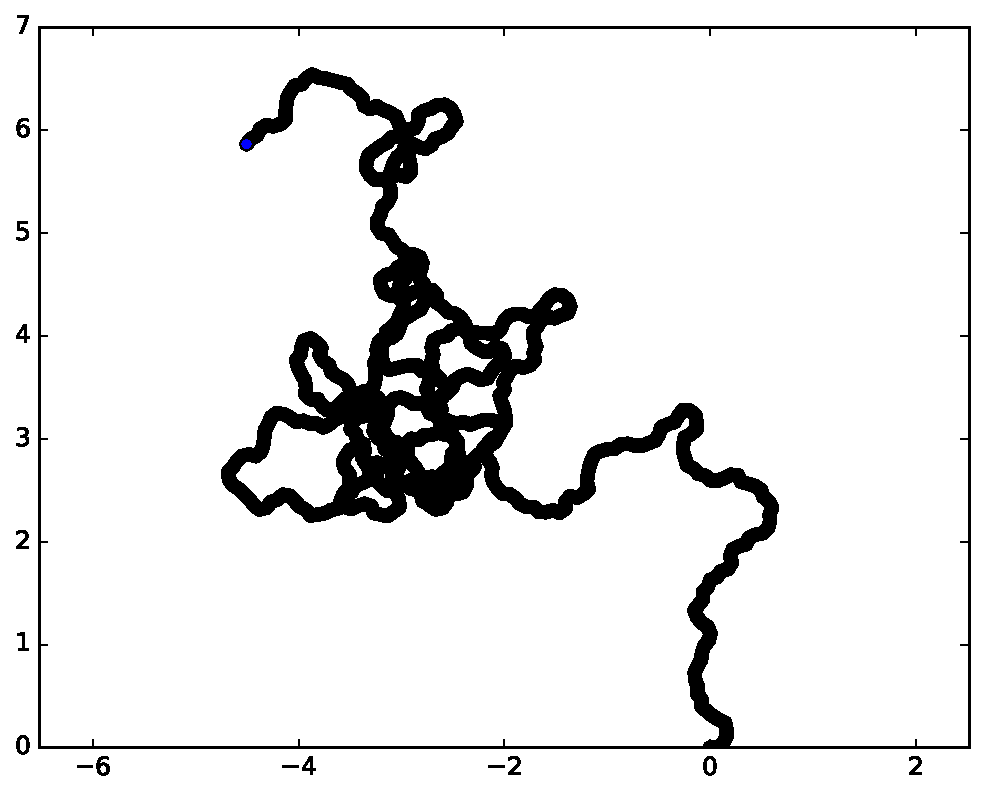
\includegraphics[width=\textwidth]{figures/ch3/synTraj_219_60_32}
			\caption[$A = 60$, $F=32$]{$A = 60$, $F=32$}
			\label{fig:synTraj_219_60_32}
		\end{subfigure}
		~
		\begin{subfigure}[t]{\subImgWmo}
			\centering
			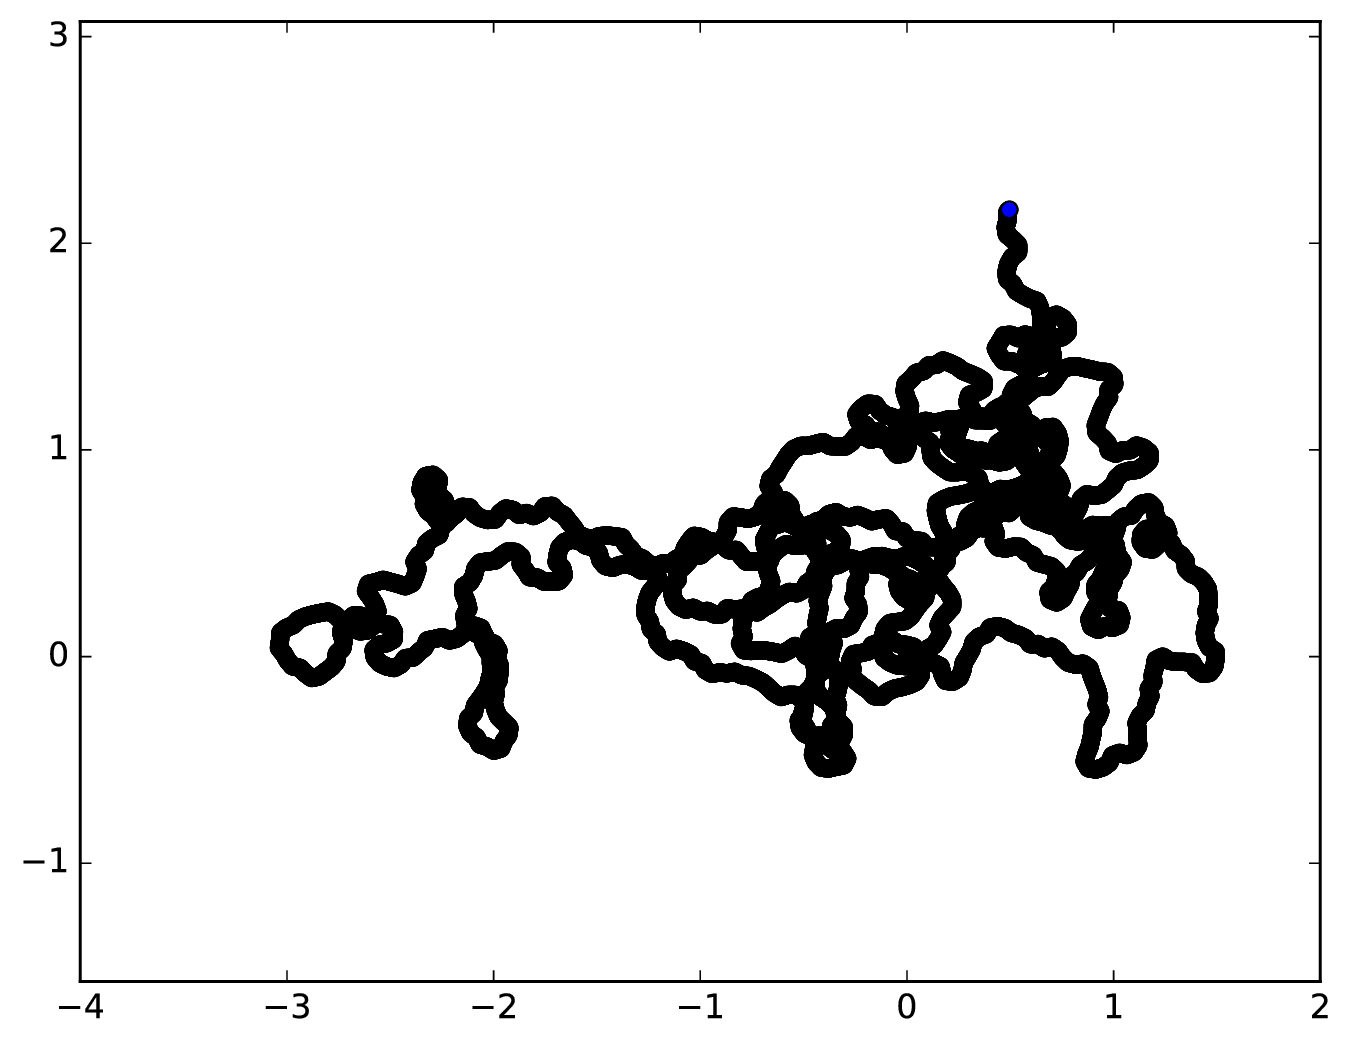
\includegraphics[width=\textwidth]{figures/ch3/synTraj_219_60_60}
			\caption[$A = 60$, $F=60$]{$A = 60$, $F=60$}
			\label{fig:synTraj_219_60_60}
		\end{subfigure}
		\caption[Mouvements générés par notre modèle -- II]{Exemples de trajectoires générées par notre modèle pour un objet de vitesse constante (2,19~cm/s).}
		\label{fig:motion4560}
	\end{figure}
	
	
	\begin{figure}[htb]
		\begin{subfigure}[t]{\subImgWmo}
			\centering
			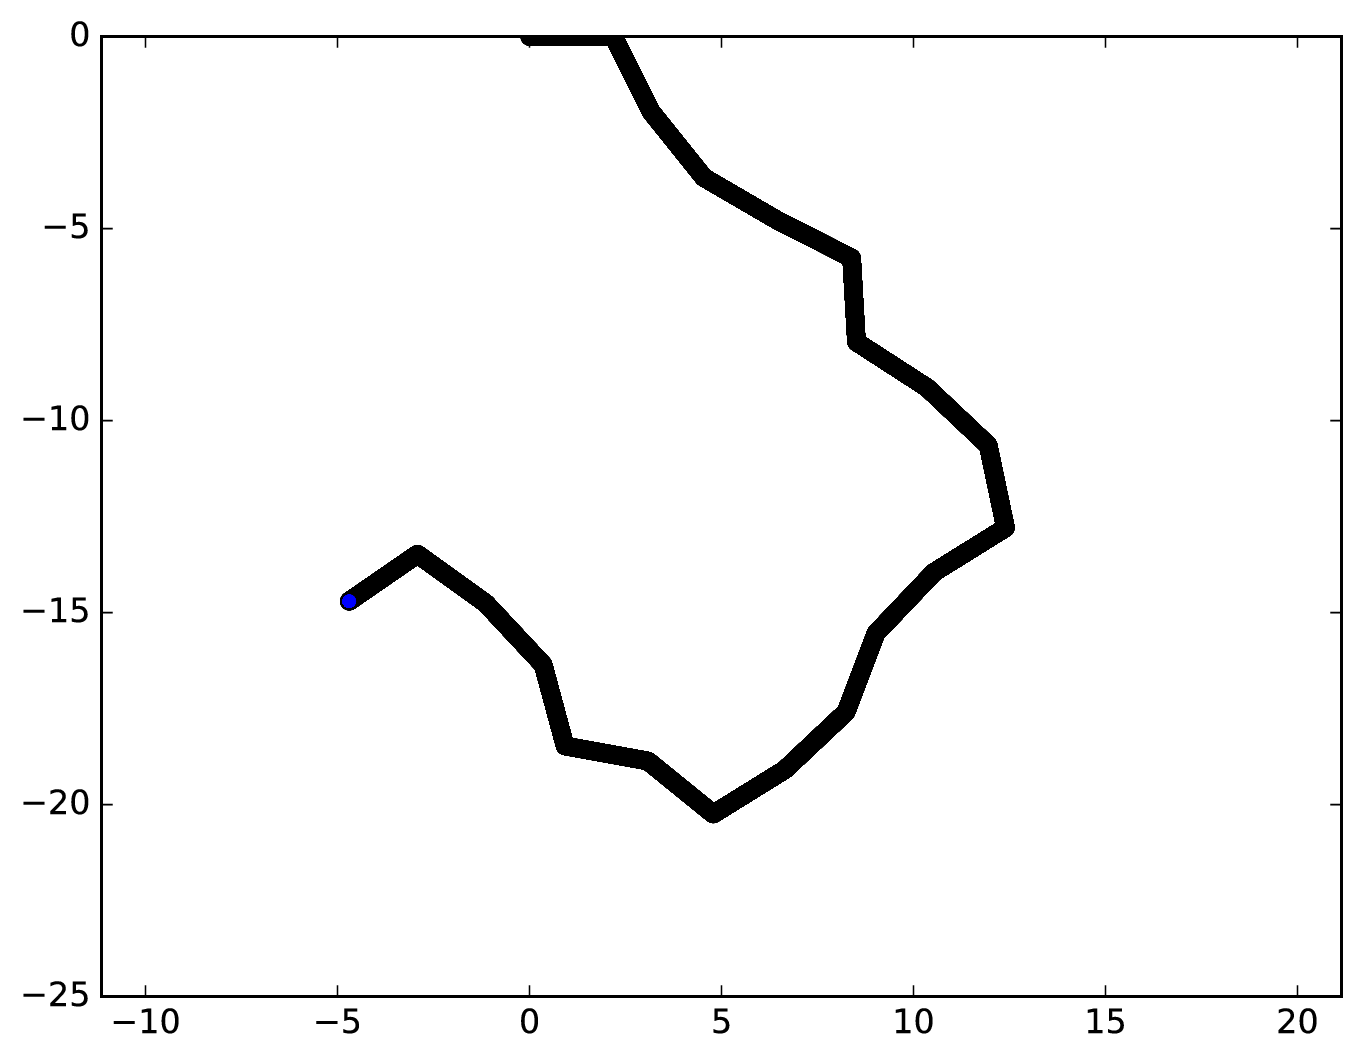
\includegraphics[width=\textwidth]{figures/ch3/synTraj_219_75_1}
			\caption[$A = 75$, $F=1$]{$A = 75$, $F=1$}
			\label{fig:synTraj_219_75_1}
		\end{subfigure}
		~
		\begin{subfigure}[t]{\subImgWmo}
			\centering
			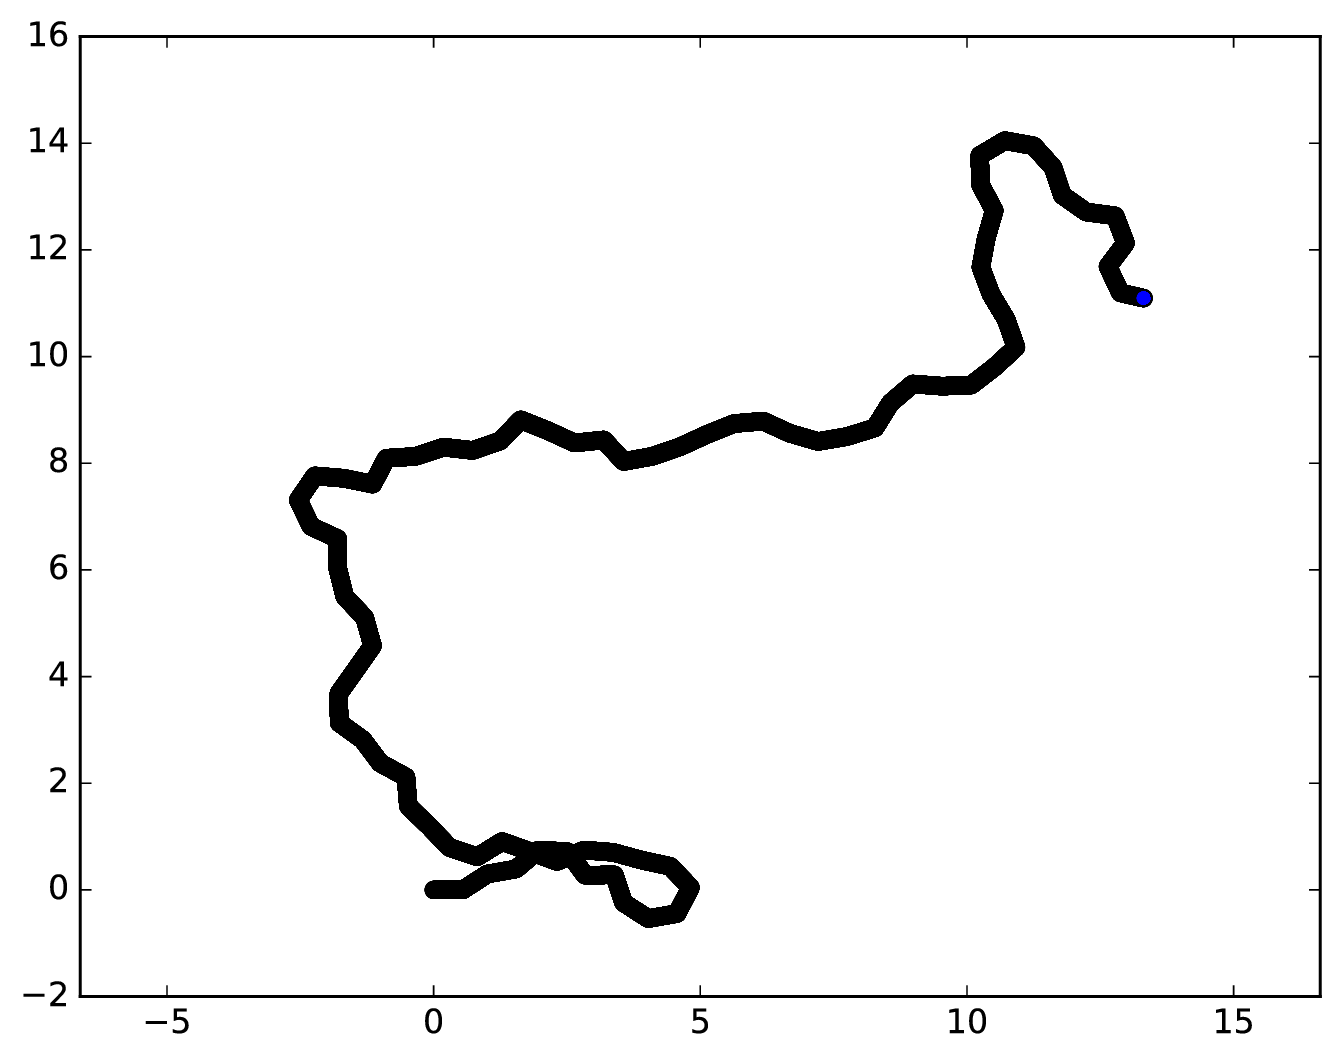
\includegraphics[width=\textwidth]{figures/ch3/synTraj_219_75_4}
			\caption[$A = 75$, $F=4$]{$A = 75$, $F=4$}
			\label{fig:synTraj_219_75_4}
		\end{subfigure}
		~
		\begin{subfigure}[t]{\subImgWmo}
			\centering
			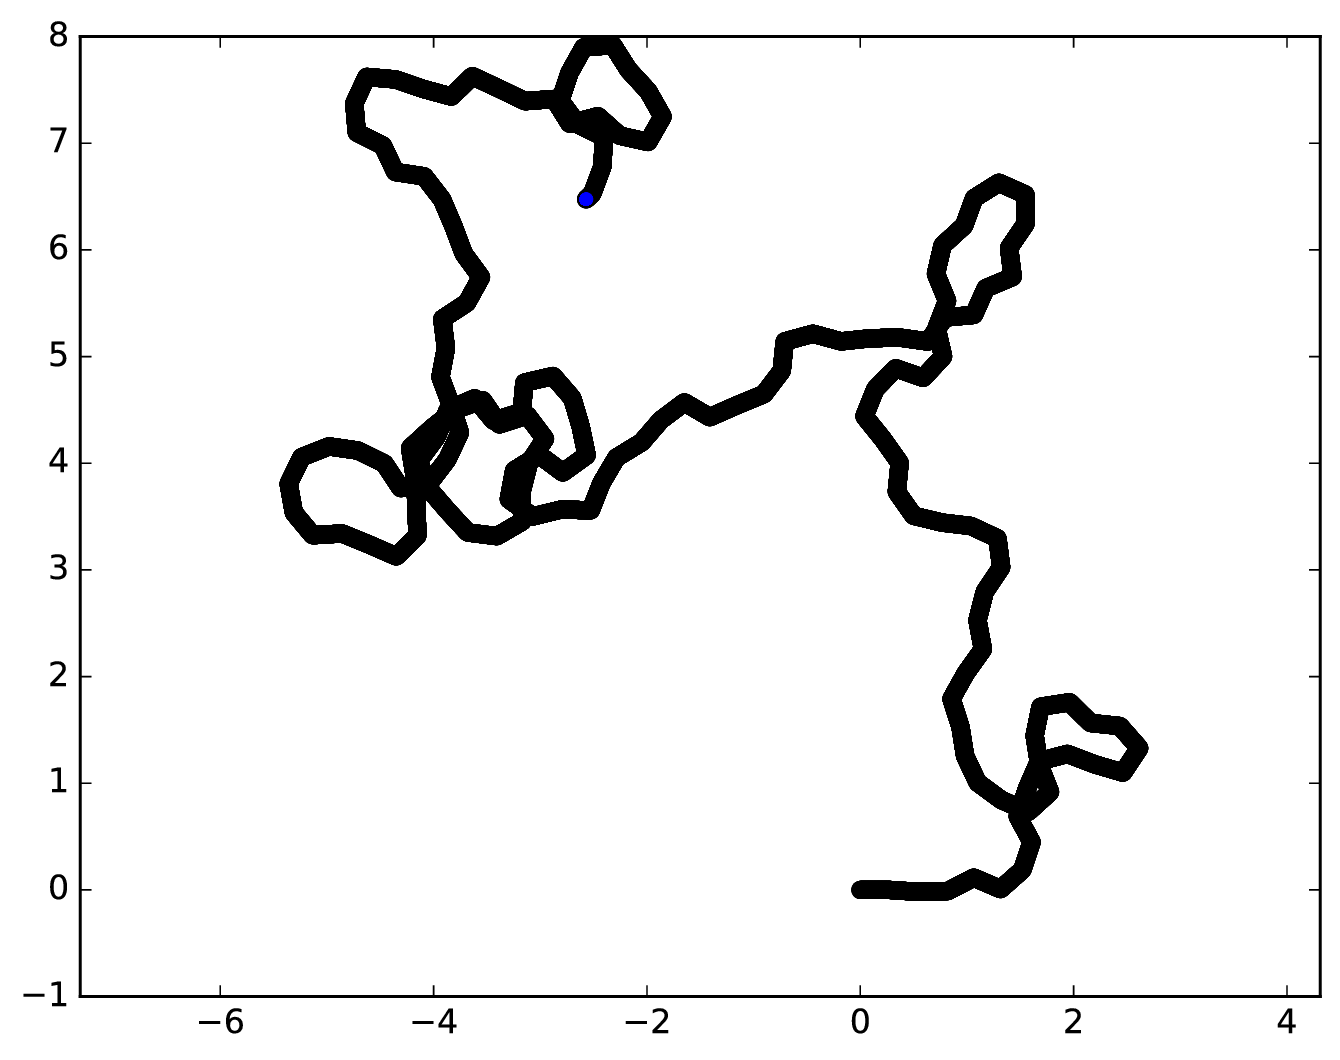
\includegraphics[width=\textwidth]{figures/ch3/synTraj_219_75_8}
			\caption[$A = 75$, $F=8$]{$A = 75$, $F=8$}
			\label{fig:synTraj_219_75_8}
		\end{subfigure}
		~
		\begin{subfigure}[t]{\subImgWmo}
			\centering
			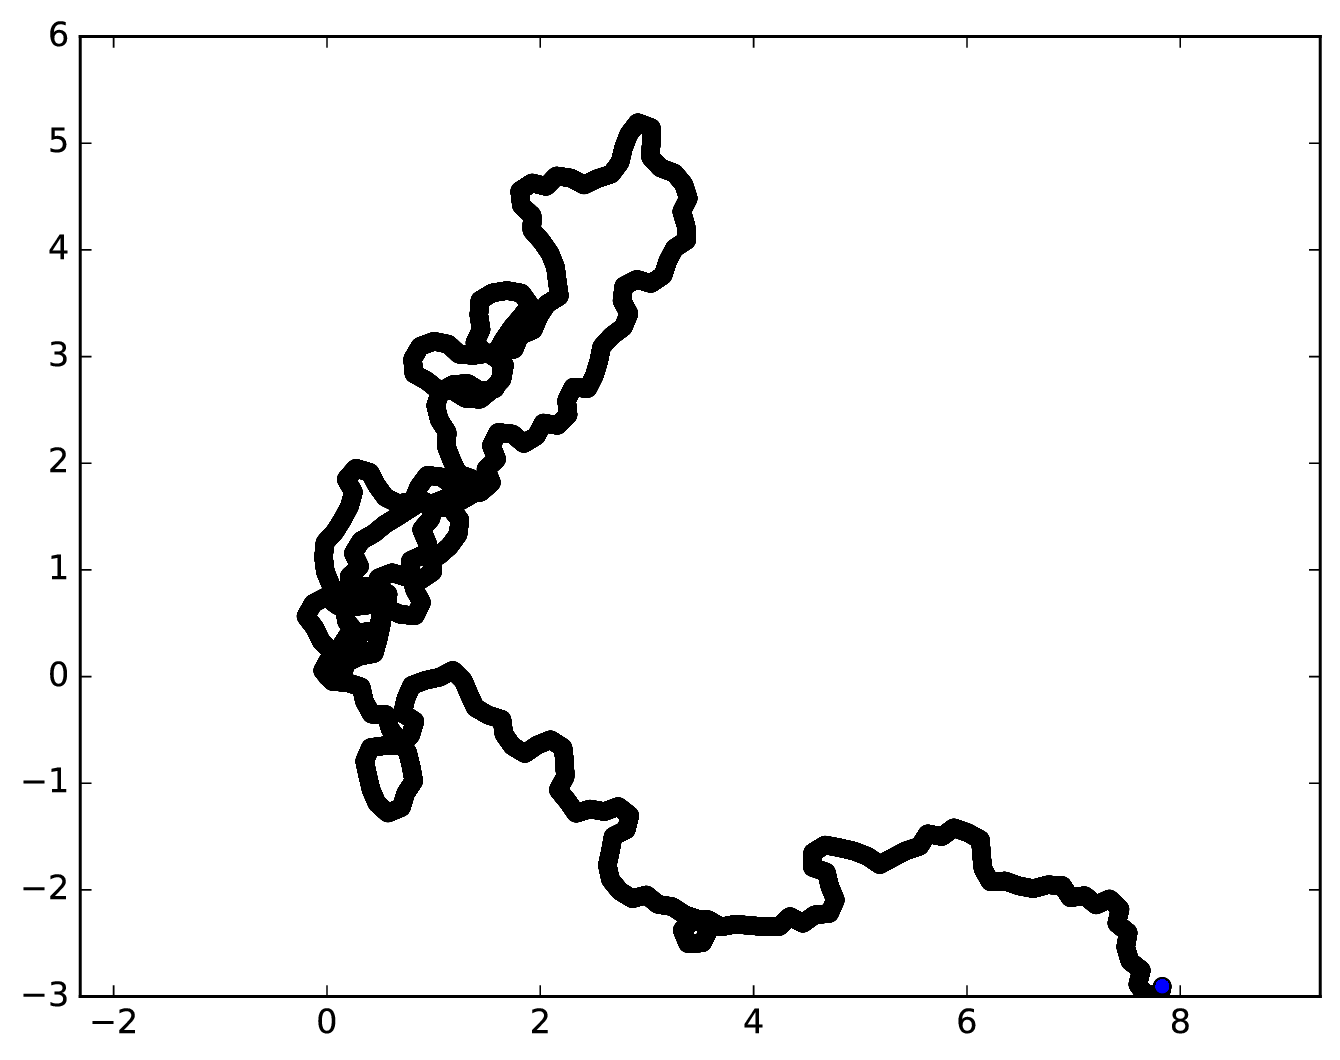
\includegraphics[width=\textwidth]{figures/ch3/synTraj_219_75_16}
			\caption[$A = 75$, $F=16$]{$A = 75$, $F=16$}
			\label{fig:synTraj_219_75_16}
		\end{subfigure}
		~
		\begin{subfigure}[t]{\subImgWmo}
			\centering
			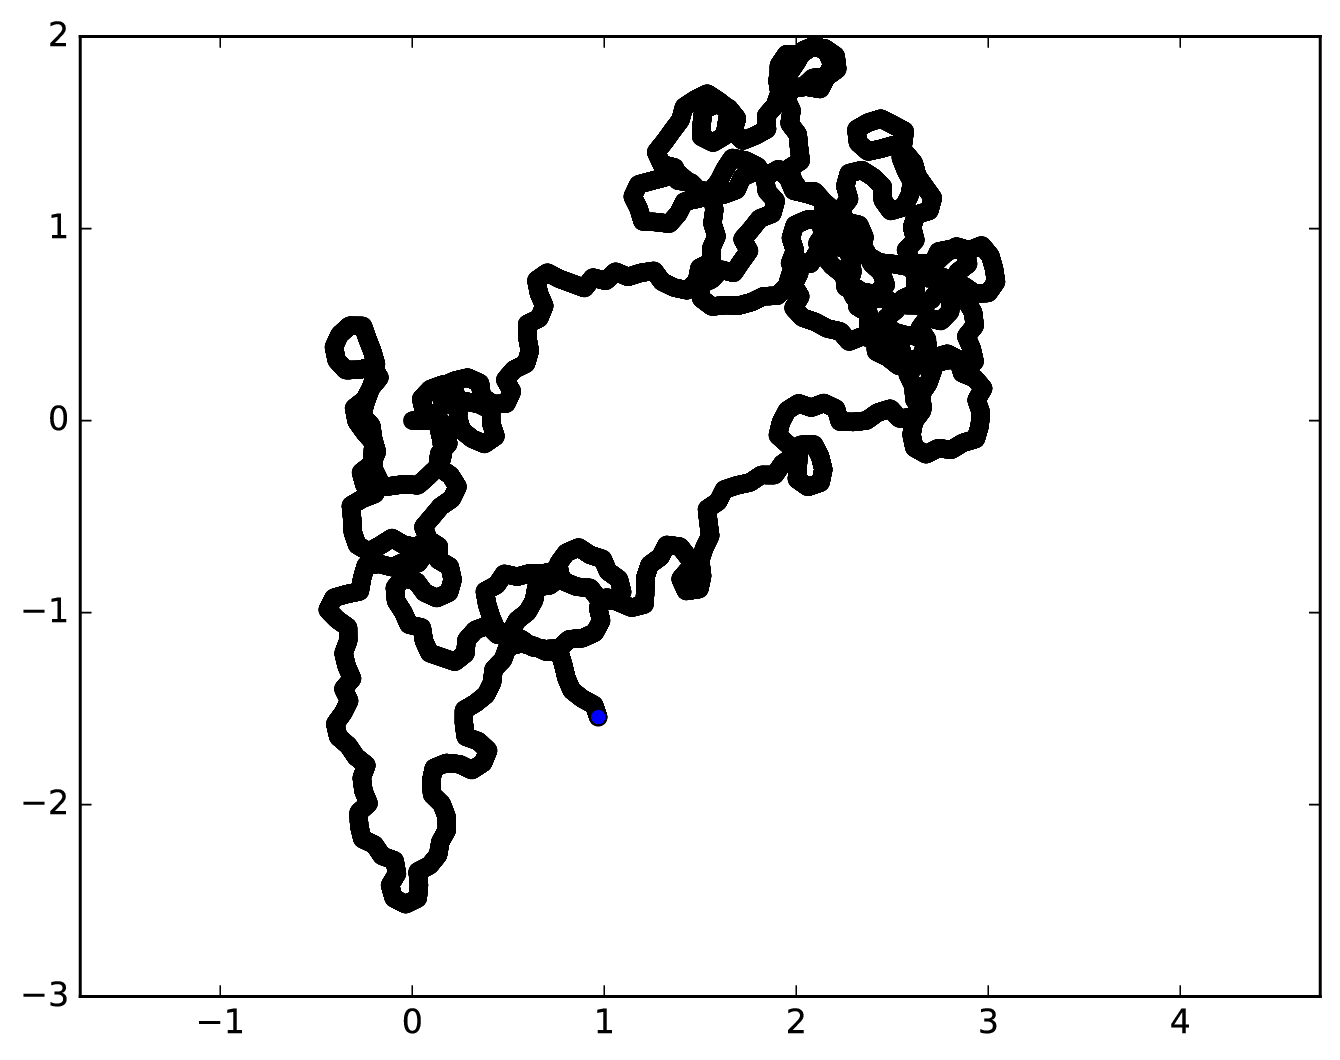
\includegraphics[width=\textwidth]{figures/ch3/synTraj_219_75_32}
			\caption[$A = 75$, $F=32$]{$A = 75$, $F=32$}
			\label{fig:synTraj_219_75_32}
		\end{subfigure}
		~
		\begin{subfigure}[t]{\subImgWmo}
			\centering
			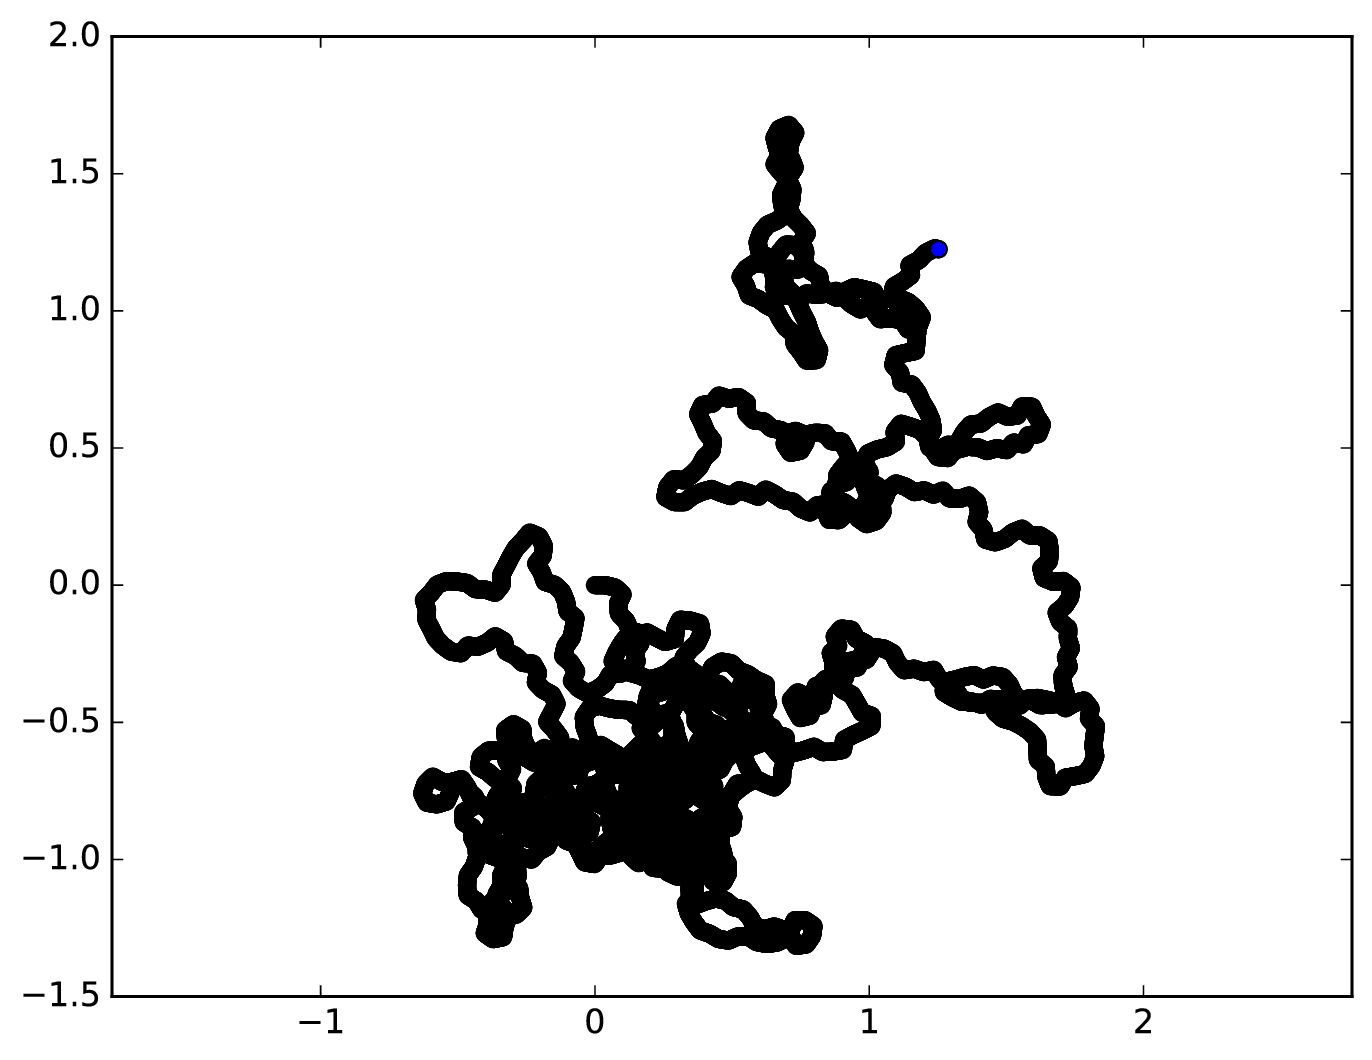
\includegraphics[width=\textwidth]{figures/ch3/synTraj_219_75_60}
			\caption[$A = 75$, $F=60$]{$A = 75$, $F=60$}
			\label{fig:synTraj_219_75_60}
		\end{subfigure}
		~
		\begin{subfigure}[t]{\subImgWmo}
			\centering
			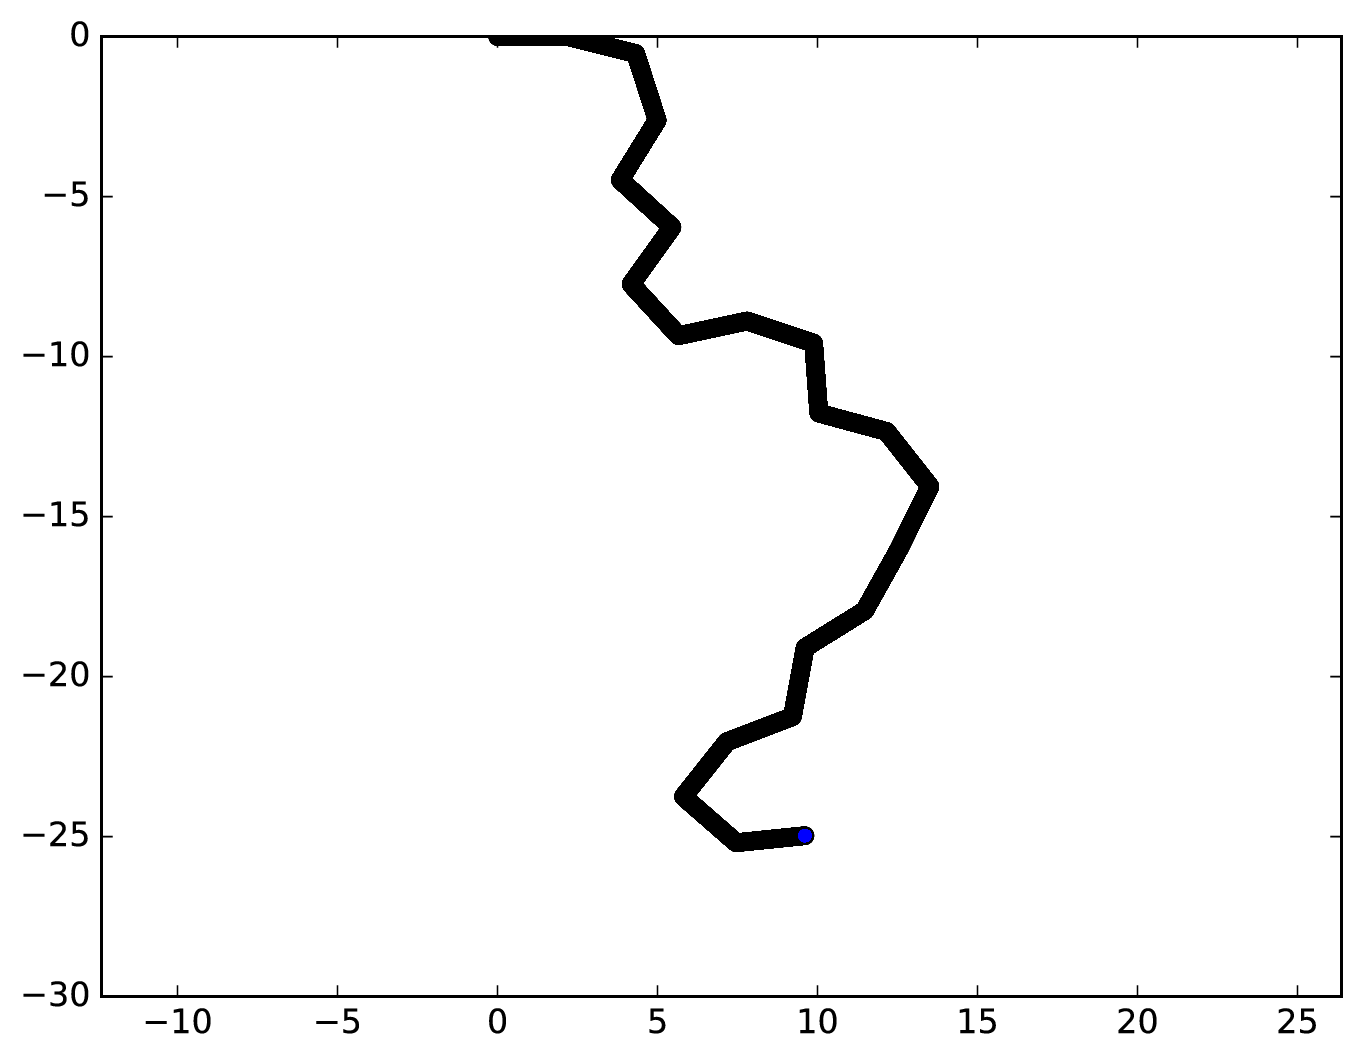
\includegraphics[width=\textwidth]{figures/ch3/synTraj_219_90_1}
			\caption[$A = 90$, $F=1$]{$A = 90$, $F=1$}
			\label{fig:synTraj_219_90_1}
		\end{subfigure}
		~
		\begin{subfigure}[t]{\subImgWmo}
			\centering
			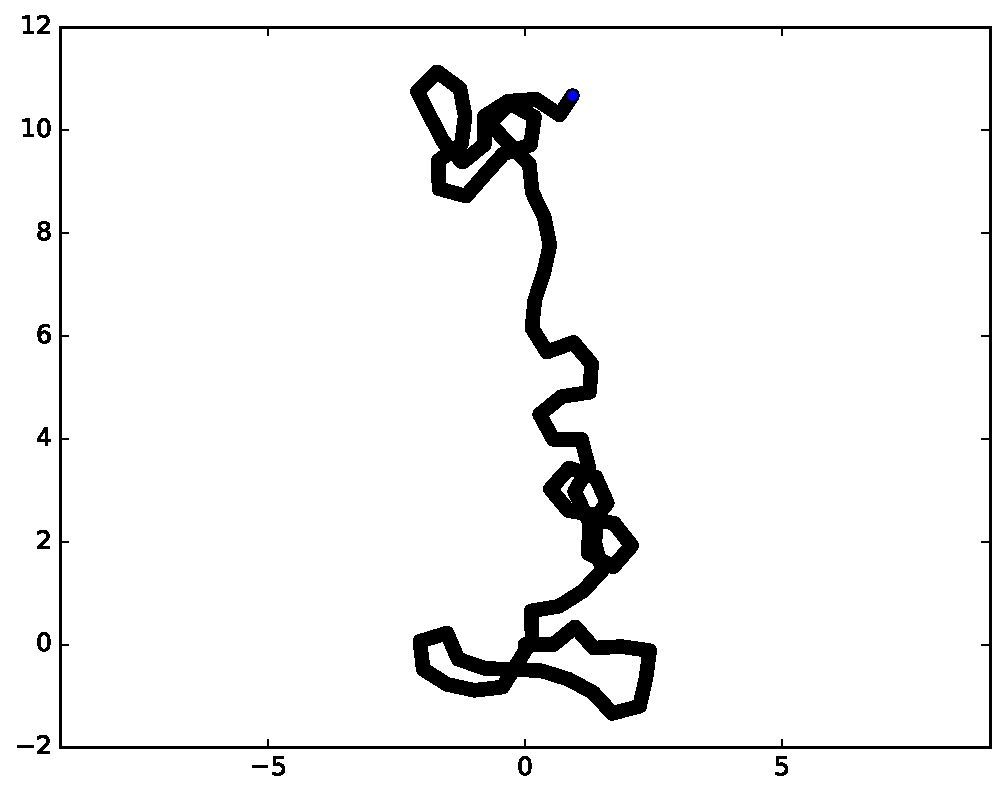
\includegraphics[width=\textwidth]{figures/ch3/synTraj_219_90_4}
			\caption[$A = 90$, $F=4$]{$A = 90$, $F=4$}
			\label{fig:synTraj_219_90_4}
		\end{subfigure}
		~
		\begin{subfigure}[t]{\subImgWmo}
			\centering
			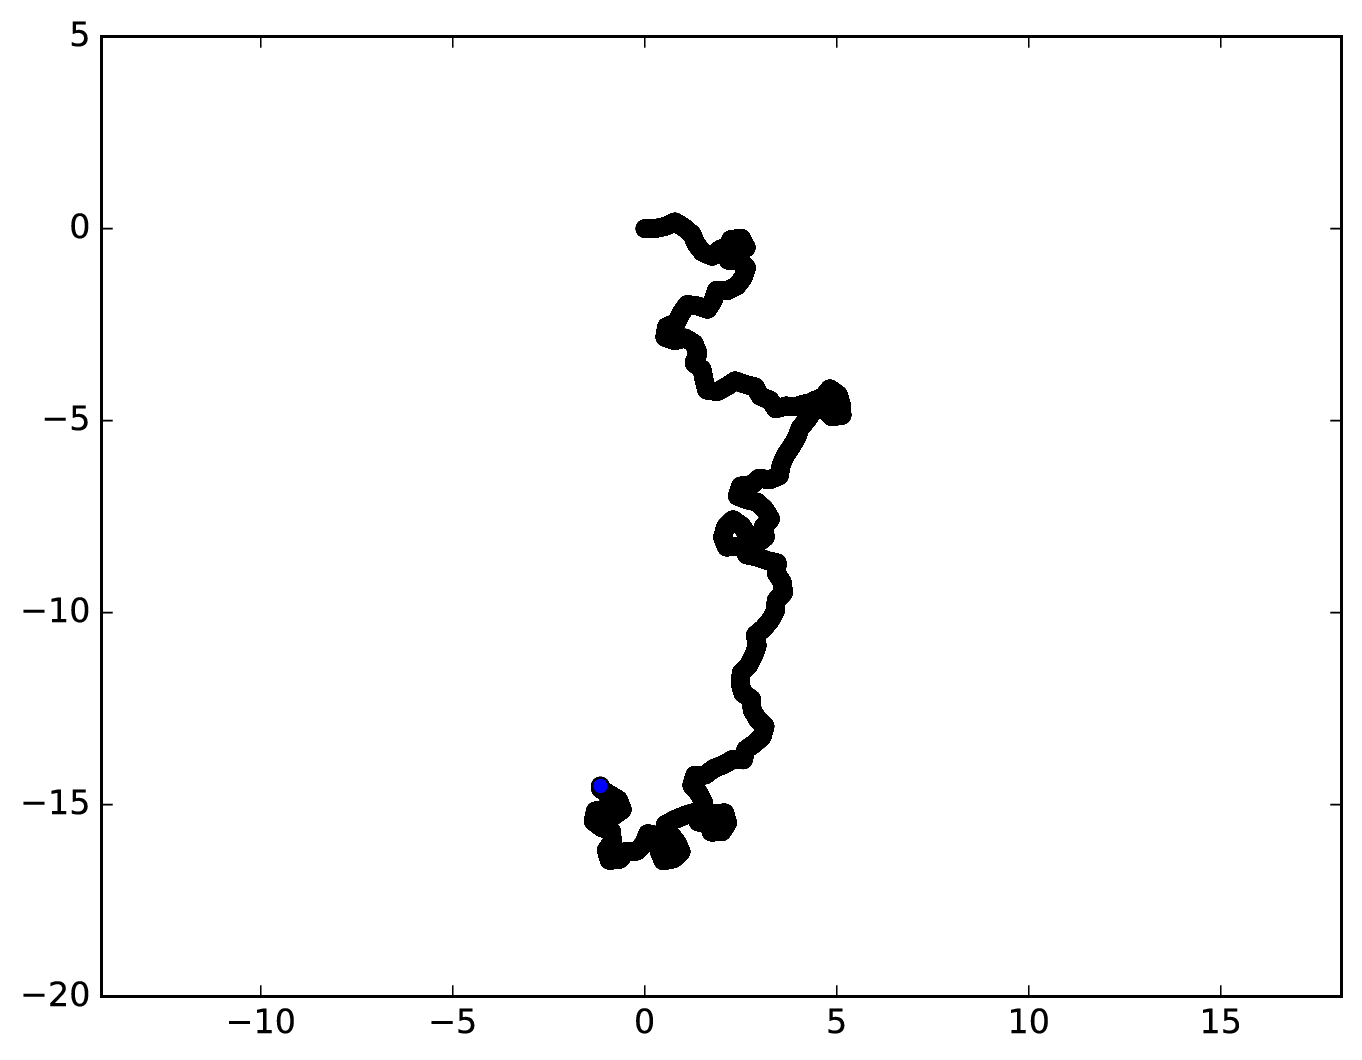
\includegraphics[width=\textwidth]{figures/ch3/synTraj_219_90_8}
			\caption[$A = 90$, $F=8$]{$A = 90$, $F=8$}
			\label{fig:synTraj_219_90_8}
		\end{subfigure}
		~
		\begin{subfigure}[t]{\subImgWmo}
			\centering
			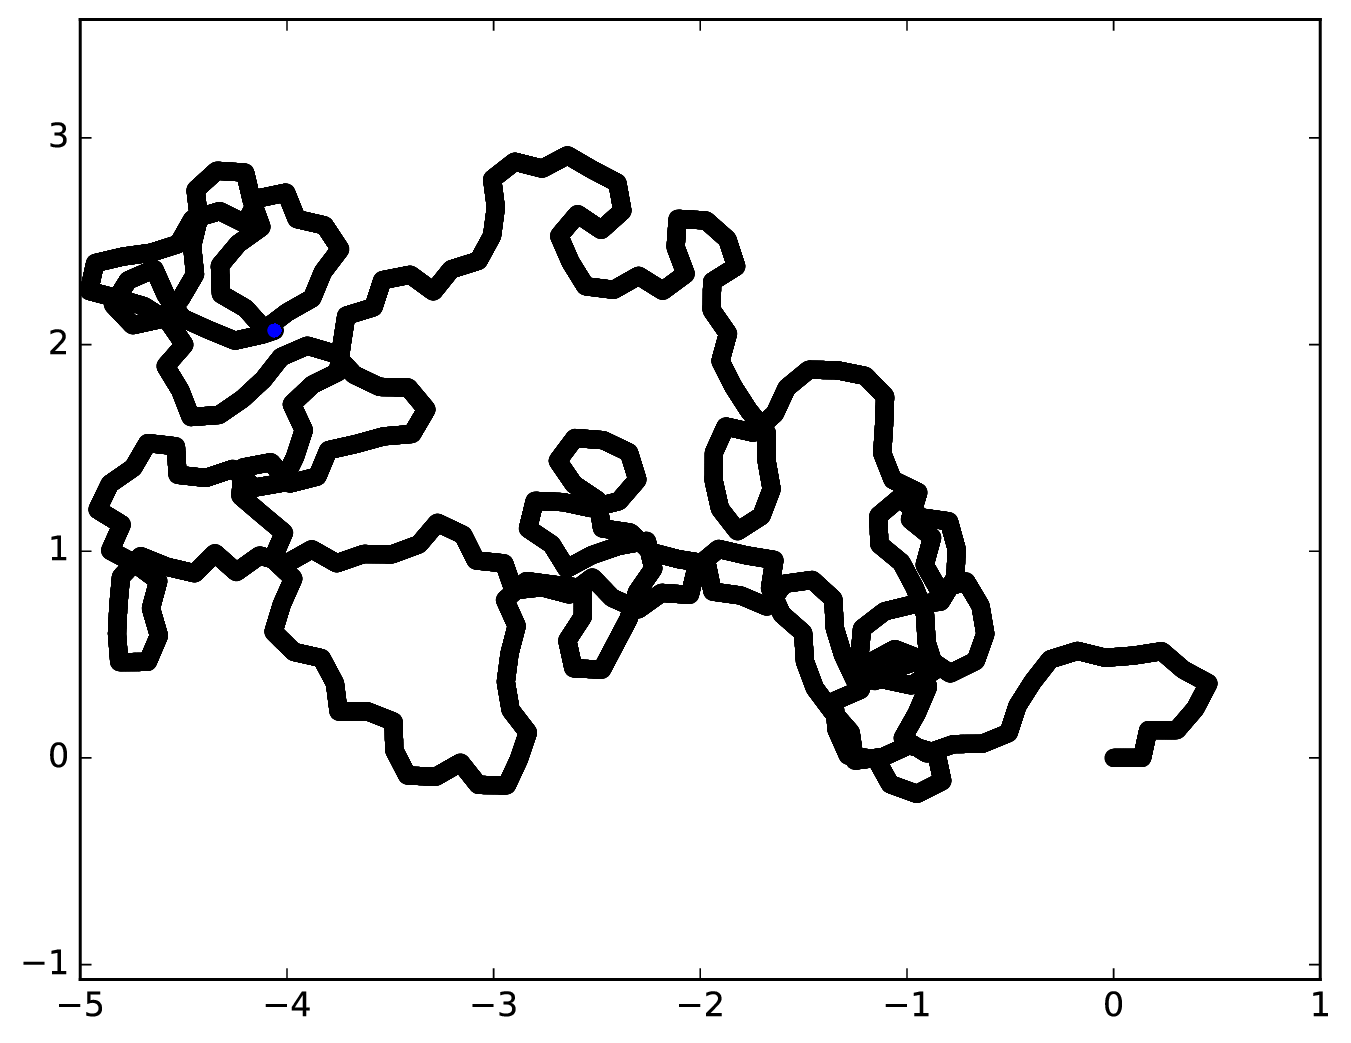
\includegraphics[width=\textwidth]{figures/ch3/synTraj_219_90_16}
			\caption[$A = 90$, $F=16$]{$A = 90$, $F=16$}
			\label{fig:synTraj_219_90_16}
		\end{subfigure}
		~
		\begin{subfigure}[t]{\subImgWmo}
			\centering
			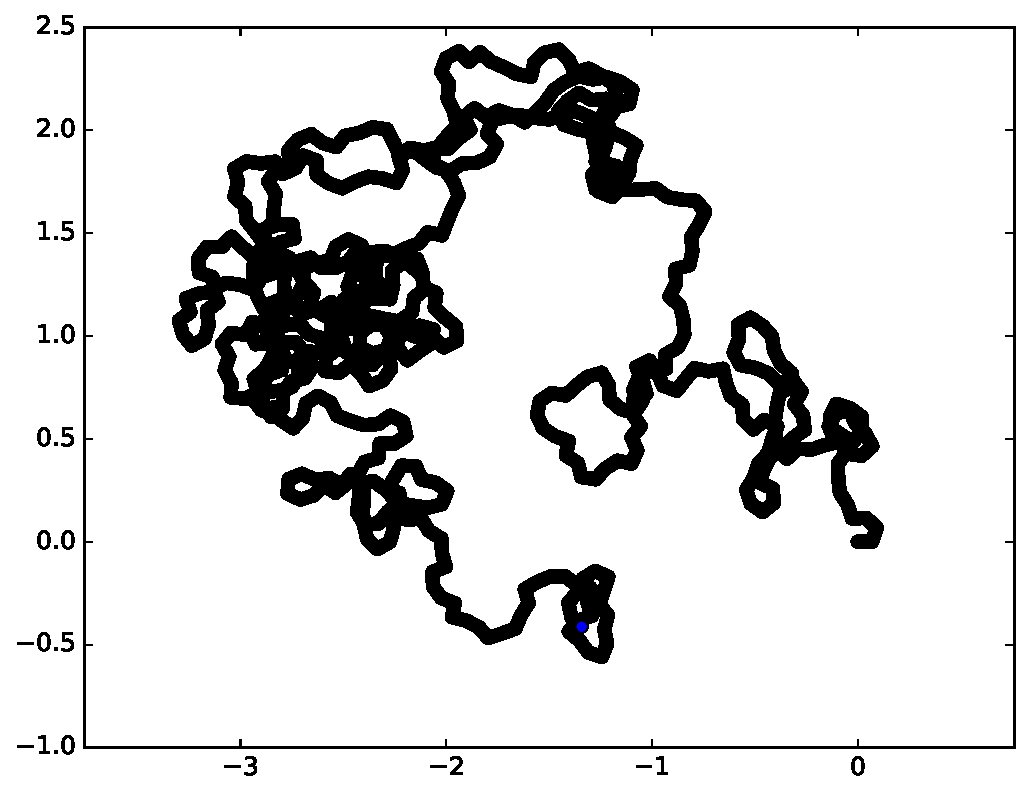
\includegraphics[width=\textwidth]{figures/ch3/synTraj_219_90_32}
			\caption[$A = 90$, $F=32$]{$A = 90$, $F=32$}
			\label{fig:synTraj_219_90_32}
		\end{subfigure}
		~
		\begin{subfigure}[t]{\subImgWmo}
			\centering
			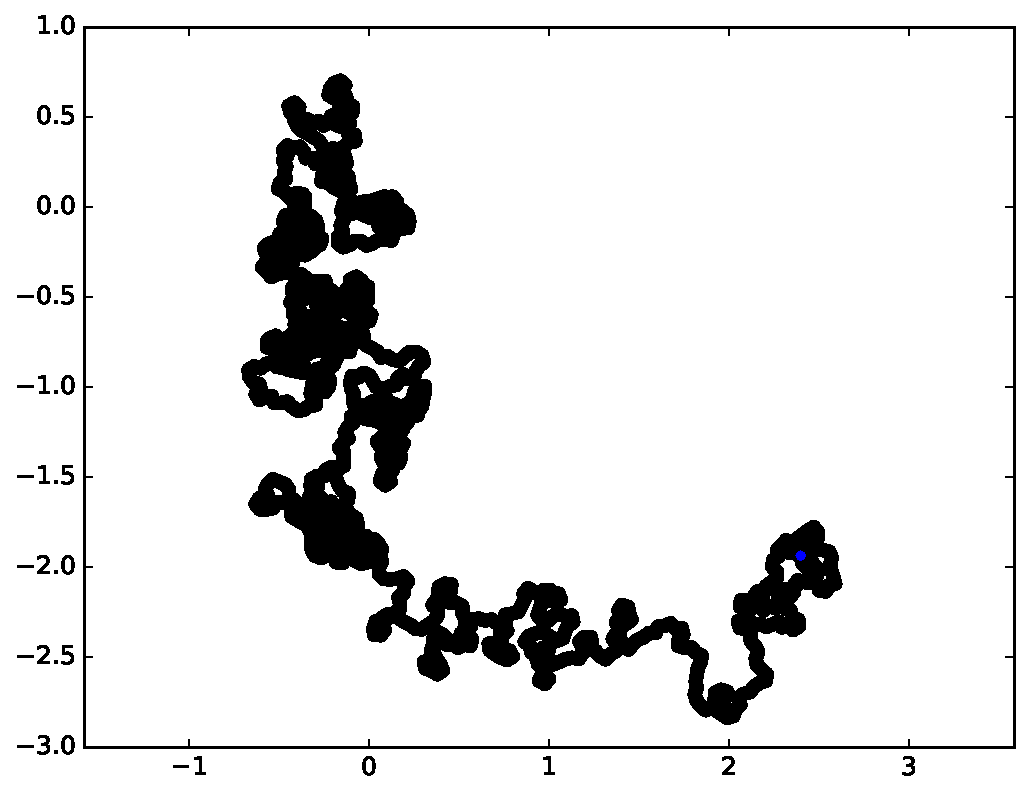
\includegraphics[width=\textwidth]{figures/ch3/synTraj_219_90_60}
			\caption[$A = 90$, $F=60$]{$A = 90$, $F=60$}
			\label{fig:synTraj_219_90_60}
		\end{subfigure}
		\caption[Mouvements générés par notre modèle -- III]{Exemples de trajectoires générées par notre modèle pour un objet de vitesse constante (2,19~cm/s).}
		\label{fig:motion7590}
	\end{figure}
	
	
	
	\begin{figure}[htb]
		\begin{subfigure}[t]{\subImgWmo}
			\centering
			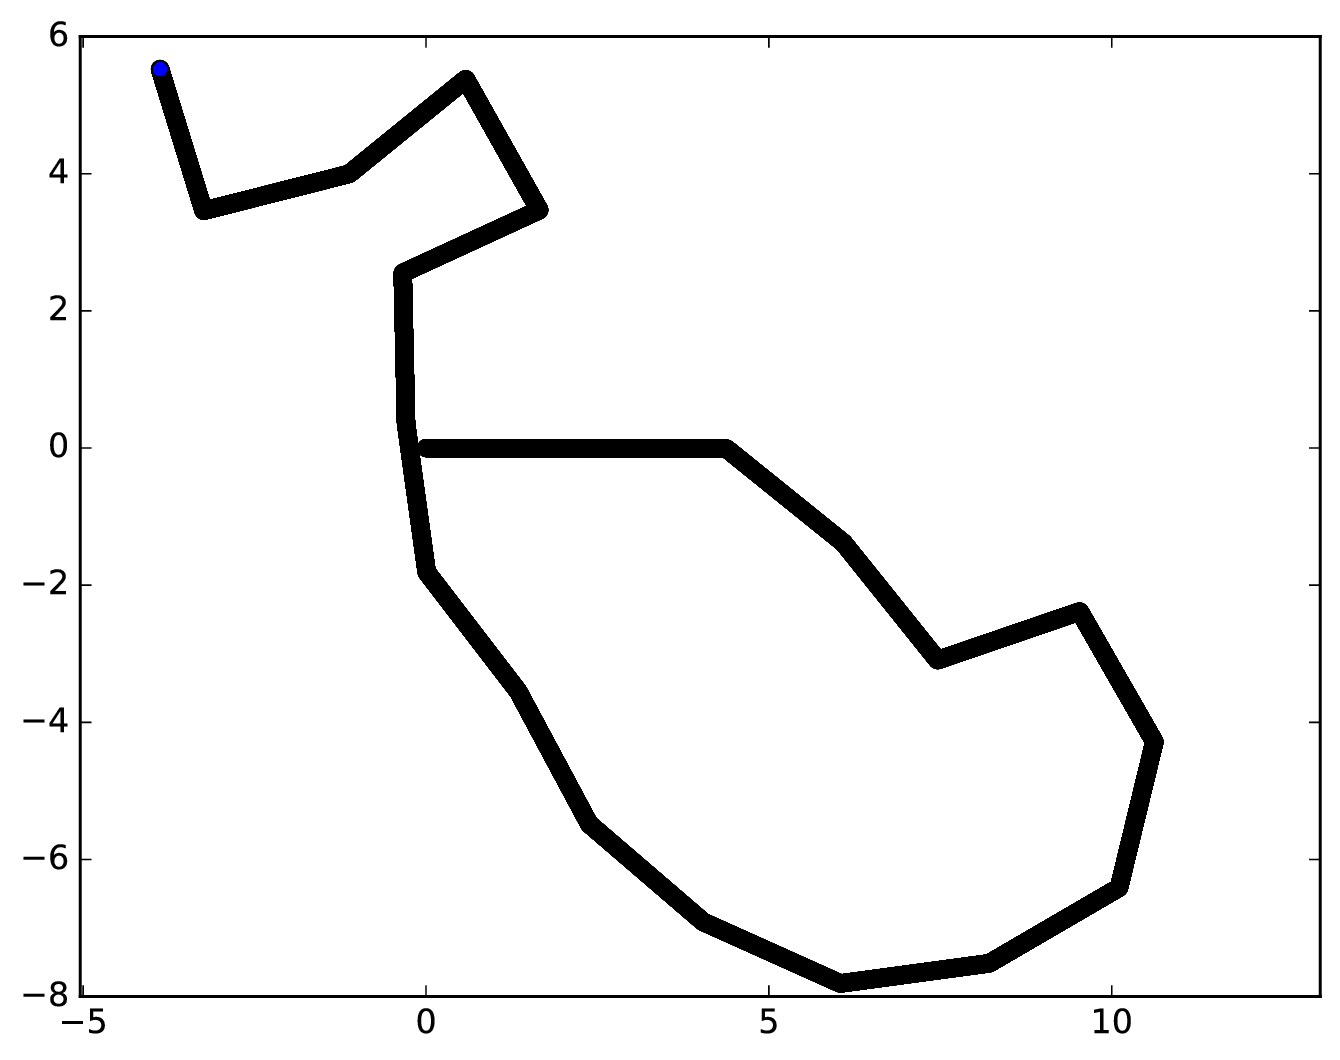
\includegraphics[width=\textwidth]{figures/ch3/synTraj_219_105_1}
			\caption[$A = 105$, $F=1$]{$A = 105$, $F=1$}
			\label{fig:synTraj_219_105_1}
		\end{subfigure}
		~
		\begin{subfigure}[t]{\subImgWmo}
			\centering
			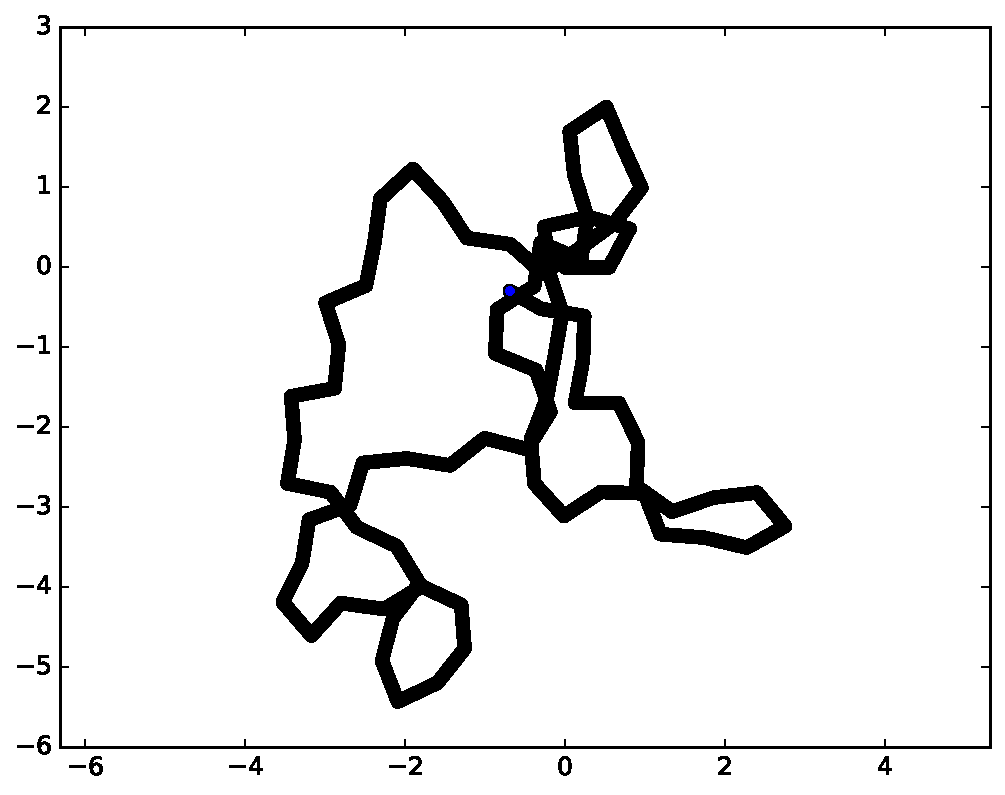
\includegraphics[width=\textwidth]{figures/ch3/synTraj_219_105_4}
			\caption[$A = 105$, $F=4$]{$A = 105$, $F=4$}
			\label{fig:synTraj_219_105_4}
		\end{subfigure}
		~
		\begin{subfigure}[t]{\subImgWmo}
			\centering
			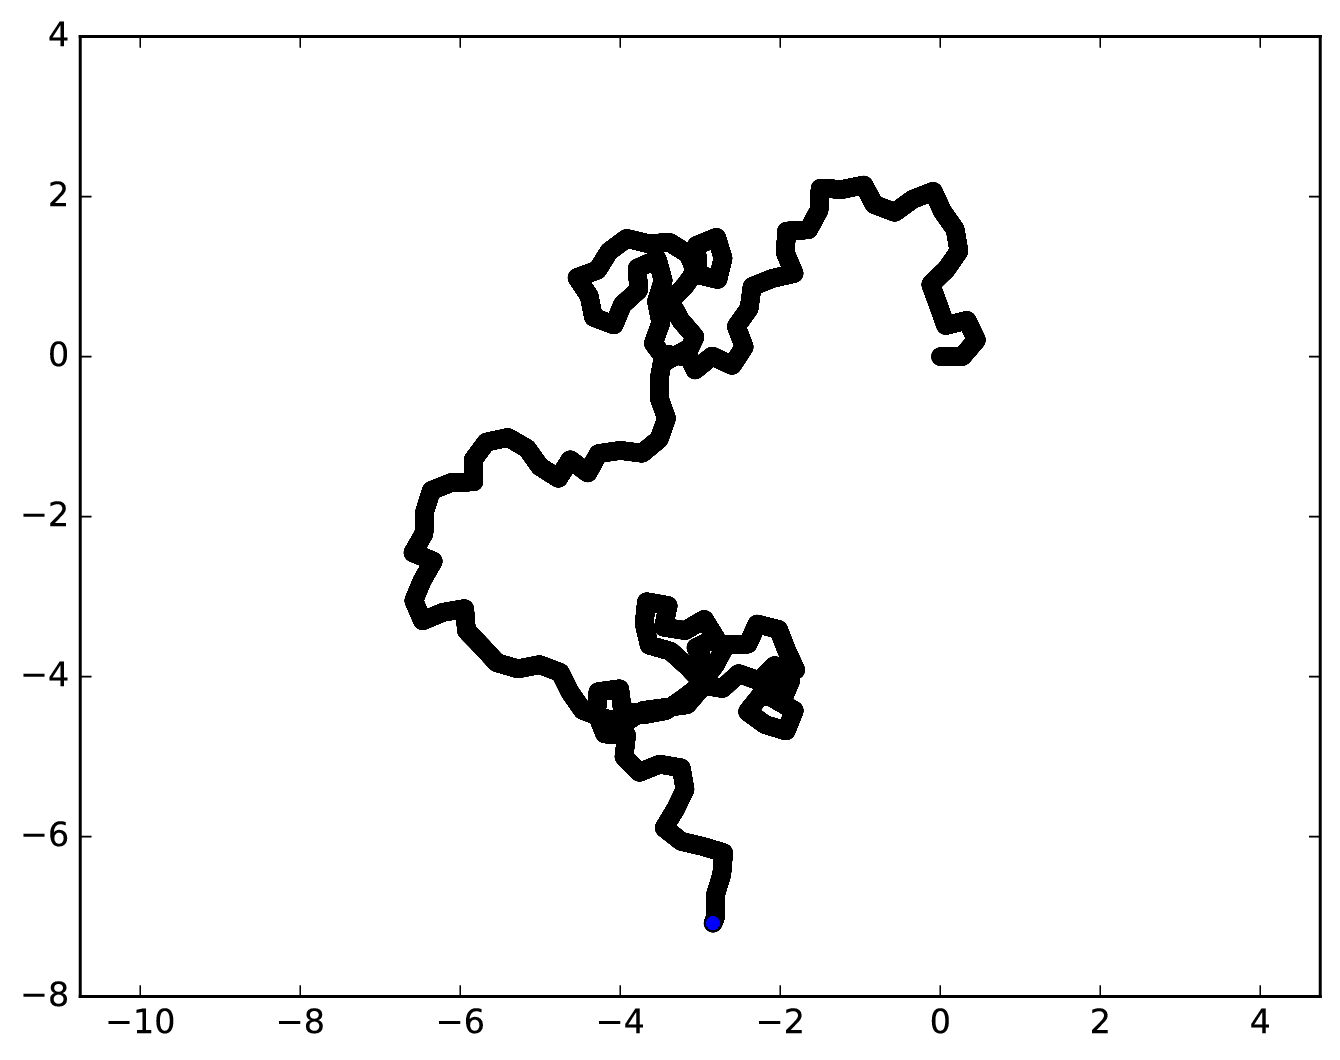
\includegraphics[width=\textwidth]{figures/ch3/synTraj_219_105_8}
			\caption[$A = 105$, $F=8$]{$A = 105$, $F=8$}
			\label{fig:synTraj_219_105_8}
		\end{subfigure}
		~
		\begin{subfigure}[t]{\subImgWmo}
			\centering
			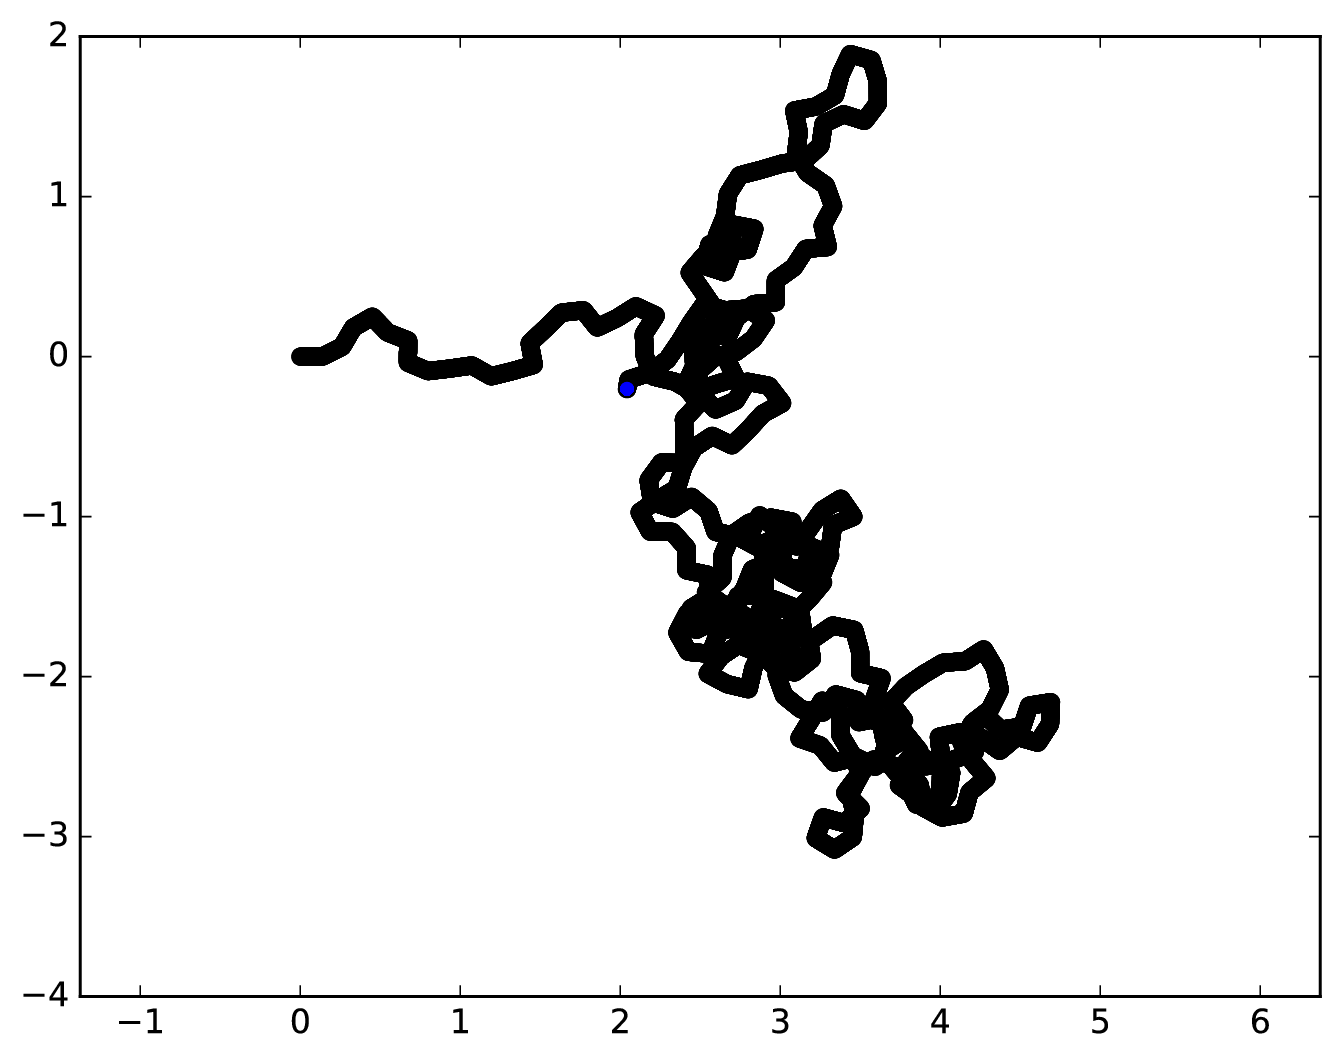
\includegraphics[width=\textwidth]{figures/ch3/synTraj_219_105_16}
			\caption[$A = 105$, $F=16$]{$A = 105$, $F=16$}
			\label{fig:synTraj_219_105_16}
		\end{subfigure}
		~
		\begin{subfigure}[t]{\subImgWmo}
			\centering
			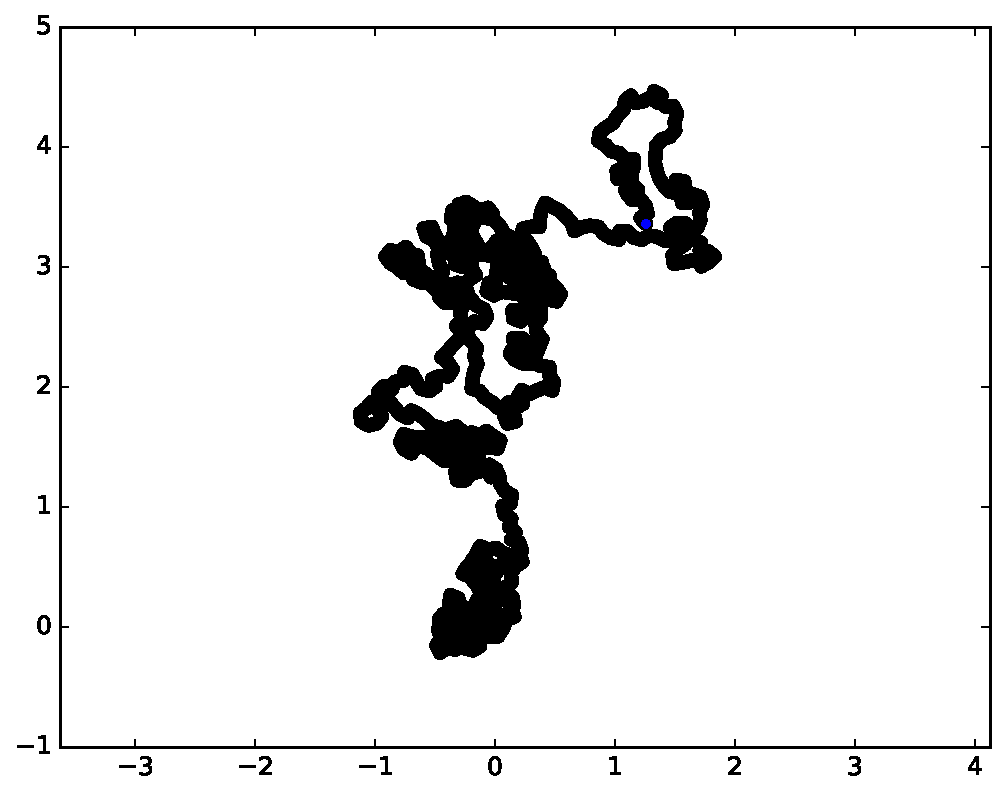
\includegraphics[width=\textwidth]{figures/ch3/synTraj_219_105_32}
			\caption[$A = 105$, $F=32$]{$A = 105$, $F=32$}
			\label{fig:synTraj_219_105_32}
		\end{subfigure}
		~
		\begin{subfigure}[t]{\subImgWmo}
			\centering
			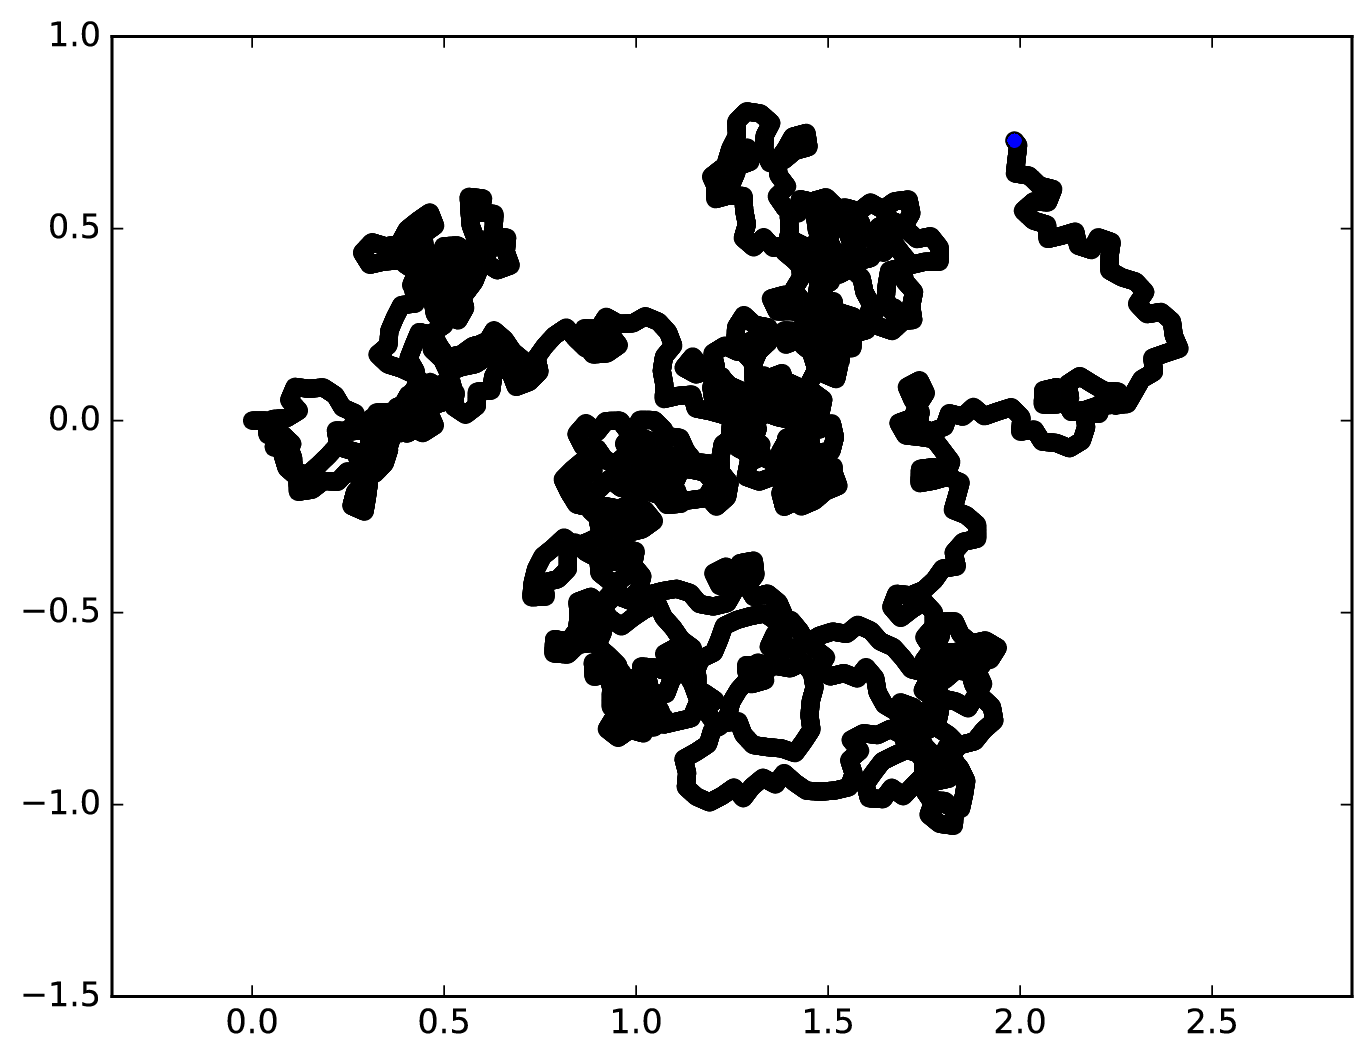
\includegraphics[width=\textwidth]{figures/ch3/synTraj_219_105_60}
			\caption[$A = 105$, $F=60$]{$A = 105$, $F=60$}
			\label{fig:synTraj_219_105_60}
		\end{subfigure}
		~
		\begin{subfigure}[t]{\subImgWmo}
			\centering
			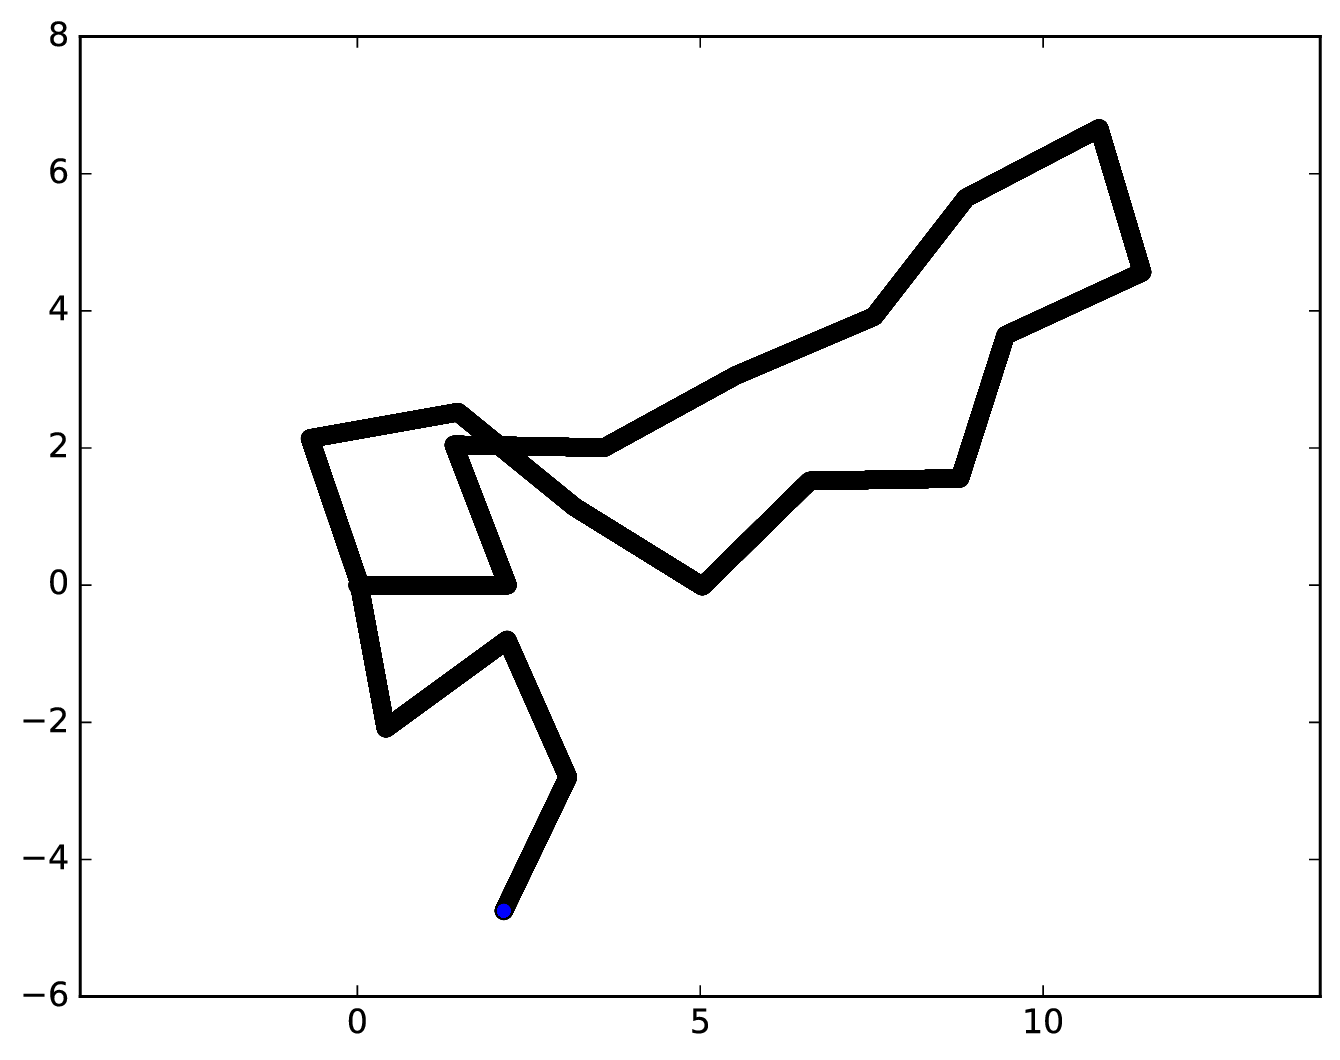
\includegraphics[width=\textwidth]{figures/ch3/synTraj_219_120_1}
			\caption[$A = 120$, $F=1$]{$A = 120$, $F=1$}
			\label{fig:synTraj_219_120_1}
		\end{subfigure}
		~
		\begin{subfigure}[t]{\subImgWmo}
			\centering
			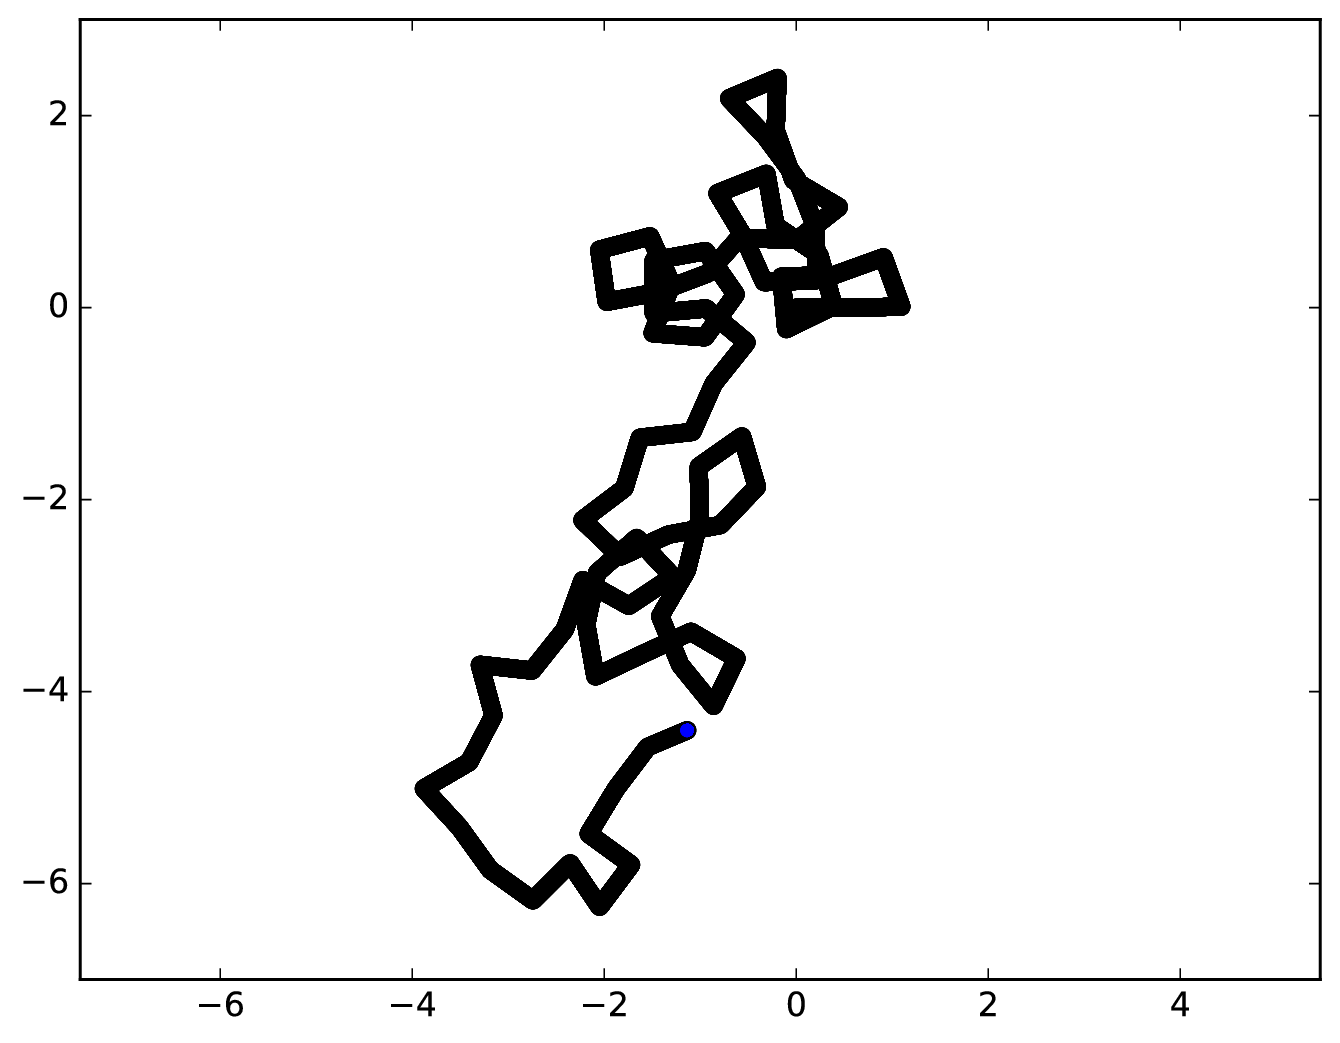
\includegraphics[width=\textwidth]{figures/ch3/synTraj_219_120_4}
			\caption[$A = 120$, $F=4$]{$A = 120$, $F=4$}
			\label{fig:synTraj_219_120_4}
		\end{subfigure}
		~
		\begin{subfigure}[t]{\subImgWmo}
			\centering
			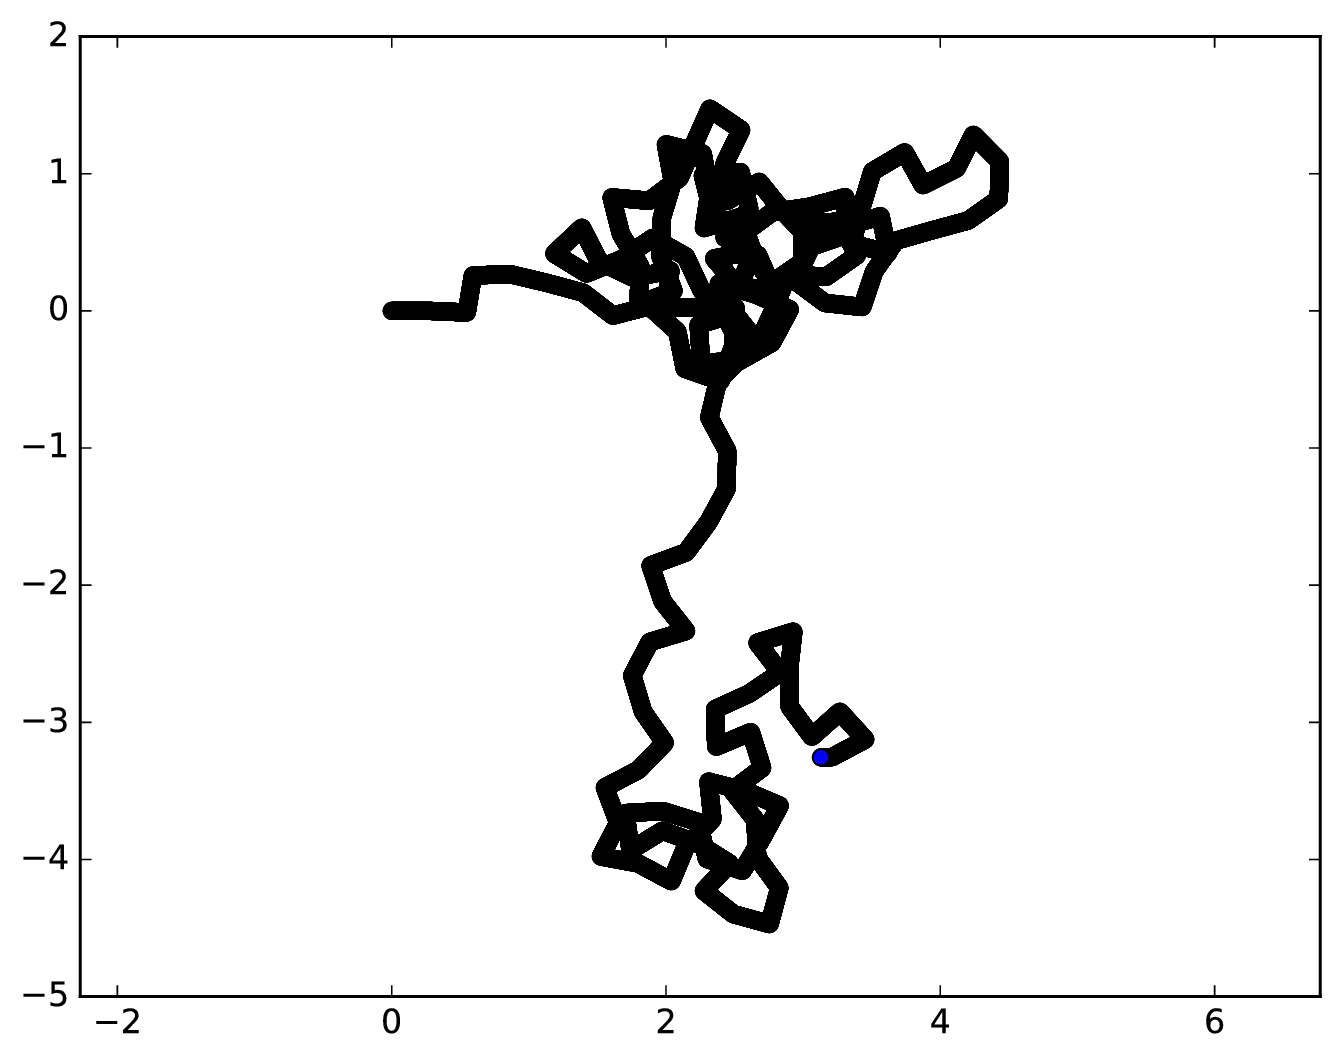
\includegraphics[width=\textwidth]{figures/ch3/synTraj_219_120_8}
			\caption[$A = 120$, $F=8$]{$A = 120$, $F=8$}
			\label{fig:synTraj_219_120_8}
		\end{subfigure}
		~
		\begin{subfigure}[t]{\subImgWmo}
			\centering
			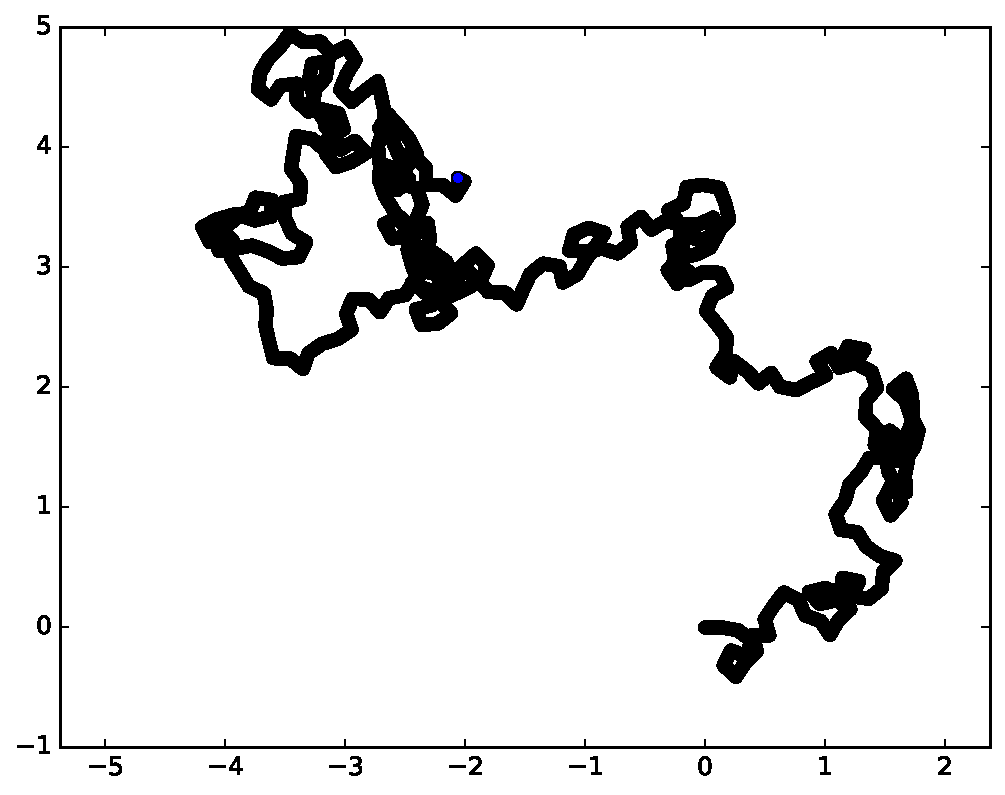
\includegraphics[width=\textwidth]{figures/ch3/synTraj_219_120_16}
			\caption[$A = 120$, $F=16$]{$A = 120$, $F=16$}
			\label{fig:synTraj_219_120_16}
		\end{subfigure}
		~
		\begin{subfigure}[t]{\subImgWmo}
			\centering
			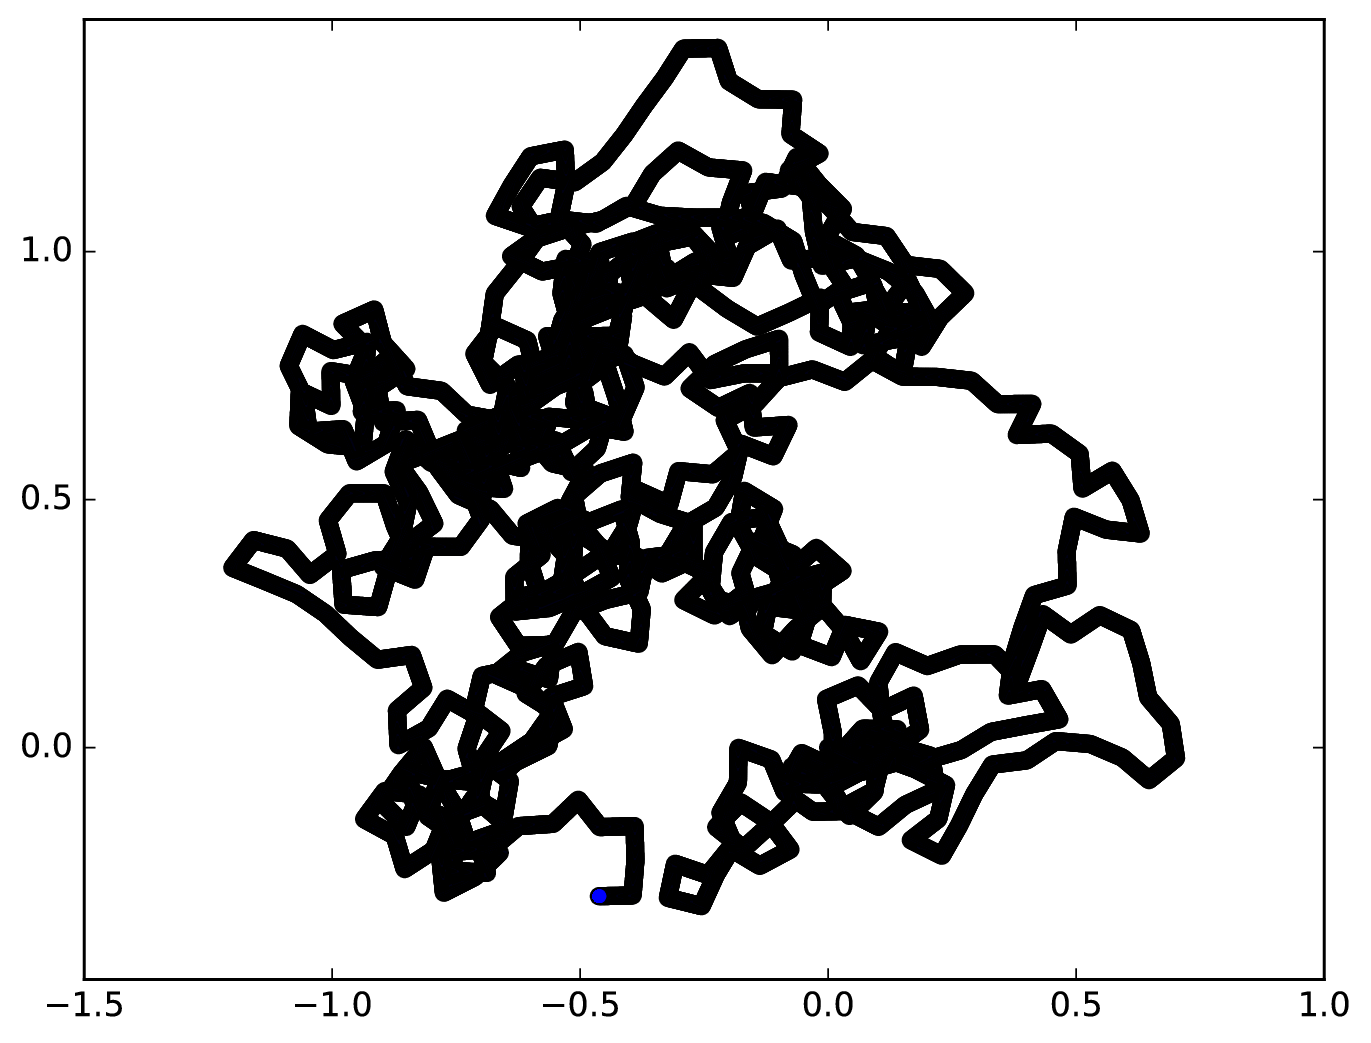
\includegraphics[width=\textwidth]{figures/ch3/synTraj_219_120_32}
			\caption[$A = 120$, $F=32$]{$A = 120$, $F=32$}
			\label{fig:synTraj_219_120_32}
		\end{subfigure}
		~
		\begin{subfigure}[t]{\subImgWmo}
			\centering
			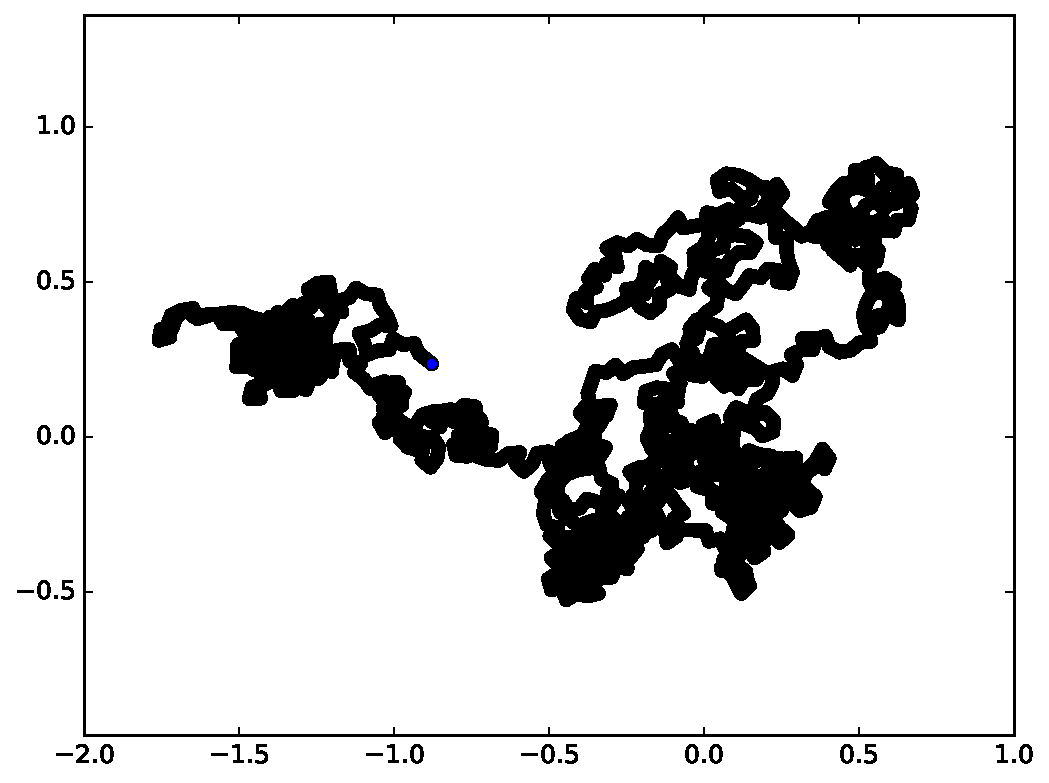
\includegraphics[width=\textwidth]{figures/ch3/synTraj_219_120_60}
			\caption[$A = 120$, $F=60$]{$A = 120$, $F=60$}
			\label{fig:synTraj_219_120_60}
		\end{subfigure}
		\caption[Mouvements générés par notre modèle -- IV]{Exemples de trajectoires générées par notre modèle pour un objet de vitesse constante (2,19~cm/s).}
		\label{fig:motion105120}
	\end{figure}
	
	
	
	\begin{figure}[htb]
		\begin{subfigure}[t]{\subImgWmo}
			\centering
			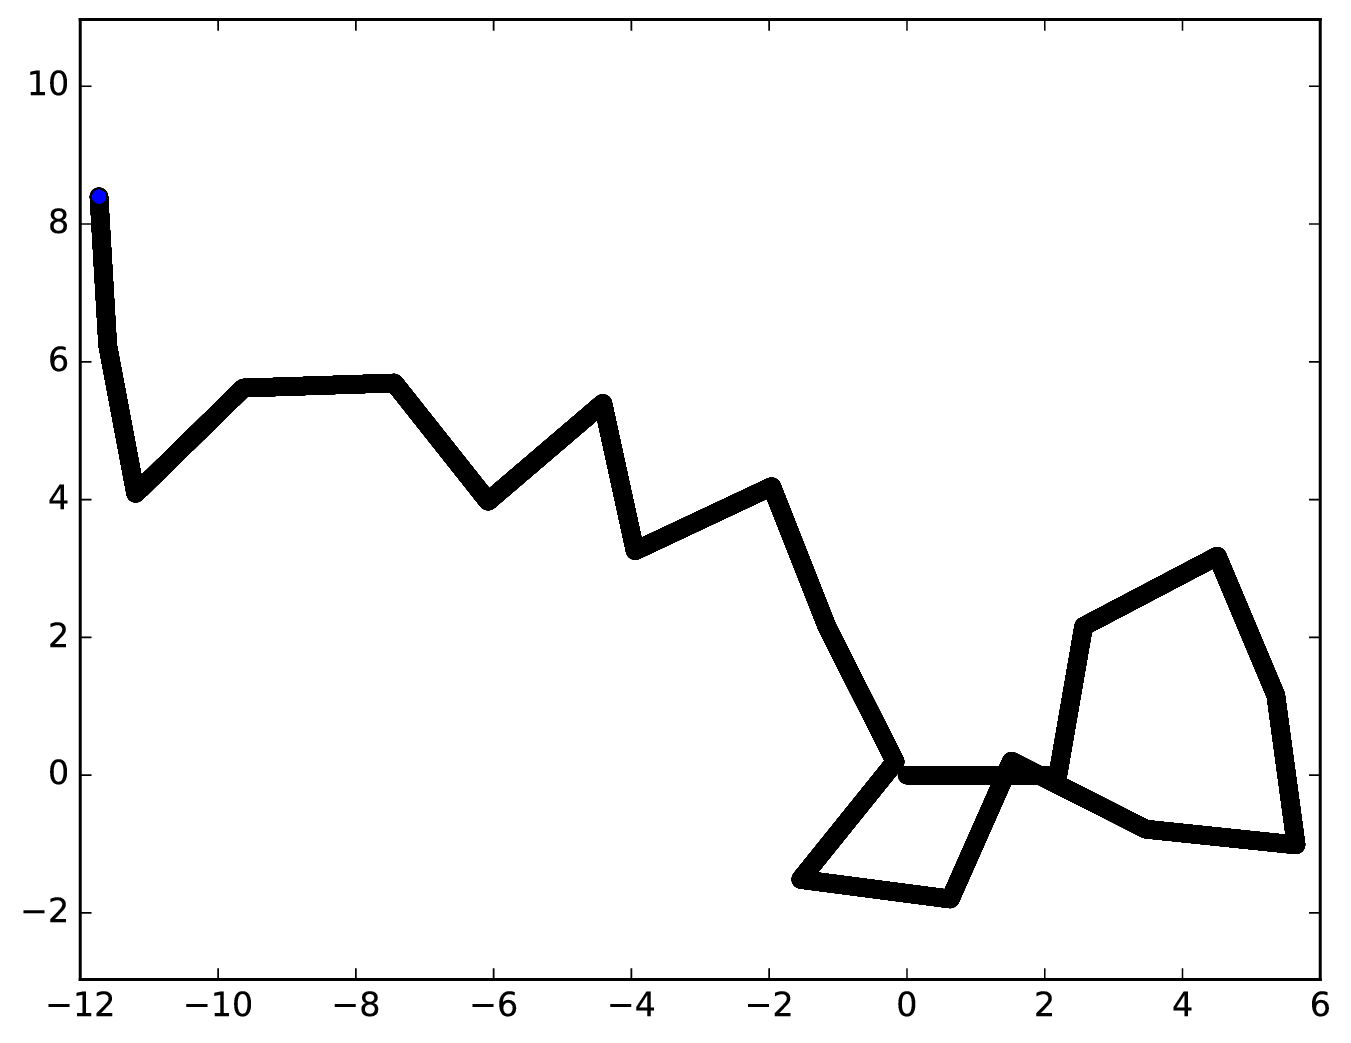
\includegraphics[width=\textwidth]{figures/ch3/synTraj_219_135_1}
			\caption[$A = 135$, $F=1$]{$A = 135$, $F=1$}
			\label{fig:synTraj_219_135_1}
		\end{subfigure}
		~
		\begin{subfigure}[t]{\subImgWmo}
			\centering
			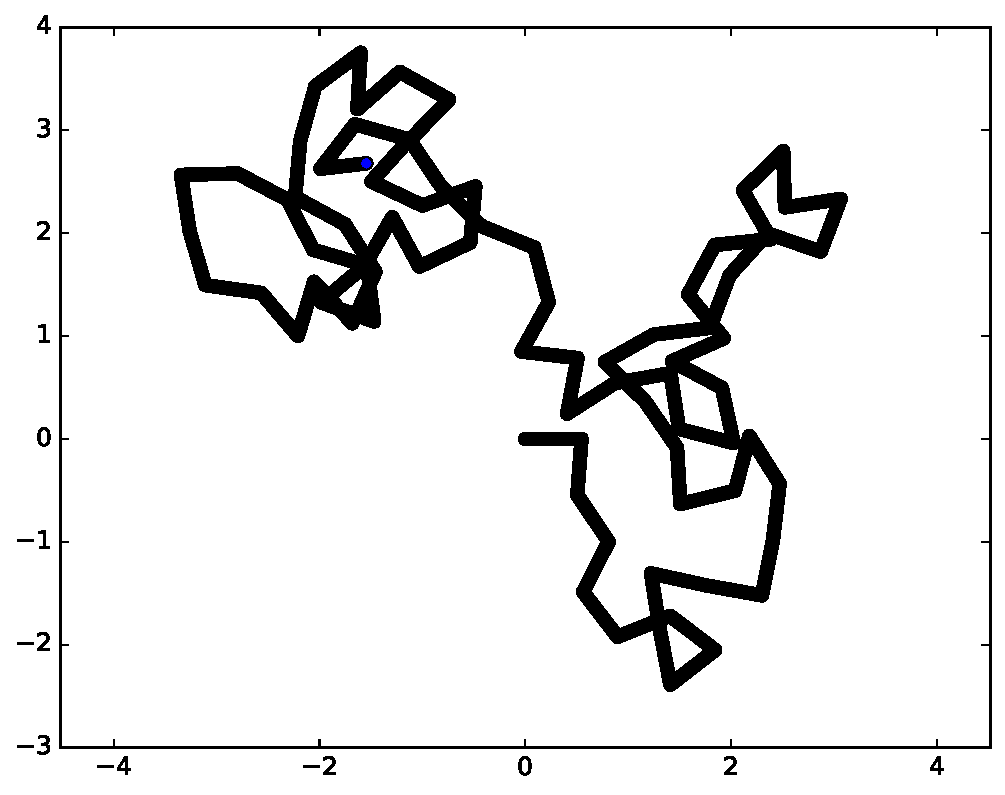
\includegraphics[width=\textwidth]{figures/ch3/synTraj_219_135_4}
			\caption[$A = 135$, $F=4$]{$A = 135$, $F=4$}
			\label{fig:synTraj_219_135_4}
		\end{subfigure}
		~
		\begin{subfigure}[t]{\subImgWmo}
			\centering
			\includegraphics[width=\textwidth]{figures/ch3/synTraj_219_135_8}
			\caption[$A = 135$, $F=8$]{$A = 135$, $F=8$}
			\label{fig:synTraj_219_135_8}
		\end{subfigure}
		~
		\begin{subfigure}[t]{\subImgWmo}
			\centering
			\includegraphics[width=\textwidth]{figures/ch3/synTraj_219_135_16}
			\caption[$A = 135$, $F=16$]{$A = 135$, $F=16$}
			\label{fig:synTraj_219_135_16}
		\end{subfigure}
		~
		\begin{subfigure}[t]{\subImgWmo}
			\centering
			\includegraphics[width=\textwidth]{figures/ch3/synTraj_219_135_32}
			\caption[$A = 135$, $F=32$]{$A = 135$, $F=32$}
			\label{fig:synTraj_219_135_32}
		\end{subfigure}
		~
		\begin{subfigure}[t]{\subImgWmo}
			\centering
			\includegraphics[width=\textwidth]{figures/ch3/synTraj_219_135_60}
			\caption[$A = 135$, $F=60$]{$A = 135$, $F=60$}
			\label{fig:synTraj_219_135_60}
		\end{subfigure}
		~
		\begin{subfigure}[t]{\subImgWmo}
			\centering
			\includegraphics[width=\textwidth]{figures/ch3/synTraj_219_150_1}
			\caption[$A = 150$, $F=1$]{$A = 150$, $F=1$}
			\label{fig:synTraj_219_150_1}
		\end{subfigure}
		~
		\begin{subfigure}[t]{\subImgWmo}
			\centering
			\includegraphics[width=\textwidth]{figures/ch3/synTraj_219_150_4}
			\caption[$A = 150$, $F=4$]{$A = 150$, $F=4$}
			\label{fig:synTraj_219_150_4}
		\end{subfigure}
		~
		\begin{subfigure}[t]{\subImgWmo}
			\centering
			\includegraphics[width=\textwidth]{figures/ch3/synTraj_219_150_8}
			\caption[$A = 150$, $F=8$]{$A = 150$, $F=8$}
			\label{fig:synTraj_219_150_8}
		\end{subfigure}
		~
		\begin{subfigure}[t]{\subImgWmo}
			\centering
			\includegraphics[width=\textwidth]{figures/ch3/synTraj_219_150_16}
			\caption[$A = 150$, $F=16$]{$A = 150$, $F=16$}
			\label{fig:synTraj_219_150_16}
		\end{subfigure}
		~
		\begin{subfigure}[t]{\subImgWmo}
			\centering
			\includegraphics[width=\textwidth]{figures/ch3/synTraj_219_150_32}
			\caption[$A = 150$, $F=32$]{$A = 150$, $F=32$}
			\label{fig:synTraj_219_150_32}
		\end{subfigure}
		~
		\begin{subfigure}[t]{\subImgWmo}
			\centering
			\includegraphics[width=\textwidth]{figures/ch3/synTraj_219_150_60}
			\caption[$A = 150$, $F=60$]{$A = 150$, $F=60$}
			\label{fig:synTraj_219_150_60}
		\end{subfigure}
		\caption[Mouvements générés par notre modèle -- V]{Exemples de trajectoires générées par notre modèle pour un objet de vitesse constante (2,19~cm/s).}
		\label{fig:motion135150}
	\end{figure}
	
	
	
	\begin{figure}[htb]
		\begin{subfigure}[t]{\subImgWmo}
			\centering
			\includegraphics[width=\textwidth]{figures/ch3/synTraj_219_165_1}
			\caption[$A = 165$, $F=1$]{$A = 165$, $F=1$}
			\label{fig:synTraj_219_165_1}
		\end{subfigure}
		~
		\begin{subfigure}[t]{\subImgWmo}
			\centering
			\includegraphics[width=\textwidth]{figures/ch3/synTraj_219_165_4}
			\caption[$A = 165$, $F=4$]{$A = 165$, $F=4$}
			\label{fig:synTraj_219_165_4}
		\end{subfigure}
		~
		\begin{subfigure}[t]{\subImgWmo}
			\centering
			\includegraphics[width=\textwidth]{figures/ch3/synTraj_219_165_8}
			\caption[$A = 165$, $F=8$]{$A = 165$, $F=8$}
			\label{fig:synTraj_219_165_8}
		\end{subfigure}
		~
		\begin{subfigure}[t]{\subImgWmo}
			\centering
			\includegraphics[width=\textwidth]{figures/ch3/synTraj_219_165_16}
			\caption[$A = 165$, $F=16$]{$A = 165$, $F=16$}
			\label{fig:synTraj_219_165_16}
		\end{subfigure}
		~
		\begin{subfigure}[t]{\subImgWmo}
			\centering
			\includegraphics[width=\textwidth]{figures/ch3/synTraj_219_165_32}
			\caption[$A = 165$, $F=32$]{$A = 165$, $F=32$}
			\label{fig:synTraj_219_165_32}
		\end{subfigure}
		~
		\begin{subfigure}[t]{\subImgWmo}
			\centering
			\includegraphics[width=\textwidth]{figures/ch3/synTraj_219_165_60}
			\caption[$A = 165$, $F=60$]{$A = 165$, $F=60$}
			\label{fig:synTraj_219_165_60}
		\end{subfigure}
		~
		\begin{subfigure}[t]{\subImgWmo}
			\centering
			\includegraphics[width=\textwidth]{figures/ch3/synTraj_219_180_1}
			\caption[$A = 180$, $F=1$]{$A = 180$, $F=1$}
			\label{fig:synTraj_219_180_1}
		\end{subfigure}
		~
		\begin{subfigure}[t]{\subImgWmo}
			\centering
			\includegraphics[width=\textwidth]{figures/ch3/synTraj_219_180_4}
			\caption[$A = 180$, $F=4$]{$A = 180$, $F=4$}
			\label{fig:synTraj_219_180_4}
		\end{subfigure}
		~
		\begin{subfigure}[t]{\subImgWmo}
			\centering
			\includegraphics[width=\textwidth]{figures/ch3/synTraj_219_180_8}
			\caption[$A = 180$, $F=1$]{$A = 180$, $F=8$}
			\label{fig:synTraj_219_180_8}
		\end{subfigure}
		~
		\begin{subfigure}[t]{\subImgWmo}
			\centering
			\includegraphics[width=\textwidth]{figures/ch3/synTraj_219_180_16}
			\caption[$A = 180$, $F=16$]{$A = 1805$, $F=16$}
			\label{fig:synTraj_219_180_16}
		\end{subfigure}
		~
		\begin{subfigure}[t]{\subImgWmo}
			\centering
			\includegraphics[width=\textwidth]{figures/ch3/synTraj_219_180_32}
			\caption[$A = 180$, $F=32$]{$A = 180$, $F=32$}
			\label{fig:synTraj_219_180_32}
		\end{subfigure}
		~
		\begin{subfigure}[t]{\subImgWmo}
			\centering
			\includegraphics[width=\textwidth]{figures/ch3/synTraj_219_180_60}
			\caption[$A = 180$, $F=60$]{$A = 180$, $F=60$}
			\label{fig:synTraj_219_180_60}
		\end{subfigure}
		\caption[Mouvements générés par notre modèle -- VI]{Exemples de trajectoires générées par notre modèle pour un objet de vitesse constante (2,19~cm/s).}
		\label{fig:motion165180}
	\end{figure}
	
	
    \subsection{Résultats}
    Dynamique moléculaire. Foules ? Jeux vidéo ? Autres ?


\section{Conclusion}

\clearpage
